% Options for packages loaded elsewhere
\PassOptionsToPackage{unicode}{hyperref}
\PassOptionsToPackage{hyphens}{url}
%
\documentclass[
]{book}
\usepackage{amsmath,amssymb}
\usepackage{iftex}
\ifPDFTeX
  \usepackage[T1]{fontenc}
  \usepackage[utf8]{inputenc}
  \usepackage{textcomp} % provide euro and other symbols
\else % if luatex or xetex
  \usepackage{unicode-math} % this also loads fontspec
  \defaultfontfeatures{Scale=MatchLowercase}
  \defaultfontfeatures[\rmfamily]{Ligatures=TeX,Scale=1}
\fi
\usepackage{lmodern}
\ifPDFTeX\else
  % xetex/luatex font selection
\fi
% Use upquote if available, for straight quotes in verbatim environments
\IfFileExists{upquote.sty}{\usepackage{upquote}}{}
\IfFileExists{microtype.sty}{% use microtype if available
  \usepackage[]{microtype}
  \UseMicrotypeSet[protrusion]{basicmath} % disable protrusion for tt fonts
}{}
\makeatletter
\@ifundefined{KOMAClassName}{% if non-KOMA class
  \IfFileExists{parskip.sty}{%
    \usepackage{parskip}
  }{% else
    \setlength{\parindent}{0pt}
    \setlength{\parskip}{6pt plus 2pt minus 1pt}}
}{% if KOMA class
  \KOMAoptions{parskip=half}}
\makeatother
\usepackage{xcolor}
\usepackage{color}
\usepackage{fancyvrb}
\newcommand{\VerbBar}{|}
\newcommand{\VERB}{\Verb[commandchars=\\\{\}]}
\DefineVerbatimEnvironment{Highlighting}{Verbatim}{commandchars=\\\{\}}
% Add ',fontsize=\small' for more characters per line
\usepackage{framed}
\definecolor{shadecolor}{RGB}{248,248,248}
\newenvironment{Shaded}{\begin{snugshade}}{\end{snugshade}}
\newcommand{\AlertTok}[1]{\textcolor[rgb]{0.94,0.16,0.16}{#1}}
\newcommand{\AnnotationTok}[1]{\textcolor[rgb]{0.56,0.35,0.01}{\textbf{\textit{#1}}}}
\newcommand{\AttributeTok}[1]{\textcolor[rgb]{0.13,0.29,0.53}{#1}}
\newcommand{\BaseNTok}[1]{\textcolor[rgb]{0.00,0.00,0.81}{#1}}
\newcommand{\BuiltInTok}[1]{#1}
\newcommand{\CharTok}[1]{\textcolor[rgb]{0.31,0.60,0.02}{#1}}
\newcommand{\CommentTok}[1]{\textcolor[rgb]{0.56,0.35,0.01}{\textit{#1}}}
\newcommand{\CommentVarTok}[1]{\textcolor[rgb]{0.56,0.35,0.01}{\textbf{\textit{#1}}}}
\newcommand{\ConstantTok}[1]{\textcolor[rgb]{0.56,0.35,0.01}{#1}}
\newcommand{\ControlFlowTok}[1]{\textcolor[rgb]{0.13,0.29,0.53}{\textbf{#1}}}
\newcommand{\DataTypeTok}[1]{\textcolor[rgb]{0.13,0.29,0.53}{#1}}
\newcommand{\DecValTok}[1]{\textcolor[rgb]{0.00,0.00,0.81}{#1}}
\newcommand{\DocumentationTok}[1]{\textcolor[rgb]{0.56,0.35,0.01}{\textbf{\textit{#1}}}}
\newcommand{\ErrorTok}[1]{\textcolor[rgb]{0.64,0.00,0.00}{\textbf{#1}}}
\newcommand{\ExtensionTok}[1]{#1}
\newcommand{\FloatTok}[1]{\textcolor[rgb]{0.00,0.00,0.81}{#1}}
\newcommand{\FunctionTok}[1]{\textcolor[rgb]{0.13,0.29,0.53}{\textbf{#1}}}
\newcommand{\ImportTok}[1]{#1}
\newcommand{\InformationTok}[1]{\textcolor[rgb]{0.56,0.35,0.01}{\textbf{\textit{#1}}}}
\newcommand{\KeywordTok}[1]{\textcolor[rgb]{0.13,0.29,0.53}{\textbf{#1}}}
\newcommand{\NormalTok}[1]{#1}
\newcommand{\OperatorTok}[1]{\textcolor[rgb]{0.81,0.36,0.00}{\textbf{#1}}}
\newcommand{\OtherTok}[1]{\textcolor[rgb]{0.56,0.35,0.01}{#1}}
\newcommand{\PreprocessorTok}[1]{\textcolor[rgb]{0.56,0.35,0.01}{\textit{#1}}}
\newcommand{\RegionMarkerTok}[1]{#1}
\newcommand{\SpecialCharTok}[1]{\textcolor[rgb]{0.81,0.36,0.00}{\textbf{#1}}}
\newcommand{\SpecialStringTok}[1]{\textcolor[rgb]{0.31,0.60,0.02}{#1}}
\newcommand{\StringTok}[1]{\textcolor[rgb]{0.31,0.60,0.02}{#1}}
\newcommand{\VariableTok}[1]{\textcolor[rgb]{0.00,0.00,0.00}{#1}}
\newcommand{\VerbatimStringTok}[1]{\textcolor[rgb]{0.31,0.60,0.02}{#1}}
\newcommand{\WarningTok}[1]{\textcolor[rgb]{0.56,0.35,0.01}{\textbf{\textit{#1}}}}
\usepackage{longtable,booktabs,array}
\usepackage{calc} % for calculating minipage widths
% Correct order of tables after \paragraph or \subparagraph
\usepackage{etoolbox}
\makeatletter
\patchcmd\longtable{\par}{\if@noskipsec\mbox{}\fi\par}{}{}
\makeatother
% Allow footnotes in longtable head/foot
\IfFileExists{footnotehyper.sty}{\usepackage{footnotehyper}}{\usepackage{footnote}}
\makesavenoteenv{longtable}
\usepackage{graphicx}
\makeatletter
\def\maxwidth{\ifdim\Gin@nat@width>\linewidth\linewidth\else\Gin@nat@width\fi}
\def\maxheight{\ifdim\Gin@nat@height>\textheight\textheight\else\Gin@nat@height\fi}
\makeatother
% Scale images if necessary, so that they will not overflow the page
% margins by default, and it is still possible to overwrite the defaults
% using explicit options in \includegraphics[width, height, ...]{}
\setkeys{Gin}{width=\maxwidth,height=\maxheight,keepaspectratio}
% Set default figure placement to htbp
\makeatletter
\def\fps@figure{htbp}
\makeatother
\setlength{\emergencystretch}{3em} % prevent overfull lines
\providecommand{\tightlist}{%
  \setlength{\itemsep}{0pt}\setlength{\parskip}{0pt}}
\setcounter{secnumdepth}{5}
\usepackage{booktabs}
\ifLuaTeX
  \usepackage{selnolig}  % disable illegal ligatures
\fi
\usepackage[]{natbib}
\bibliographystyle{plainnat}
\IfFileExists{bookmark.sty}{\usepackage{bookmark}}{\usepackage{hyperref}}
\IfFileExists{xurl.sty}{\usepackage{xurl}}{} % add URL line breaks if available
\urlstyle{same}
\hypersetup{
  pdftitle={STAT 764 - Spring 2023},
  pdfauthor={Valentina M. Pereyra Picabea},
  hidelinks,
  pdfcreator={LaTeX via pandoc}}

\title{STAT 764 - Spring 2023}
\author{Valentina M. Pereyra Picabea}
\date{2024-05-09}

\begin{document}
\maketitle

{
\setcounter{tocdepth}{1}
\tableofcontents
}
This is a bookdown project containing the daily journals of STAT 764,
and the activities 1, 2, and 3 at the end of the document.

\hypertarget{daily-journals}{%
\chapter{Daily journals}\label{daily-journals}}

\hypertarget{january-18}{%
\section{January 18}\label{january-18}}

Today in class I, learned that spatiotemporal statistics is a relatively new field of study with not much bibliography around (\textasciitilde4 books) and that K-State is one of the few universities that teaches a class like this, leading to students with competitive skills for the job market. In addition, I learned that land grant universities were important for the development of statistics as they usually started a stat department close to their initiation (+ points for the Midwest).\\
\strut \\
I didn't understand really well if we should do something with the \textbf{Activity} assignment for the next class. The rest was really clear.\\
\strut \\
I think this idea of journaling each class is amazing; for me, it works really well the exercise of writing down (instead of wondering about ideas in my mind) what I learned/what I didn't understand to know where I need to head.

\hypertarget{january-25}{%
\section{January 25}\label{january-25}}

Yesterday in class I learned about some approaches for modeling human movement data, collected with a smartwatch every \textasciitilde4 seconds. Of all of them, any was able to model more or less accurately the movement in space and time in a way that would result useful for using in the future. A polynomial function is not able to model sharp edges and will tend to do an oval ellipse. A generalized additive model with a low rank Gaussian process can approach the path of the movement better but is still not precise. Lastly, we tried a regression tree with a cp = 0.0001, this model was able to follow the path of the movement accurately but because of the nature of a regression tree, the time is not modeled right because it has stationary moments and sudden jumps. All of them had a high R\(^2\) (\textgreater0.9) which could be considered a sign of overfitting, but it was not the case for this kind of data.\\
\strut \\
I'm curious about learning what models can be used for human movement data that needs really accurate and precise trajectories.

\hypertarget{january-30}{%
\section{January 30}\label{january-30}}

Today in class, I learned about a new model called model base partitioning (mob) to improve the model of human movement (marathon). Mob can split the data set and obtain multiple linear regressions in a segmented way, following the observed data rigorously. A disadvantage of the mob is that the lines of each model are not connected, ending up with a more realistic representation than the regression tree, but still not close to reality. We could improve the representation of reality using the mob model by adding assumptions to join the edges of the lines on a continuous.\\
\strut \\
This was my first time hearing about model base partitioning, so I struggled to understand the differences with a regression tree. Visually, the difference is clear, but I would like to know how it partitions the data into so many small datasets and finds the ``best'' model to fit, either a mean, monomial, or polynomial.\\
\strut \\
Also, when we saw the error associated with your marathon position, I wondered about the error that Google Earth has. When we see a sidewalk in the image and get the coordinates right there, can we be sure that it is the sidewalk, or maybe that coordinate is the street? I think we would have no other option but to ignore it, but I was wondering if we should be aware it exists.

\hypertarget{february-1}{%
\section{February 1}\label{february-1}}

Last Friday in class, we discussed whether removing outliers from our data is a safe (or smart) practice to do. We recalled that it is almost always not ``good'' to do it because it can fall into data manipulation. We are usually not sure what really happened to that observation, so it is a practice of honesty in our research to work with the data as it is and to make inferences, always reporting confidence and prediction (this most important) intervals apart from the expected values. We also differentiated between a mathematical and a statistical model, with the latter being a math model + assumptions about the data-generating process using PDF or PMFs. We use statistical models for making predictions (within the range of observed data), forecasts (future data not observed), and hindcasts (past data not observed) and for quantifying and communicating the uncertainty associated. We also differentiated between confidence intervals as the uncertainty around the expected value of the parameters, and prediction intervals, which contain the uncertainty about the individual values that can be observed. So, prediction intervals will always be wider than confidence intervals (mainly in forecast and hindcast) and more important to report.\\
\strut \\
Something I'm curious about is whether confidence intervals are useful in forecast and hindcast. I always recall learning about prediction intervals for these situations, but I don't know how useful or important confidence intervals can be.\\
\strut \\
I understand this journal from February 1st is past due, and I wanted to share it with the journal of today.

\hypertarget{february-6}{%
\section{February 6}\label{february-6}}

Today in class, we reviewed some theories of probability density and mass functions (PDF and PMF, respectively), mainly for the normal distribution since it has been the most used historically. We recalled why probability distribution is so important for statistics, as the assumptions we state about them are needed to make inferences about the data-generating process (model). We drew samples (random deviates) from a normal PDF and generated a histogram and density functions to represent it visually. Something I hadn't done before was to create a custom function in R for a PDF and for obtaining random variables from it.\\
\strut \\
We also recalled that maximum likelihood estimation gives unbiased estimates of a parameter but questioned that we may not always want unbiased estimates. Here, I struggle to understand in which situations we may or may not want unbiased estimates and why. Also, at the end of the class, when you introduced difference and differential equations we learned that the first treats time as discrete and the latter as continuous, and that differential equations are built upon difference equations (if I got it right). I'm curious whether we may need just a difference equation for a model that uses time as discrete, or if we will always use them to build a differential equation with time as continuous.\\

\(y_i = \beta_0 + \beta_1x_i+\epsilon_i\) model
\(y_i ~ N(\mu_i,\sigma^2_i)\) expected value + variance term\\

link function for the variance \(\sigma^2 = \epsilon^{\alpha_0+\alpha_1x_i}\)

Normal distribution:\\
Bracket notation for PDF\\
Integral to solve expected value, usually is not possible so methods available to do in computer\\
historically, derivatives of the normal distribution works really well to achieve the ls\\
Then computers: every is accessible, no point of keep choosing the normal distribution.\\
-rnorm() generate a sample from a normal distribution with certain expected value (not a mean), expected value is an integral. Plus the standard deviation, sq root of sigma.\\

Axis labels: name correctly for showing a histogram: is a pdf, is not a count, is density, in hist(freq = F).\\
\strut \\
Name a distribution pdf, name its moments: should be basic skills.\\
\strut \\
\# Maximum likelihood estimation: estimate parameters from a statistical model, the best ever, works well in most situation, sucks only at small sample size.\\
least squares: not pdf associated, just a mathematical function.\\
\strut \\
\emph{MLE: unbiased estimates, many times we want biased estimates (why we would like biased estimates?, ask this in the journal)}\\
\strut \\
See STATS package from R for more information.\\
\strut \\
Other distributions:\\
tweedy distribution? for rain\\
\strut \\
We can make our own functions for a PDF: see web.\\
\strut \\
\# Moments of a distirbution:

-First moment: expected value\\
-Second central moment: variance\\
-Third moment: skewness\\

\textbf{Math model review:}

Differential equations: dynamical systems: they have time in them. Time as continuous~
Difference equations: discrete time version of differential equations. Time as discrete\\
*When would you use one on another? ask in journal.\\
\strut \\
Partial differential equations: use space and time! we use a difference equation anyway

\hypertarget{february-8}{%
\section{February 8}\label{february-8}}

Today we learned that the main difference between spatio-temporal data and the rest is that location and date (most of the times) should be measured. Spatio-temporal data is useful not only to predict location, there's data that needs location and time to be useful such as temperature and rainfall where we might use location and time as the predictor variables. So we are not interested in predicting location here but to use it as a explanatory variable.\\
\strut \\
We also differentiated between a model and an equation, a model is an equation that corresponds to something more or less real.
We recall that difference and differential equations use time as discrete and continuous, respectively.
Differential are difficult to understand and usually we need proficient knowledge of mathematics to work with them. Difference equations are more easy to use and to come up with an equation.\\
\strut \\
I also learned about agent-based models, they are simulation models that tend to be used without having data and resembles a video game. For example, they can study how to evacuate a building if it gets on fire where we can make assumptions such as: 90\% of the people will stay calm, 10\% will freak out and complicate the exit doors.\\
\strut \\
Whooping crane example: when the population will be larger than 1000 individuals. They got sued because the way they were counting whooping cranes?? what the heck? they had to start estimating them with prediction intervals. Models that could work for this data?\\
\strut \\
Hierarchical models: big deal, Empirical hierarchical model or Bayesian hierarchical model framework:\\
* Data model \emph{: PDF, data we observed z (model for the data I have) conditioned on y (data we wish we had, because all data are collected with error) and some parameters.\\
} Process model \emph{: statistical model for the data we wish we had. Up to here we have a classical empirical hierarchical model.\\
} Parameters model: * specific to Bayesian almost always. Also called prior.\\
\strut \\
Bayes theorem: obtain posterior distribution of something we care about given the data. Probabilistic predictions and forecasts.\\
\strut \\
It would be really interesting if you could show how you approached the giant fish model with a hierarchical Bayesian model.

Example:
Data model: z is a column vector with each observation of whooping cranes. We need to choose a distribution for z and it will be conditioned on y and some parameters. What is y? is a column vector also, it is the true number of whooping cranes. But we don't know the true number.

\hypertarget{cleaned}{%
\subsection{Cleaned}\label{cleaned}}

Today, we learned that spatio-temporal data differentiates from the rest because location and date (most of the time) should be measured. Spatio-temporal data is useful not only to predict location; some data needs location and time to be useful, such as temperature and rainfall, where we might use them as the predictor variables. So, we are not interested in predicting location here but in using it as an explanatory variable.\\
\strut \\
We recall that difference and differential equations use time as discrete and continuous, respectively, and the latter are difficult to understand. Usually, we need proficient knowledge of mathematics to work with them, while difference equations are easier to use and come up with an equation.\\
\strut \\
We touched base on agent-based models, which are simulation models that tend to be used without initial data and resemble a video game. For example, they can study how to evacuate a building if it gets on fire, where we can make assumptions such as 90\% of the people will stay calm, and 10\% will freak out and complicate the exit doors.\\
\strut \\
We introduce hierarchical models as the ``big deal'' and describe empirical and Bayesian hierarchical model framework:\\
* Data model: PDF of the data we observed (z, model for the data I have) conditioned on y (data we wish we had because all data collected has an error) and some parameters.\\
* Process model: model for the data we wish we had. Up to here, we have a classical empirical hierarchical model.\\
* Parameter model: specific to Bayesian almost always. Also called prior distribution.\\

It would be really interesting if you showed how you approached the giant fish model with a hierarchical Bayesian model approach. I'm curious to learn how you could account for \textgreater100 species of fish and come up with useful results to control the water flow. And maybe beyond statistics, but how did they weigh the decision on this because any water flow would be ok for some but not all species.

\hypertarget{februrart-13}{%
\section{Februrart 13}\label{februrart-13}}

Chapter 5 mechanistic space models - we will talk today. But start reading chapter 4 for next week.\\
Whooping crane model: first remind yourself about your goals: predict and forecast the true population size, and statistical inference on the day when population will be \textgreater{} 1000 individuals.\\
*Space stats falls in between forecast-prediction and inference.\\
Remember: open the computer and R is not the first thing to do, like stretching before running, here you may need to take a paper and draft and draft what you want to do.\\
\strut \\
Hierarchical models: zero time searching in the internet, after having your goals write down your data + process + parameter (if bayesian) models.\\
We like to use bayesian because once we specify our models (picking distributions + assumptions - model specification), we apply bayes theorem and all will go smooth (model fitting). None thought needed for obtaining a posterior distribution, the software will do it for us. Brain consuming: model specification!\\
\strut \\
1. \textbf{Data model:}\\
The model for the data that was generated or collected. \(z\) is the count through time in the form of a vector.\\
\([z|y, \theta_D]\), \(y\)= true population size of whooping cranes, \(|\) = givent that.\\
\(\theta_D\)= represent the parameters in our data model, in this case would be the probability of a whooping crane being seeing, \([]\) = PDF.\\
\strut \\
Support of \(z\) and \(y\): values that the distribution could generate, if I flip a coin the support is cons or tails, if I through a dice the support is 1, 2, 3, 4, 5, 6.\\
\strut \\
\(0< y < inf\)= integers, not half bird. Lower bound: zero, no negatives. Upper bound: more negotiable, we can call it infinite.\\
\(0 < z < y\)= support is something less than \(y\).\\
We can choose binomial distribution distribution of \(z\), in rbinom() (take draws from a distribution).\\
For examples rbinom(n=1,size=1000,prob=0.5), true population = 1000, probability that the guy will count all of them prob = 0.5. Size = 1000 is the number of trials but we are calling it the TRUE POPULATION OF WHOOPING CRANES!, the draws will be \textasciitilde500. If the guy is cocky he could say prob=1.0 and result would be 1000.\\
\strut \\
Data model:
\([z|y,p]=Bin(y,p)\) y num of trials, p prob of success.\\
\strut \\
2. \textbf{Process model:} model for data I wish I had.\\
\strut \\
Assuming our data is perfect what model we would use. \([y|\theta_P]\)\\
True number of whooping cranes \textgreater{} 0, with no known upper bound, this leads to another distribution, Poisson!\\
In R rpois(n=1, lambda=10), n = number of draws, lambda is the parameter of a poisson distribution, is the expected value and the variance. The mean of many draws will be \textasciitilde10.\\
\strut \\
\([y|]=Pois()\), specify a model that controls expected value of Pois() could be a constant or a linear model. We restrict the support to \textgreater0 by elevating e to the equation.\\
So, \(\lambda\) is the expected value of Pois(). Pois() is the ``more appropriate'' for count data when we dont know the upper bound.\\
\strut \\
3. \textbf{Parameter model:}\\
\(\lambda_o ~ dunif(2, 50)\)\\
\(\gamma ~ unif(0,0.1)\), \(\gamma\)=growth rate greater than 0 and less than 10\%.

\hypertarget{cleaned-1}{%
\subsection{Cleaned}\label{cleaned-1}}

Yesterday in class, we reviewed the steps to build a model, starting by clearly stating our goals. For the whooping crane example, our goals are to predict and forecast the true population size and to make inference on the day when the population size will be greater than 1000 individuals. This is a ``great'' example of a space-time statistical model, usually, they fall between forecast-prediction and inference. Stating our goals first means we shouldn't open our programming software before knowing our objectives and what we need to do.\\
\strut \\
Second step, especially for a hierarchical model approach (still without opening R).\\
Write down data + process + parameter (if Bayesian) models, this is where our knowledge in mathematics and stats takes action.\\
\strut \\
\textbf{Data model:} The model for the data that was generated or collected. \(z\) is the count through time in the form of a vector.\\
\([z|y, \theta_D]\), \(y\)= true population size of whooping cranes. \(\theta_D\)= represent the parameters in our data model, in this case would be the probability of a whooping crane being seen.\\
Support of \(z\) and \(y\): important for picking a distribution, they are the values the distribution could generate.\\
\(0< y < inf\), integers.\\
\(0 < z < y\)= support is something less than \(y\).\\
We can choose binomial distribution distribution for \(z\), rbinom() (take draws from a distribution).\\
For example, rbinom(n=1,size=1000,prob=0.5), true population = 1000, probability that the guy will count all of them prob = 0.5. Size = 1000 is the number of trials but we call it the TRUE POPULATION OF WHOOPING CRANES!, the mean of the draws will be \textasciitilde500.\\
\textbf{Process model:} model for data I wish I had. Assuming our data is perfect, what model would we use. \([y|\theta_P]\)\\
The true number of whooping cranes \textgreater{} 0, with no known upper bound, this leads to another distribution, Poisson!\\
In R rpois(n=1, lambda=10), n = number of draws, lambda is the parameter of a poisson distribution, is the expected value and the variance. The mean of many draws will be \textasciitilde10.\\
\strut \\
\textbf{Parameter model:}\\
\(\lambda_o \sim unif(2, 50)\)\\
\(\gamma \sim unif(0,0.1)\), \(\gamma\)=growth rate greater than 0 and less than 10\%.\\
\strut \\
I struggle to understand some of the math concepts related to difference and differential equations. Even though I won't be able to understand the majority of these concepts in this class (because we should know from previous classes), I struggle to understand how students without this knowledge could arrive to a space-time model suitable for our needs. I would like to go through an example like the giant fish where we can probably build up what we saw with the whooping crane example into something more complex.

\hypertarget{february-15}{%
\section{February 15}\label{february-15}}

Today in class we reviewed Bayesian hierarchical modelling approach, with the example of the whooping cranes:\\
\strut \\
Review from data model: \([ \underline{z} |\underline{y},p]=\beta_{in}(\underline{y},p)\) +\\
Process model: \([y_t|\sigma, \lambda_t] = Pos(\lambda_t)\), \(\lambda_t=\lambda_oe^{\gamma(t-t_0)}\) +\\
Parameter model: \([\gamma]=unif(0,0.1)\), \([\lambda_o]=dunif(2,50)\), \([\gamma]\) needs to be discrete, it has to be an integer, \([p]=unif(0,1)\)\\
\strut \\
Once we reviewed the model and our assumptions in the board, we proceed to show each of these steps in R software.\\
1. We built functions for calculating lambda and the discrete uniform distribution,\\
2. Defined number of simulated data sets to make (K.tries),\\
3. Defined known random variables and parameters (t0, t, and n),\\
4. Created matrix to save unknown parameters (gamma, lambda, p),\\
5. Created matrix to save true unknown number of whooping cranes,\\
6. Created matrix to save number of observed (counted) whooping cranes,\\
7. For loop from 1 to K.tries: sample from parameter model for process model (gamma.try, lambda0.try, and p), we calculated lambda (estimated growth rate), we sampled from the process model (function for lambda.try), and finally sampled from our data model (z.try).\\
\strut \\
Then we plotted three simulations from K.tries and observed that they can be quite different between them.\\
\strut \\
After this we returned to the bookdown, a) we set an allowable difference between the observed and simulated data of 1000 whooping cranes, b) recorded the difference between the z (prior predictive distribution) and observed data, and c) calculated the acceptance rate (proportion where the difference between observed and simulated \textless1000). And finally plotted the approximate posterior distribution of parameters gamma, lambda0, and p after filtering for the acceptance rate.\\
\strut \\
I'm struggling to understand the difference between the approach we did today in class and MCMC, mainly how we would approach MCMC with this same example.\\
I want to say that this was the best class ever!! I really liked how you went from crafting the data, process, and parameter model, translate them. into R software, applied the algorithm and plotted the results. I would really like to keep doing examples where we literally code data+process+parameter models and see a result. This made me understand a lot about many concepts we covered in STAT 768. I think this is a really good way to learn for non-stat majors.

\hypertarget{february-20}{%
\section{February 20}\label{february-20}}

Today in class, we introduced activity 2, where we will have to choose an area around campus and record our elevation at many locations with our cellphones. Then, obtain a .gpx file, load it into R, and plot it, similar to the example we saw in class.\\
We discussed the use of packages in general and the sf package from R in particular, and how difficult it is, sometimes, to achieve tasks due to maintenance by authors (or lack thereof). Working with geospatial data in R is a challenge, many packages that work just sometimes, so it would be safer to create our own custom functions.\\
\strut \\
Then we reviewed the concepts already covered in class, from Matrix algebra and distribution theory to the hierarchical model framework, a powerful statistical approach because it acknowledges measurement error in our data.\\
\strut \\
As we saw in previous classes, we built our statistical model by choosing an appropriate PDF or PMF for the data, process, and parameter models, we then choose mathematical models for the parameters or moments from step 1, and choose an algorithm to fit the model and make statistical inference.\\
\strut \\
THE most important skills: have important goals for your analysis, the first and most important step. Usually contains both prediction/forecasting and statistical inference.\\
Very important but not the most: write your statistical model.\\
Not very important: programming software to fit model.\\
\strut \\
We introduced an example of extreme precipitation in KS to predict and quantify the uncertainty of rainfall events. First, we defined the goals and then got the data.\\
\strut \\
I struggle to understand how we can manage missing data in this case of weather data. And what can we do when we have many consecutive days with missing data from rainfall or temperature. Recently, I downloaded weather data from NOAA manually (without the rnoaa package), and it had so many missing dates that I gave up on NOAA and used MESONET.

\hypertarget{february-22}{%
\section{February 22}\label{february-22}}

Today in class, we introduced some Geographic Information Systems (GIS) concepts and covered the four main types of data we will use (shapefiles, rasters, and points). Shapefiles represent continuous spatial objects and boundaries in a vector format (i.e., rivers, cities, fields). Raster files are rectangular matrices or grids of pixels visualized as georeferenced images. We reviewed some examples of raster databases like PRISM (weather data) and CROPSCAPE (cropland data layer). Raster images are often model-based predictions because observations are finite in space, and interpolation to all the area is needed to have a ``complete'' data set in space. Raster can be big (many MG or GB) files and are difficult to work with in R. Points files are coordinates + a coordinate system. Using R as a tool for GIS can be frustrating because new packages are released often, they work for some time, and then they stop maintaining them.\\
\strut \\
After covering these topics, we introduced the Gaussian process as a probability distribution over functions, if those functions are observed, then each vector of values follows a multivariate normal distribution. The normal distribution is (almost) always trash, the multivariate normal distribution is really useful.\\
\strut \\
I struggle to understand the Gaussian process, but I guess we will cover those in future classes, and I think it would be great to see an example like the one we saw last week with Gaussian process. I also got curious about Carlos' question on the error propagation of (if I remember well) raster files.

\hypertarget{february-27}{%
\section{February 27}\label{february-27}}

Yesterday in class we covered concepts related to the Gaussian process (probability distribution that generates a function), mainly related to the multivariate normal distribution (MVN).\\
\(\boldsymbol{\eta} \sim N(0, \sigma^2R)\), MVN. Variance covariance matrix part of a MVN.\\
\textbf{Correlation matrix (R):} describes correlation between each element of random variable \(\boldsymbol{\eta}\).\\
\textbf{Correlation function:} function describing the correlation.\\
\textbf{Compound symmetry matrix:} all pairs of measurements have the same correlation and all diagonal elements have a value of 1.\\
\textbf{Autoregressive of order 1 - AR(1):} commonly used for modelling time and spatial data where observations are equidistant in time. The structure assumes that observations closer in time are more correlated than those farther apart. \(\phi\) represents the autoregressive parameter, which controls the strength of correlation decay over time in the AR(1).\\
\strut \\
We saw an example simulating a MVN with mvrnnorm() in R, where we have to specify a variance covariance matrix (I-identity matrix) and a variance \(\sigma\), and then checked the autocorrelation with acf().\\
\strut \\
We then introduced the \textbf{Linear models for correlated errors} (Krigging).\\
\(y_i=\beta_0+\beta_1X_i+\eta_i+\epsilon_i\)\\
\(\epsilon_i \sim N(0,\sigma^2)\) describes uncorrelated components.\\
\(\eta \sim MVN(0, ?)\) describes correlated components, its a random parameter.\\
parameters: \(2\eta+2\)~for beta\_0 and beta\_1.\\
\strut \\
Example, bioluminescence:\\
To start: intercept only model \(y_i=\beta_0+\epsilon_i\), \(\epsilon \sim N(0, \sigma^2)\)\\
Do I model it on the expected value, or do I model it on the variance - spatial stats is all about modelling on the 2nd moment (in the variance). So we ``fix'' the problem by adding a spatial random effect:\\
\(y_i=\beta_0+\epsilon_i+\eta_i\), \(\epsilon \sim N(0, \sigma^2)\), \(\eta=(\eta_1, \eta_2...\eta_n) \sim MVN(0, \sigma^2R)\)\\
\strut \\
I struggle to understand the different implications of modelling for the expected value vs on the variance, I would like to know more about this.\\
\strut \\
I'm analyzing data of my own research, and I want to ``group'' the data by similar environments (north, central, and south of the U.S.), in my case using kmeans (something I would like to discuss in our meeting). Once I have those clusters the simplest approach would be to treat those independently and run a model for each (i.e.~to see what covariates relates more with yield, protein, oil - my response variables). My question is, I loose a big part of the story by treating those clusters independently and I would like to know how to include the cluster as an effect (like a random effect?).

Generalized least squares (GLS in R): you have options ml, ls more than one algorithm option so is not always least squares!! shit name.\\
We define the correlation function as a function of the distance which is the depth.\\
\(E(y)=\beta_0+\eta\)\\
We did an intercept only model with gls, as homework we can try adding a slope parameter, that was really an intercept only model that fitted the points son well?

\hypertarget{february-29}{%
\section{February 29}\label{february-29}}

Yesterday in class, we covered an example of linear models for correlated errors using the bioluminescent data.\\
First we run an intercept-only model \(y_i=\beta_0+\epsilon_i\), \(\epsilon_i \sim N(0, \sigma^2_i)\).\\
We then run an intercept only linear model with spatial random effect:
Linear model for correlated errors:\\
\(y_i=\beta_0+\eta_i+\epsilon_i\), \(\epsilon \sim N(0,\sigma^2)\), spatial model by adding space term effect.\\
At each depth, \(\eta\) is the spatial effect for every observation.\\
We add an assumption there: \(\eta=(\eta_1, \eta_2,...,\eta_n) \sim MVN(0, \sigma_2C)\).\\
\strut \\
We also wrote a hierarchical model for the rainfall \url{data:/}
Data model:\([z|y]=N(y, \sigma^2_z)\) z=measured rainfall, given some parameters \textbar, y = true rainfall. It incorporates error in the \(\sigma^2_z\), is the variance from \(\epsilon_i\).\\
As a regression model the data model would be: \(z=y+\epsilon\), \(\epsilon \sim N(0, \sigma^2)\).\\
Process model:\([y|\beta_0,\phi,\sigma^2]=MVN(\beta_0,\sigma^2C)\) model for the data I wish I had.\\
If it were Bayesian, we would put a model for the parameters, but we won't go that way. It's an empirical hierarchical model, often fitted with maximum likelihood (vs Bayesian, which is fitted with Bayes' theorem).\\
\strut \\
And then we run a live example in R going through an intercept only model, a second-order polynomial incorporating the spatial effect, and lastly the hierarchical empirical model. The hierarchical model was the most accurate to predict precipitation. This example was really helpful to understand the differences and advantages between them.\\
I struggle to understand how the gls function works in R, and what each argument means comparing to the statistical models that we write.

\hypertarget{march-7}{%
\section{March 7}\label{march-7}}

Yesterday in class we reviewed part of the code from the Dickens Hall parking lot example. We saw the example of low rank gaussian model using mgcv, the rpart example with vertical elevation spots like a staircase. We saw the example of the boosted regression tree that try to ``smooth'' the cliffs compred to a single regression tree. Boosted regression trees are additive regression models in which individual terms are simple trees, so it fit many models and combine them for prediction.\\
\strut \\
Following, we continued an in-class work day for working in our individual projects. I discussed about the analysis with other students who gave me good feedback and helped me to move forward with it.\\

\hypertarget{march-19}{%
\section{March 19}\label{march-19}}

Today, we reviewed concepts covered in class such as matrix algebra and distribution theory. They are not really from spatial stats, but they are concepts we should know from before. Also, we talked about the philosophy of statistical modeling in terms of what we think a statistical model is (i.e., a simplification of the reality with error.)\\
The whooping crane data was an example of hierarchical modeling.\\
The linear model for correlated errors is an empirical hierarchical model (non-Bayesian) and is the usual spatial stats model.\\
The model-building process: again, the most important skill is writing out the goals of your analysis, which usually contain prediction or forecasting and statistical inference. 2nd important skill is writing down your statistical model, 3rd important skill is knowing a statistical programming language to fit the model.\\
\strut \\
Finished up with Kansas rainfall \url{example:/}
The non-hierarchical linear model with identical errors has limitations because it takes on negative values and is far from the maximum value of pp, and it doesn't do a good job of copying the variability in space (Wiggliness).\\
The hierarchical linear model with two error terms does a way better job in copying the spatial variability but is still far in the maximum values of pp, and is complex to compute in R.\\
The third model is a hierarchical linear model with two error terms using low-rank approximation (resembles model kriging) which improves the predictions compared to the previous one.\\
Lastly, the GAM assuming a Tweedie distribution with a spatial random effect (Gaussian process) best predicted rainfall in Kansas because it captured the lowest and highest precipitations observed.\\
\strut \\
In the last model, I struggle to understand why we are calling the spatial effect a random effect, and overall I have a hard time following these models because some fundamental previous knowledge I lack.

\hypertarget{march-21}{%
\section{March 21}\label{march-21}}

During this class I worked on Activity 2. I uploaded the data I recorded in the North Agronomy Farm at K-State, I choose a plot that we use every year (since I'm around) for experimental trials. I chose this site with the objective of checking if there is any major difference between the lowest and highest elevation that could affect the allocation of treatments and blocking. I think for this data, the linear model with iid errors (polynomial), the gam model, support vector regression and the boosted regression tree worked good. They could capture the \textasciitilde1m difference between the lowest and highest point and the observed predictions made sense compared to what we observed.\\
\strut \\
I would like to know which of the models to choose, since all those seems to be working more or less fine, and we shall cover that in the next task of activity 2.

\hypertarget{march-26}{%
\section{March 26}\label{march-26}}

Today in class we kept exploring the Dickens Hall Parking Lot example. We model the data using GAM and Boosted Regression Tree. Once we checked the predictions using the training data, we brought a new data set for model checking and comparison. We used this new data to make predictions with the model fitted before, and compared the predicted vs the observed values. Following, we quantified the predictive accuracy using scoring rules. We used the logarithmic scoring rule (proper in all situations, the higher the better), the mean square error (appropriate only with normally distributed data), and the mean absolute error (better for interpretation since it will have the units of the response). Lastly, we determined (only for the linear models run with lm), what percentage (\%) of the new observations falls within the 95\% prediction interval. This is called calibration, if the model is calibrated it should cover 95\% of the new observations. In our case using the polynomial model the data covered within the prediction was 83\%.\\
\strut \\
You did mentioned that, as a good practice, we should always have an extra data set for model checking (best case scenario), or otherwise split part of our data for model fitting and model checking. I always have the doubt if this is something I would like to do with my own data. For example in the analysis I'm doing now, I like to say that I want to do inference on what happened to the observed data (model fitting I guess), since I don't think the data would be sufficient or complex enough to predict new observations. But anyways, I understand this is kind of a halfway approach.

\hypertarget{march-28}{%
\section{March 28}\label{march-28}}

Today in class we worked on our final projects, specifically advancing the analysis of my prelims. Next week I will start working more specifically in the class project trying to adapt my current analysis to include a spatial component.\\
\strut \\
I have no questions or doubts at the moment.

\hypertarget{april-2}{%
\section{April 2}\label{april-2}}

Today in class we had a quick look at the tutorial (Appendix S1) of a manuscript doing spatio-temporal analysis on the distribution of aphids in Kansas (R. padi, S. avenae, and S. graminum), which are vectors of Barley Yellow Dwarf Virus (BYDV). Following an explanation of the data, we explored similar models with a lived example. The abundance of the Bird Cherry aphid is a type of count data, where we have several points across kansas with the location (latitude and longitude), how many aphids were counted, and the proportion of them that were infected with the disease. We plotted the land cover of Kansas, and specifically, we selected lands covered by herbaceous (areas dominated by herbaceous vegetation or gramanoids, i.e., grasslands). We created a variable characterizing the \% of grassland within a 5 km radius around the sample location of aphids. We used this variable as our predictor in three different spatio-temporal models to describe the abundance of the aphid. We obtained the predicted abundance of the aphid at 0\% and 100\% of grassland coverage.\\
\strut \\
I guess I am not really sure how I will include the space component in my data, I dont see it feasible to include it for predicting, say, protein concentration in soybeans.

\hypertarget{april-4}{%
\section{April 4}\label{april-4}}

Today in class we worked on our Final Project, specifically advancing the analysis of my prelims. This week I will start working more specifically in the class project trying to adapt my current analysis to include a spatial component.\\
\strut \\
I have no questions or doubts at the moment.

\hypertarget{april-11}{%
\section{April 11}\label{april-11}}

Last April 11, we did an in-class work day advancing Activity 3. The data we used consists on abundance data of the English grain aphid on 341 points collected across the state of Kansas during 2014 and 2015. The English grain aphid is a vector of the barley yellow dwarf virus (BYDV), a member of the Luteoviruses, which is a group of five closely related virus strains. BYDV can be transmitted by more than 20 aphid species, being the most important the bird-cherry aphid, the corn leaf aphid, and the English grain aphid. The presence of the disease in wheat is diagnosed by the presence of aphid vectors, the occurrence of yellowed leaves, and stunted plants grouped in small patches among normal plants, although visual diagnosing is complicated because it can be confused with wheat streak mosaic, nutrient deficiency, root diseases or environmental stress. By observing the data we clearly see that the frequency of the English grain aphid increases from the west to the east of Kansas, closely related with higher precipitations and more area planted with wheat towards the east.\\
I fitted three different GAM models considering different distributions: negative binomial, poisson, and zero inflated poisson. I modeled the abundance (count) as a function of the percentage of grassland within a 5 km radius, the year, and a smooth (random) term including latitude and longitude.

\hypertarget{april-16}{%
\section{April 16}\label{april-16}}

Today in class we kept exploring the disease data related to the abundance of the Bird Cherry-oat Aphid, and the proportion infected with barley yellow dwarf virus (BYDV). In addition, we had a look at an Earthquake data from Kansas that recorded earthquake events between 1977 and 2020. We explored the data and saw an apparent increase in earthquakes over time with a really high frequency between 2014-2020, although it seems something weird is going on between 1990 and 2012, possibly indicating missing data or earthquake events not accounted for during that time.

\hypertarget{april-18}{%
\section{April 18}\label{april-18}}

Last Thursday in class, I kept working on Activity 3. I run four GAM models with different distributions: poisson, negative binomial, zero inflated poisson, and gaussian distribution. I split the data into training (60\%) and testing (40\%). According to the Akaike Information Criteria, the best two models are the negative binomial and the gaussian. While the models with the lower mean absolute error were the negative binomial and the zero inflated poisson (22 and 24).

\hypertarget{april-23}{%
\section{April 23}\label{april-23}}

Today in class we kept working on the earthquake data set, and discussed the dynamism of the data because it can be modified over time based on new or dropped earthquakes events. We visualized the data on space (removing time) with the map, and we saw more frequency in the south center, we also visualize the time trend (removed space) and saw way more frequency in recent years. Also, we saw an animation of the earthquakes over time visualizing a higher frequency over the last 10 years in the south center region.\\

Goals of the study: prediction and inference of the events, where is the area with highest probability of an earthquake? we don't want to predict the probability at a point because it will probably be zero.\\
Data model: \(y=z\)\\
Process model: \(z \sim IPPP(\lambda(s,e))\)\\
\(\lambda(s,t)=e^{\beta_0+\beta1 \cdot x(s,t)+\eta_s+\eta_t}\)\\
\(\eta_s \sim MVN(0,\sum_s)\)\\
\(\eta_t \sim MVN(0,\sum_t)\)\\

We modeled the earthquake data and saw that the expected number of earthquakes per 100 km\(^2\) per year is higher when we are close to an oil well.

\hypertarget{april-30}{%
\section{April 30}\label{april-30}}

Something I learned today is that using GAMs to predict values outside the observed range of your data (forecast or hindcast) is not advisable due to the significantly increased uncertainty. When making predictions beyond this range, it's important to clearly indicate the heightened level of uncertainty associated with these estimates.\\
\strut \\
Today is the last class and we also reviewed all the deadlines for the peer-review project, final project, presentations, and final portfolio.

\hypertarget{activity-1---morning-walk}{%
\chapter{Activity 1 - Morning walk}\label{activity-1---morning-walk}}

\hypertarget{libraries}{%
\section{Libraries}\label{libraries}}

\begin{Shaded}
\begin{Highlighting}[]
\FunctionTok{library}\NormalTok{(sf)}
\FunctionTok{library}\NormalTok{(lubridate)}
\FunctionTok{library}\NormalTok{(mgcv)}
\FunctionTok{library}\NormalTok{(rpart)}
\FunctionTok{library}\NormalTok{(leaflet)}
\FunctionTok{library}\NormalTok{(rgdal)}
\FunctionTok{library}\NormalTok{(tidyverse)}
\end{Highlighting}
\end{Shaded}

\hypertarget{data}{%
\section{Data}\label{data}}

\begin{Shaded}
\begin{Highlighting}[]
\NormalTok{url }\OtherTok{\textless{}{-}} \StringTok{"https://www.dropbox.com/scl/fi/slb8wn1np1ntzhaw30z58/Caminata\_de\_ma\_ana.gpx?rlkey=vv5vsiuhoozzc1q0mfbzm2aof\&st=ouslm2cu\&dl=1"}

\NormalTok{am\_walk }\OtherTok{\textless{}{-}} \FunctionTok{st\_read}\NormalTok{(}\AttributeTok{dsn=}\NormalTok{url,}\AttributeTok{layer=}\StringTok{"track\_points"}\NormalTok{) }
\end{Highlighting}
\end{Shaded}

\begin{verbatim}
## Reading layer `track_points' from data source 
##   `https://www.dropbox.com/scl/fi/slb8wn1np1ntzhaw30z58/Caminata_de_ma_ana.gpx?rlkey=vv5vsiuhoozzc1q0mfbzm2aof&st=ouslm2cu&dl=1' 
##   using driver `GPX'
## Simple feature collection with 840 features and 26 fields
## Geometry type: POINT
## Dimension:     XY
## Bounding box:  xmin: -96.59018 ymin: 39.19167 xmax: -96.58411 ymax: 39.19348
## Geodetic CRS:  WGS 84
\end{verbatim}

\begin{Shaded}
\begin{Highlighting}[]
\CommentTok{\# Change time to a character}
\NormalTok{am\_walk}\SpecialCharTok{$}\NormalTok{time }\OtherTok{\textless{}{-}} \FunctionTok{as.character}\NormalTok{(am\_walk}\SpecialCharTok{$}\NormalTok{time)}

\CommentTok{\# Drop all extra information/data other than location and time}
\NormalTok{am\_walk }\OtherTok{\textless{}{-}}\NormalTok{ am\_walk[,}\DecValTok{5}\NormalTok{]}
\end{Highlighting}
\end{Shaded}

\hypertarget{visualize-map}{%
\section{Visualize map}\label{visualize-map}}

\begin{Shaded}
\begin{Highlighting}[]
\CommentTok{\# Visualize morning walk }
\NormalTok{map\_leaflet }\OtherTok{\textless{}{-}} \FunctionTok{leaflet}\NormalTok{() }\SpecialCharTok{\%\textgreater{}\%}
  \FunctionTok{addProviderTiles}\NormalTok{(providers}\SpecialCharTok{$}\NormalTok{Esri.WorldImagery)}

\NormalTok{map\_leaflet }\SpecialCharTok{\%\textgreater{}\%}
  \FunctionTok{addCircleMarkers}\NormalTok{(}\AttributeTok{data =}\NormalTok{ am\_walk,}
                   \AttributeTok{radius =} \DecValTok{3}\NormalTok{, }\AttributeTok{stroke =} \ConstantTok{FALSE}\NormalTok{, }\AttributeTok{fillOpacity =} \FloatTok{0.5}\NormalTok{,}
                   \AttributeTok{color =} \StringTok{"red"}\NormalTok{)}
\end{Highlighting}
\end{Shaded}

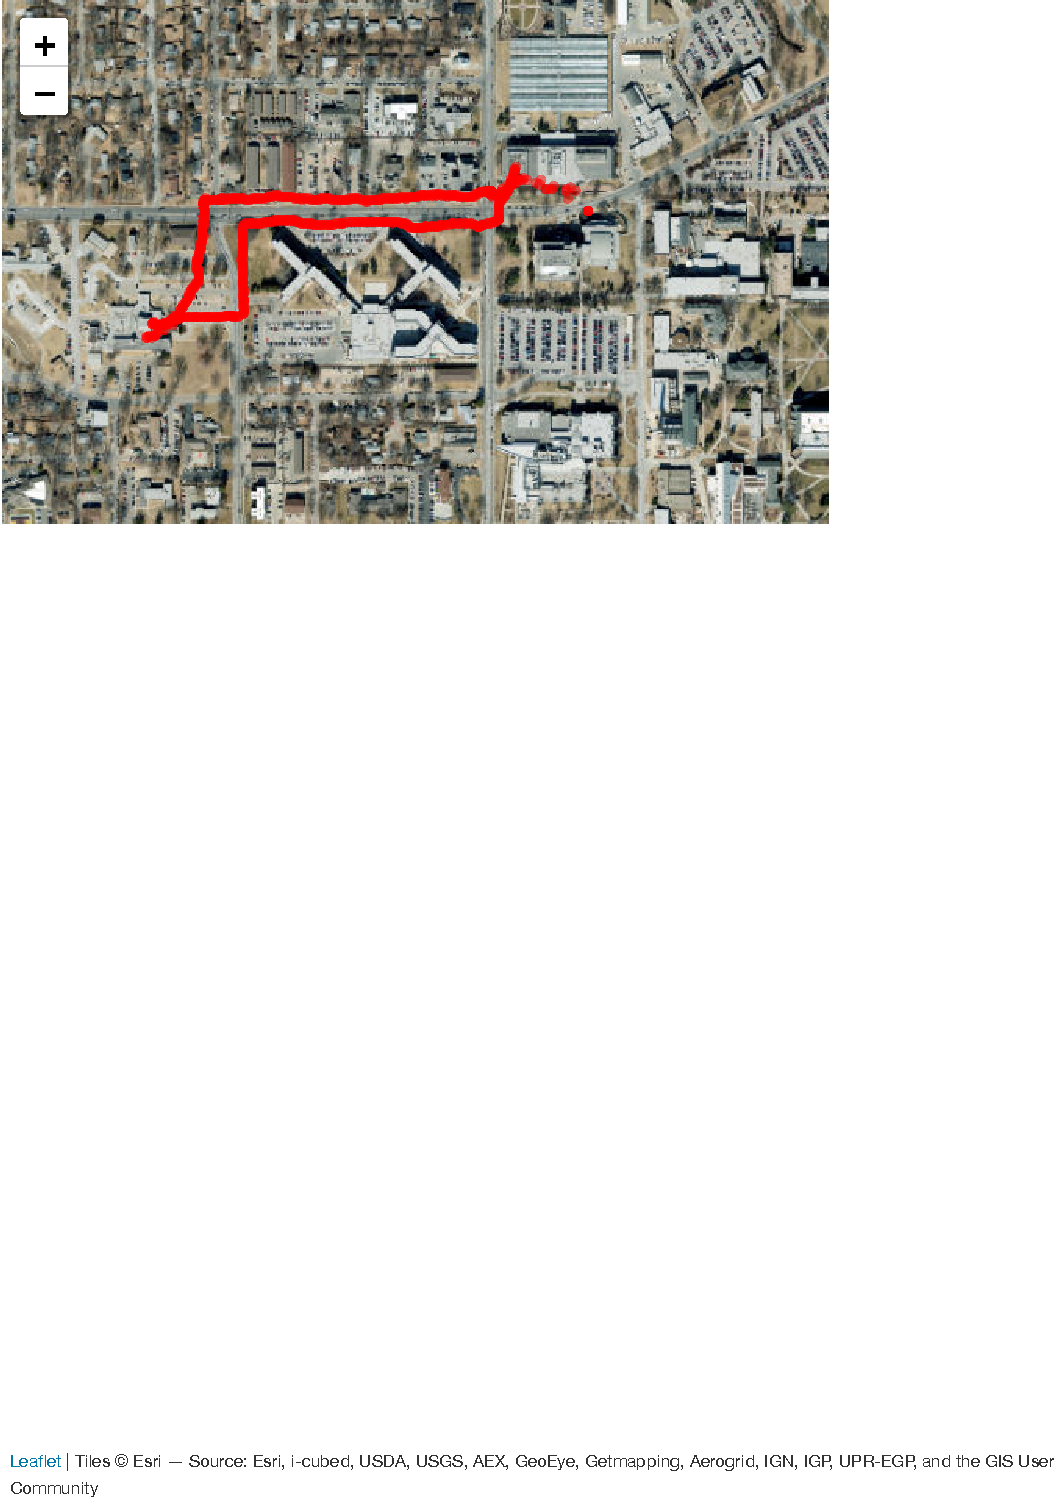
\includegraphics{_main_files/figure-latex/unnamed-chunk-3-1.pdf}

\hypertarget{write-kml}{%
\section{Write kml}\label{write-kml}}

\begin{Shaded}
\begin{Highlighting}[]
\CommentTok{\# Write to kml file to view in google earth pro}
\CommentTok{\#st\_write(am\_walk,"am\_walk.kml",driver = "kml")}

\CommentTok{\# Change date/time to class "POSIXct"}
\NormalTok{am\_walk}\SpecialCharTok{$}\NormalTok{time }\OtherTok{\textless{}{-}} \FunctionTok{as\_datetime}\NormalTok{(am\_walk}\SpecialCharTok{$}\NormalTok{time,}\AttributeTok{tz=}\StringTok{"America/Chicago"}\NormalTok{)}
\end{Highlighting}
\end{Shaded}

\hypertarget{visualize-lat-lon}{%
\section{Visualize lat lon}\label{visualize-lat-lon}}

\begin{Shaded}
\begin{Highlighting}[]
\CommentTok{\# Plot time series of spatial locations}
\FunctionTok{par}\NormalTok{(}\AttributeTok{mfrow=}\FunctionTok{c}\NormalTok{(}\DecValTok{2}\NormalTok{,}\DecValTok{1}\NormalTok{))}
\FunctionTok{plot}\NormalTok{(}\FunctionTok{data.frame}\NormalTok{(am\_walk)[[}\DecValTok{1}\NormalTok{]],}\FunctionTok{st\_coordinates}\NormalTok{(am\_walk)[,}\DecValTok{1}\NormalTok{],}\AttributeTok{pch=}\StringTok{"*"}\NormalTok{,}\AttributeTok{xlab=}\StringTok{"Time"}\NormalTok{,}\AttributeTok{ylab=}\StringTok{"Longitude"}\NormalTok{)}
\FunctionTok{plot}\NormalTok{(}\FunctionTok{data.frame}\NormalTok{(am\_walk)[[}\DecValTok{1}\NormalTok{]],}\FunctionTok{st\_coordinates}\NormalTok{(am\_walk)[,}\DecValTok{2}\NormalTok{],}\AttributeTok{pch=}\StringTok{"*"}\NormalTok{,}\AttributeTok{xlab=}\StringTok{"Time"}\NormalTok{,}\AttributeTok{ylab=}\StringTok{"Lattitude"}\NormalTok{)}
\end{Highlighting}
\end{Shaded}

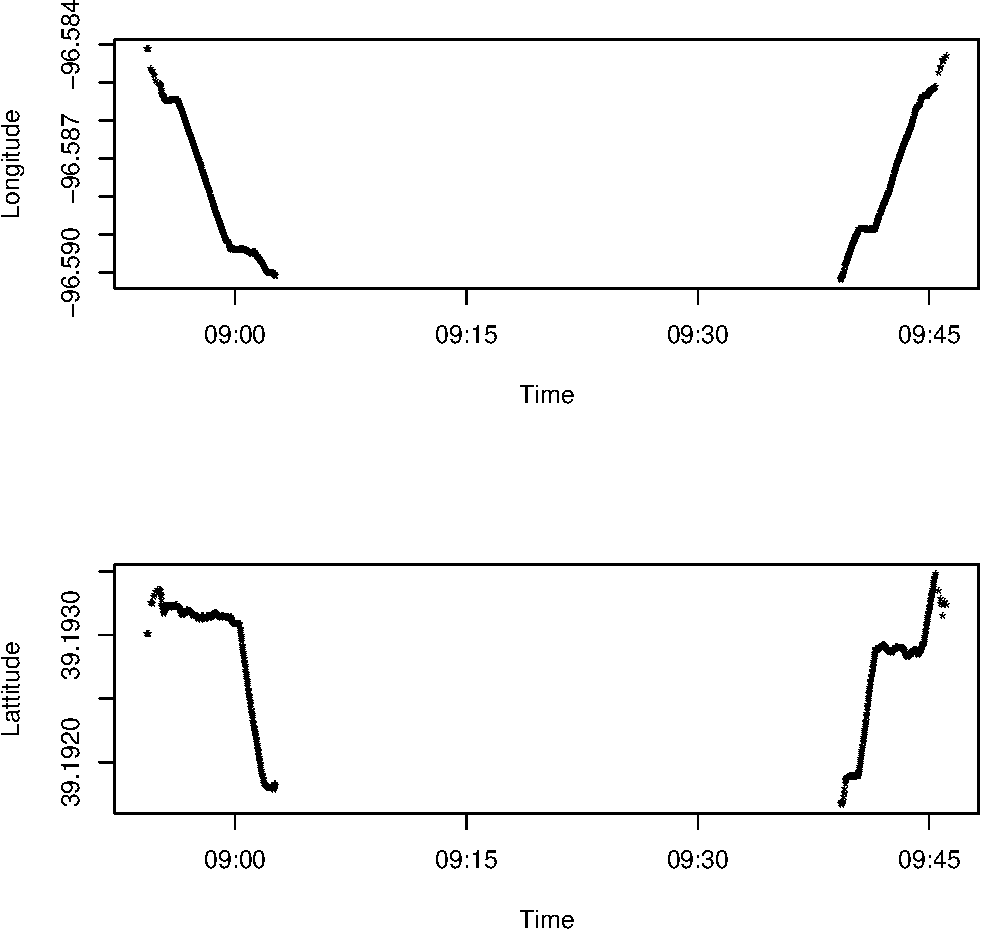
\includegraphics{_main_files/figure-latex/unnamed-chunk-5-1.pdf}

\begin{Shaded}
\begin{Highlighting}[]
\CommentTok{\# Make data.frame for data analysis}
\CommentTok{\# Note that time is in seconds since the start of the race}
\NormalTok{df.am\_walk }\OtherTok{\textless{}{-}} \FunctionTok{data.frame}\NormalTok{(}\AttributeTok{t =} \FunctionTok{as.numeric}\NormalTok{(am\_walk}\SpecialCharTok{$}\NormalTok{time }\SpecialCharTok{{-}}\NormalTok{ am\_walk}\SpecialCharTok{$}\NormalTok{time[}\DecValTok{1}\NormalTok{]),}
                          \AttributeTok{s1 =} \FunctionTok{st\_coordinates}\NormalTok{(am\_walk)[,}\DecValTok{1}\NormalTok{],}
                          \AttributeTok{s2 =} \FunctionTok{st\_coordinates}\NormalTok{(am\_walk)[,}\DecValTok{2}\NormalTok{])}
\end{Highlighting}
\end{Shaded}

\begin{Shaded}
\begin{Highlighting}[]
\FunctionTok{head}\NormalTok{(df.am\_walk)}
\end{Highlighting}
\end{Shaded}

\begin{verbatim}
##    t        s1       s2
## 1  0 -96.58411 39.19301
## 2  1 -96.58411 39.19301
## 3  5 -96.58411 39.19301
## 4  9 -96.58411 39.19301
## 5 15 -96.58463 39.19325
## 6 20 -96.58468 39.19326
\end{verbatim}

\hypertarget{polynomial}{%
\subsection{1. Polynomial}\label{polynomial}}

\begin{Shaded}
\begin{Highlighting}[]
\CommentTok{\# Fit model to longitude (s\_1) using time (t) as a predictor}
\NormalTok{m1 }\OtherTok{\textless{}{-}} \FunctionTok{lm}\NormalTok{(s1 }\SpecialCharTok{\textasciitilde{}} \FunctionTok{poly}\NormalTok{(t,}\AttributeTok{degree=}\DecValTok{10}\NormalTok{,}\AttributeTok{raw=}\ConstantTok{TRUE}\NormalTok{),}\AttributeTok{data=}\NormalTok{df.am\_walk)}

\CommentTok{\# Fit model to latitude (s\_1) using time (t) as a predictor}
\NormalTok{m2 }\OtherTok{\textless{}{-}} \FunctionTok{lm}\NormalTok{(s2 }\SpecialCharTok{\textasciitilde{}} \FunctionTok{poly}\NormalTok{(t,}\AttributeTok{degree=}\DecValTok{10}\NormalTok{,}\AttributeTok{raw=}\ConstantTok{TRUE}\NormalTok{),}\AttributeTok{data=}\NormalTok{df.am\_walk)}

\CommentTok{\# Estimate movement trajectory at a very fine temporal scale (every 1/2th of a second)}
\NormalTok{df.pred }\OtherTok{\textless{}{-}} \FunctionTok{data.frame}\NormalTok{(}\AttributeTok{t =} \FunctionTok{seq}\NormalTok{(}\DecValTok{0}\NormalTok{,}\DecValTok{3100}\NormalTok{,}\AttributeTok{by=}\FloatTok{0.5}\NormalTok{))}
\NormalTok{df.pred}\SpecialCharTok{$}\NormalTok{s1.hat }\OtherTok{\textless{}{-}} \FunctionTok{predict}\NormalTok{(m1,}\AttributeTok{newdata=}\NormalTok{df.pred)}
\NormalTok{df.pred}\SpecialCharTok{$}\NormalTok{s2.hat }\OtherTok{\textless{}{-}} \FunctionTok{predict}\NormalTok{(m2,}\AttributeTok{newdata=}\NormalTok{df.pred)}

\CommentTok{\# Plot estimated movement trajectory}
\FunctionTok{par}\NormalTok{(}\AttributeTok{mfrow=}\FunctionTok{c}\NormalTok{(}\DecValTok{2}\NormalTok{,}\DecValTok{1}\NormalTok{))}
\FunctionTok{plot}\NormalTok{(df.am\_walk}\SpecialCharTok{$}\NormalTok{t,df.am\_walk}\SpecialCharTok{$}\NormalTok{s1,}\AttributeTok{pch=}\StringTok{"*"}\NormalTok{,}\AttributeTok{xlab=}\StringTok{"Time"}\NormalTok{,}\AttributeTok{ylab=}\StringTok{"Longitude"}\NormalTok{)}
\FunctionTok{points}\NormalTok{(df.pred}\SpecialCharTok{$}\NormalTok{t,df.pred}\SpecialCharTok{$}\NormalTok{s1.hat,}\AttributeTok{typ=}\StringTok{"l"}\NormalTok{,}\AttributeTok{col=}\StringTok{"gold"}\NormalTok{,}\AttributeTok{lwd=}\DecValTok{2}\NormalTok{)}
\FunctionTok{plot}\NormalTok{(df.am\_walk}\SpecialCharTok{$}\NormalTok{t,df.am\_walk}\SpecialCharTok{$}\NormalTok{s2,}\AttributeTok{pch=}\StringTok{"*"}\NormalTok{,}\AttributeTok{xlab=}\StringTok{"Time"}\NormalTok{,}\AttributeTok{ylab=}\StringTok{"Latitude"}\NormalTok{)}
\FunctionTok{points}\NormalTok{(df.pred}\SpecialCharTok{$}\NormalTok{t,df.pred}\SpecialCharTok{$}\NormalTok{s2.hat,}\AttributeTok{typ=}\StringTok{"l"}\NormalTok{,}\AttributeTok{col=}\StringTok{"gold"}\NormalTok{,}\AttributeTok{lwd=}\DecValTok{2}\NormalTok{)}
\end{Highlighting}
\end{Shaded}

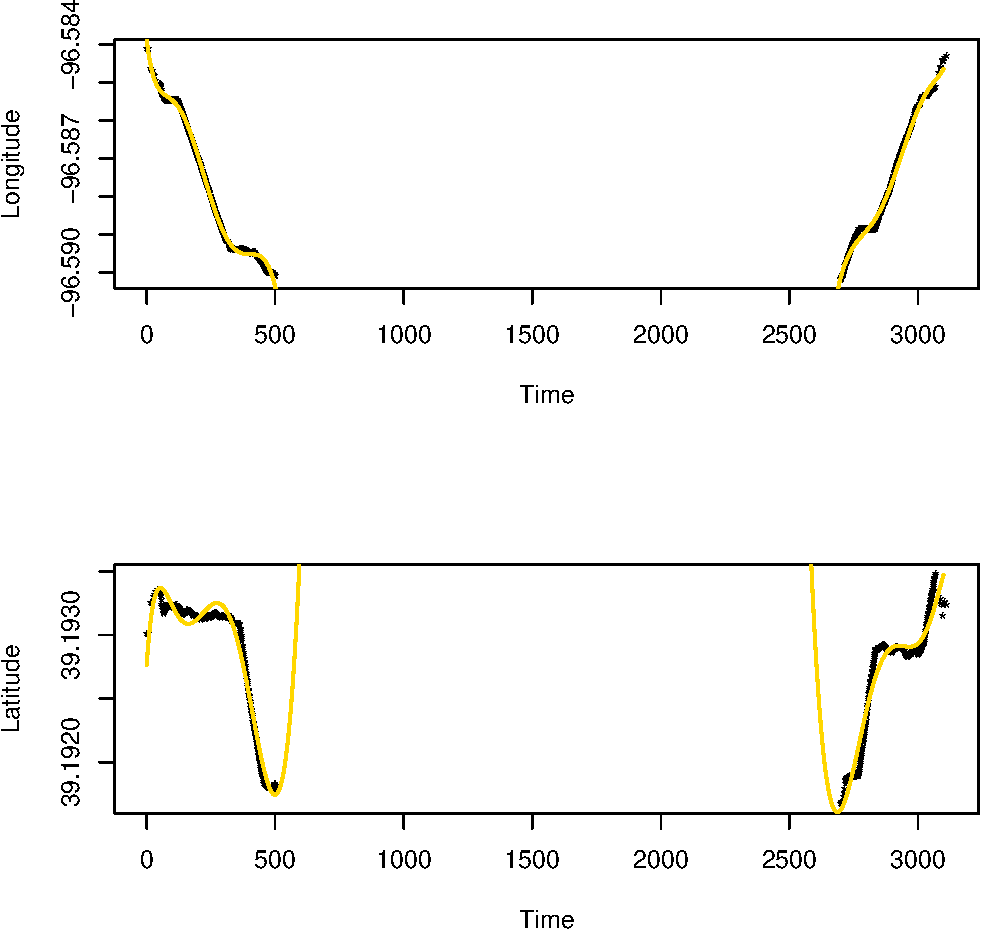
\includegraphics{_main_files/figure-latex/unnamed-chunk-7-1.pdf}

\begin{Shaded}
\begin{Highlighting}[]
\CommentTok{\# Write to kml file to view estimated trajectory in google earth pro}
\NormalTok{df.am\_walk.hat.lm }\OtherTok{\textless{}{-}} \FunctionTok{st\_as\_sf}\NormalTok{(df.pred, }\AttributeTok{coords =} \FunctionTok{c}\NormalTok{(}\StringTok{"s1.hat"}\NormalTok{, }\StringTok{"s2.hat"}\NormalTok{), }
                           \AttributeTok{crs =} \FunctionTok{st\_crs}\NormalTok{(am\_walk))}
\CommentTok{\#st\_write(df.am\_walk.hat,"am\_walk.lm.hat.kml",driver = "kml")}

\CommentTok{\# Visualize}
\NormalTok{map\_leaflet }\SpecialCharTok{\%\textgreater{}\%}
  \FunctionTok{addCircleMarkers}\NormalTok{(}\AttributeTok{data =}\NormalTok{ df.am\_walk.hat.lm,}
                   \AttributeTok{radius =} \DecValTok{3}\NormalTok{, }\AttributeTok{stroke =} \ConstantTok{FALSE}\NormalTok{, }\AttributeTok{fillOpacity =} \FloatTok{0.5}\NormalTok{,}
                   \AttributeTok{color =} \StringTok{"red"}\NormalTok{)}
\end{Highlighting}
\end{Shaded}

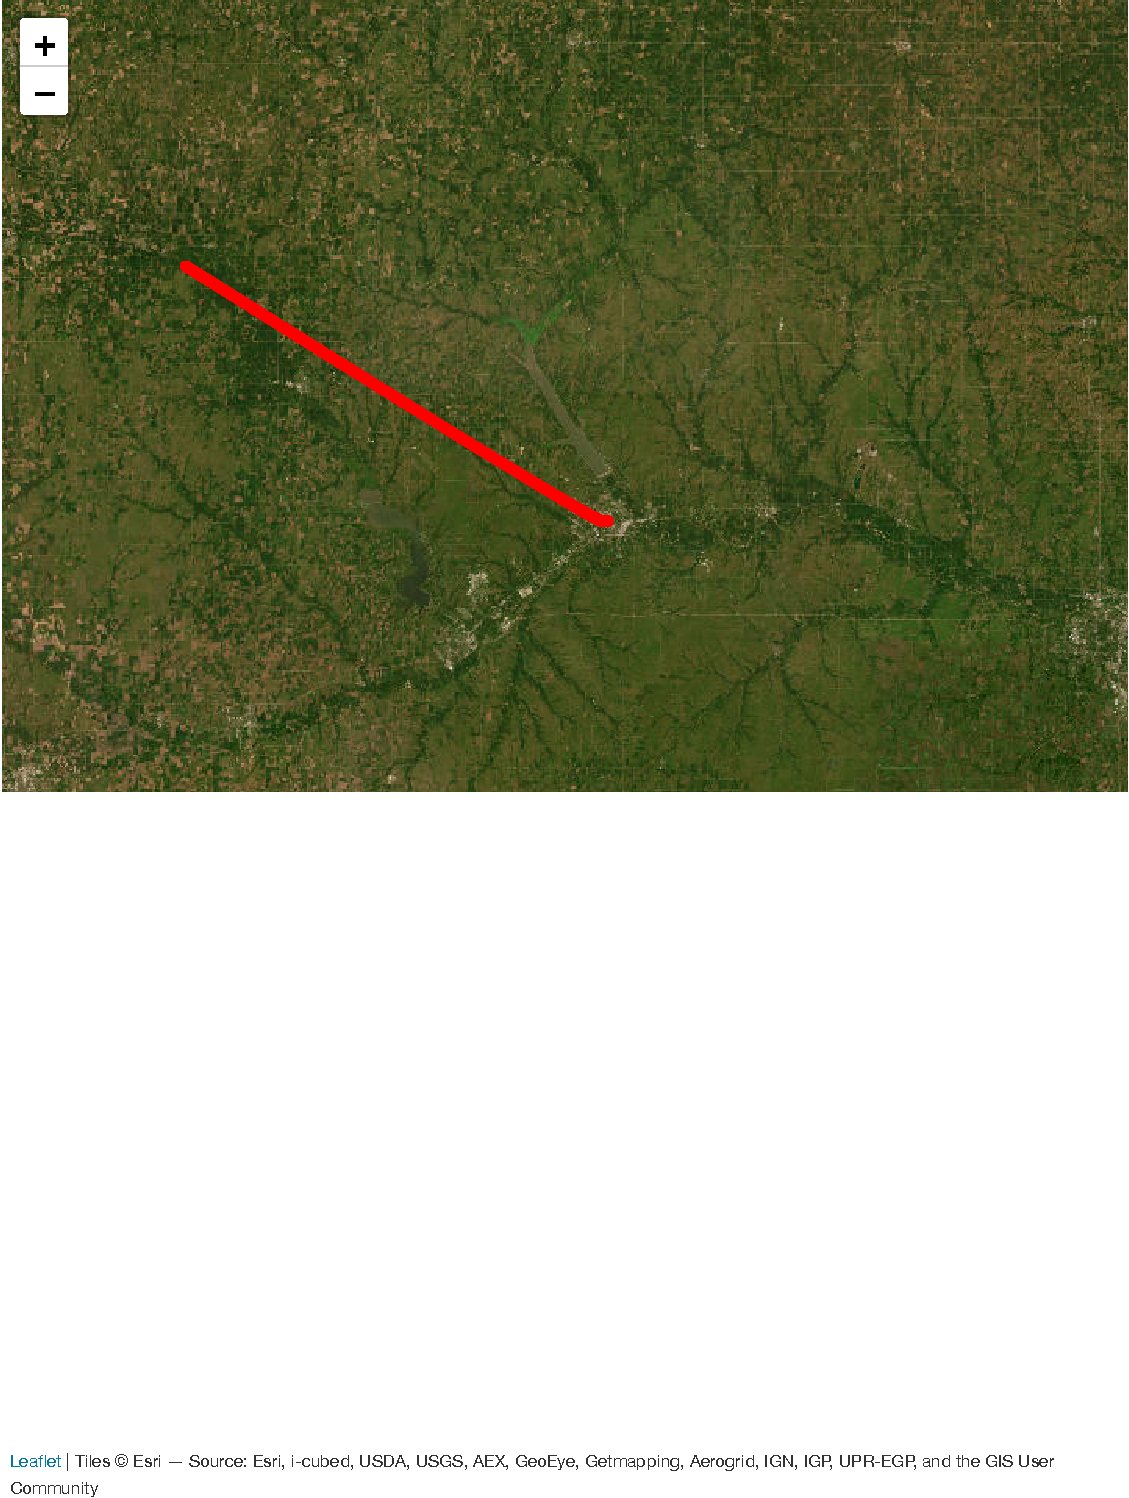
\includegraphics{_main_files/figure-latex/unnamed-chunk-7-2.pdf}

\begin{Shaded}
\begin{Highlighting}[]
\CommentTok{\# Show time series of estimated speed}
\NormalTok{dist.hat }\OtherTok{\textless{}{-}} \FunctionTok{st\_distance}\NormalTok{(df.am\_walk.hat.lm[}\DecValTok{1}\SpecialCharTok{:}\DecValTok{6200}\NormalTok{,],df.am\_walk.hat.lm[}\DecValTok{2}\SpecialCharTok{:}\DecValTok{6201}\NormalTok{,],}\AttributeTok{by\_element=}\ConstantTok{TRUE}\NormalTok{)}
\NormalTok{(}\FunctionTok{sum}\NormalTok{(dist.hat)}\SpecialCharTok{/}\DecValTok{1000}\NormalTok{)}\SpecialCharTok{*}\FloatTok{0.62} \CommentTok{\# Model check. Length of estimated trajectory in miles}
\end{Highlighting}
\end{Shaded}

\begin{verbatim}
## 92.95302 [m]
\end{verbatim}

\begin{Shaded}
\begin{Highlighting}[]
\NormalTok{speed.hat }\OtherTok{\textless{}{-}}\NormalTok{ (dist.hat}\SpecialCharTok{/}\FloatTok{0.5}\NormalTok{)}\SpecialCharTok{*}\FloatTok{2.24} \CommentTok{\# units are in miles per hour}
\FunctionTok{plot}\NormalTok{(df.pred}\SpecialCharTok{$}\NormalTok{t[}\SpecialCharTok{{-}}\DecValTok{1}\NormalTok{],speed.hat,}\AttributeTok{xlab=}\StringTok{"Time (seconds)"}\NormalTok{,}\AttributeTok{ylab=}\StringTok{"Velocity (miles per hour)"}\NormalTok{)}

\CommentTok{\# Comparison to observed data}
\CommentTok{\# Class discussion about what would happen if we collected more location data?}
\NormalTok{dist }\OtherTok{\textless{}{-}} \FunctionTok{st\_distance}\NormalTok{(am\_walk[}\DecValTok{1}\SpecialCharTok{:}\DecValTok{840}\NormalTok{,],am\_walk[}\DecValTok{2}\SpecialCharTok{:}\DecValTok{841}\NormalTok{,],}\AttributeTok{by\_element=}\ConstantTok{TRUE}\NormalTok{)}
\NormalTok{(}\FunctionTok{sum}\NormalTok{(dist, }\AttributeTok{na.rm =}\NormalTok{ T)}\SpecialCharTok{/}\DecValTok{1000}\NormalTok{)}\SpecialCharTok{*}\FloatTok{0.62}
\end{Highlighting}
\end{Shaded}

\begin{verbatim}
## 0.8918068 [m]
\end{verbatim}

\begin{Shaded}
\begin{Highlighting}[]
\NormalTok{speed }\OtherTok{\textless{}{-}}\NormalTok{ (dist}\SpecialCharTok{/}\FunctionTok{as.numeric}\NormalTok{(}\FunctionTok{diff}\NormalTok{(am\_walk}\SpecialCharTok{$}\NormalTok{time)))}\SpecialCharTok{*}\FloatTok{2.24}
\end{Highlighting}
\end{Shaded}

\begin{verbatim}
## Warning in `/.default`(dist, as.numeric(diff(am_walk$time))): longer object
## length is not a multiple of shorter object length
\end{verbatim}

\begin{Shaded}
\begin{Highlighting}[]
\FunctionTok{plot}\NormalTok{(df.am\_walk}\SpecialCharTok{$}\NormalTok{t,speed,}\AttributeTok{xlab=}\StringTok{"Time (seconds)"}\NormalTok{,}\AttributeTok{ylab=}\StringTok{"Velocity (miles per hour)"}\NormalTok{)}
\end{Highlighting}
\end{Shaded}

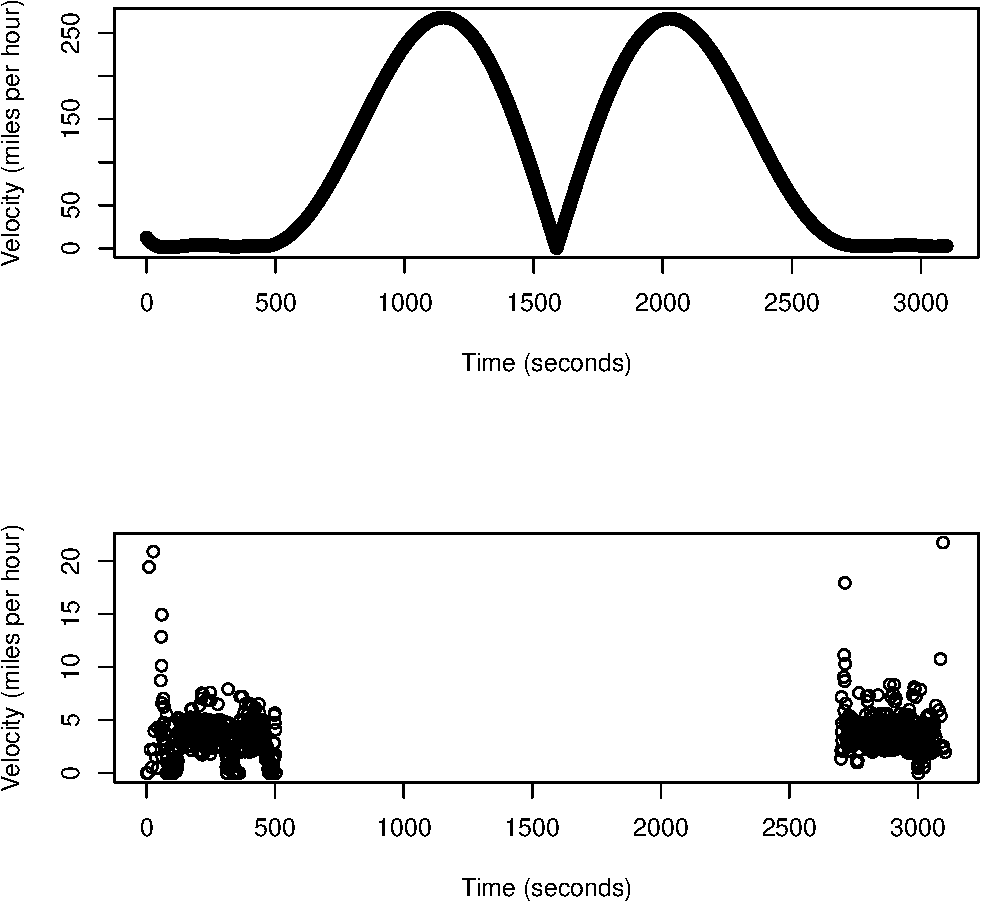
\includegraphics{_main_files/figure-latex/unnamed-chunk-7-3.pdf}

\hypertarget{gam---low-rank-gaussian-process}{%
\subsection{2. GAM - low rank gaussian process}\label{gam---low-rank-gaussian-process}}

\begin{Shaded}
\begin{Highlighting}[]
\CommentTok{\# Fit model to longitude (s\_1) using time (t) as a predictor}
\NormalTok{m1 }\OtherTok{\textless{}{-}} \FunctionTok{gam}\NormalTok{(s1 }\SpecialCharTok{\textasciitilde{}} \FunctionTok{s}\NormalTok{(t,}\AttributeTok{bs=}\StringTok{"gp"}\NormalTok{,}\AttributeTok{k=}\DecValTok{50}\NormalTok{),}\AttributeTok{data=}\NormalTok{df.am\_walk)}

\CommentTok{\# Fit model to latitude (s\_1) using time (t) as a predictor}
\NormalTok{m2 }\OtherTok{\textless{}{-}} \FunctionTok{gam}\NormalTok{(s2 }\SpecialCharTok{\textasciitilde{}} \FunctionTok{s}\NormalTok{(t,}\AttributeTok{bs=}\StringTok{"gp"}\NormalTok{,}\AttributeTok{k=}\DecValTok{50}\NormalTok{),}\AttributeTok{data=}\NormalTok{df.am\_walk)}

\CommentTok{\# Estimate movement trajectory at a very fine temporal scale (every 1/2th of a second)}
\NormalTok{df.pred }\OtherTok{\textless{}{-}} \FunctionTok{data.frame}\NormalTok{(}\AttributeTok{t =} \FunctionTok{seq}\NormalTok{(}\DecValTok{0}\NormalTok{,}\DecValTok{3100}\NormalTok{,}\AttributeTok{by=}\FloatTok{0.5}\NormalTok{))}
\NormalTok{df.pred}\SpecialCharTok{$}\NormalTok{s1.hat }\OtherTok{\textless{}{-}} \FunctionTok{predict}\NormalTok{(m1,}\AttributeTok{newdata=}\NormalTok{df.pred)}
\NormalTok{df.pred}\SpecialCharTok{$}\NormalTok{s2.hat }\OtherTok{\textless{}{-}} \FunctionTok{predict}\NormalTok{(m2,}\AttributeTok{newdata=}\NormalTok{df.pred)}

\CommentTok{\# Plot estimated movement trajectory}
\FunctionTok{par}\NormalTok{(}\AttributeTok{mfrow=}\FunctionTok{c}\NormalTok{(}\DecValTok{2}\NormalTok{,}\DecValTok{1}\NormalTok{))}
\FunctionTok{plot}\NormalTok{(df.am\_walk}\SpecialCharTok{$}\NormalTok{t,df.am\_walk}\SpecialCharTok{$}\NormalTok{s1,}\AttributeTok{pch=}\StringTok{"*"}\NormalTok{,}\AttributeTok{xlab=}\StringTok{"Time"}\NormalTok{,}\AttributeTok{ylab=}\StringTok{"Longitude"}\NormalTok{)}
\FunctionTok{points}\NormalTok{(df.pred}\SpecialCharTok{$}\NormalTok{t,df.pred}\SpecialCharTok{$}\NormalTok{s1.hat,}\AttributeTok{typ=}\StringTok{"l"}\NormalTok{,}\AttributeTok{col=}\StringTok{"gold"}\NormalTok{,}\AttributeTok{lwd=}\DecValTok{2}\NormalTok{)}
\FunctionTok{plot}\NormalTok{(df.am\_walk}\SpecialCharTok{$}\NormalTok{t,df.am\_walk}\SpecialCharTok{$}\NormalTok{s2,}\AttributeTok{pch=}\StringTok{"*"}\NormalTok{,}\AttributeTok{xlab=}\StringTok{"Time"}\NormalTok{,}\AttributeTok{ylab=}\StringTok{"Latitude"}\NormalTok{)}
\FunctionTok{points}\NormalTok{(df.pred}\SpecialCharTok{$}\NormalTok{t,df.pred}\SpecialCharTok{$}\NormalTok{s2.hat,}\AttributeTok{typ=}\StringTok{"l"}\NormalTok{,}\AttributeTok{col=}\StringTok{"gold"}\NormalTok{,}\AttributeTok{lwd=}\DecValTok{2}\NormalTok{)}
\end{Highlighting}
\end{Shaded}

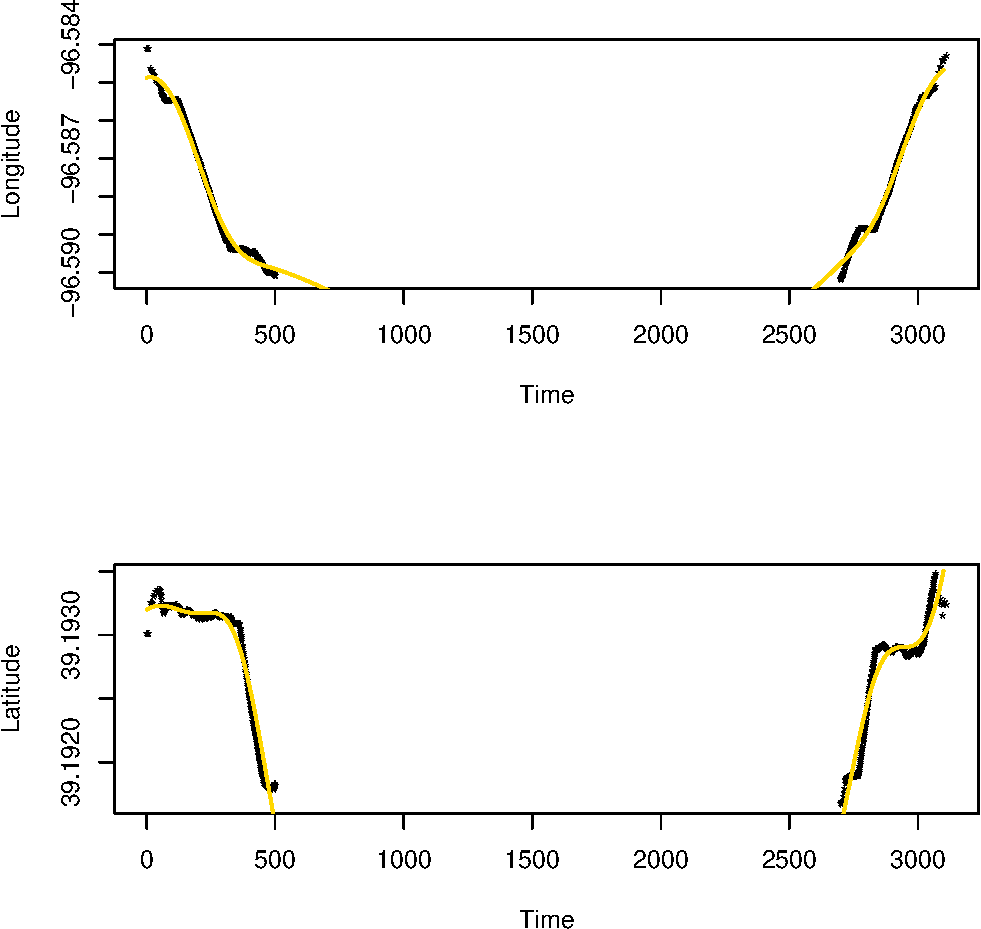
\includegraphics{_main_files/figure-latex/unnamed-chunk-8-1.pdf}

\begin{Shaded}
\begin{Highlighting}[]
\CommentTok{\# Write to kml file to view estimated trajectory in google earth pro}
\NormalTok{df.am\_walk.hat.gam }\OtherTok{\textless{}{-}} \FunctionTok{st\_as\_sf}\NormalTok{(df.pred, }\AttributeTok{coords =} \FunctionTok{c}\NormalTok{(}\StringTok{"s1.hat"}\NormalTok{, }\StringTok{"s2.hat"}\NormalTok{), }
                           \AttributeTok{crs =} \FunctionTok{st\_crs}\NormalTok{(am\_walk))}
\CommentTok{\#st\_write(df.am\_walk.hat,"am\_walk.gam.hat.kml",driver = "kml")}

\CommentTok{\# Visualize}
\NormalTok{map\_leaflet }\SpecialCharTok{\%\textgreater{}\%}
  \FunctionTok{addCircleMarkers}\NormalTok{(}\AttributeTok{data =}\NormalTok{ df.am\_walk.hat.gam,}
                   \AttributeTok{radius =} \DecValTok{3}\NormalTok{, }\AttributeTok{stroke =} \ConstantTok{FALSE}\NormalTok{, }\AttributeTok{fillOpacity =} \FloatTok{0.5}\NormalTok{,}
                   \AttributeTok{color =} \StringTok{"red"}\NormalTok{)}
\end{Highlighting}
\end{Shaded}

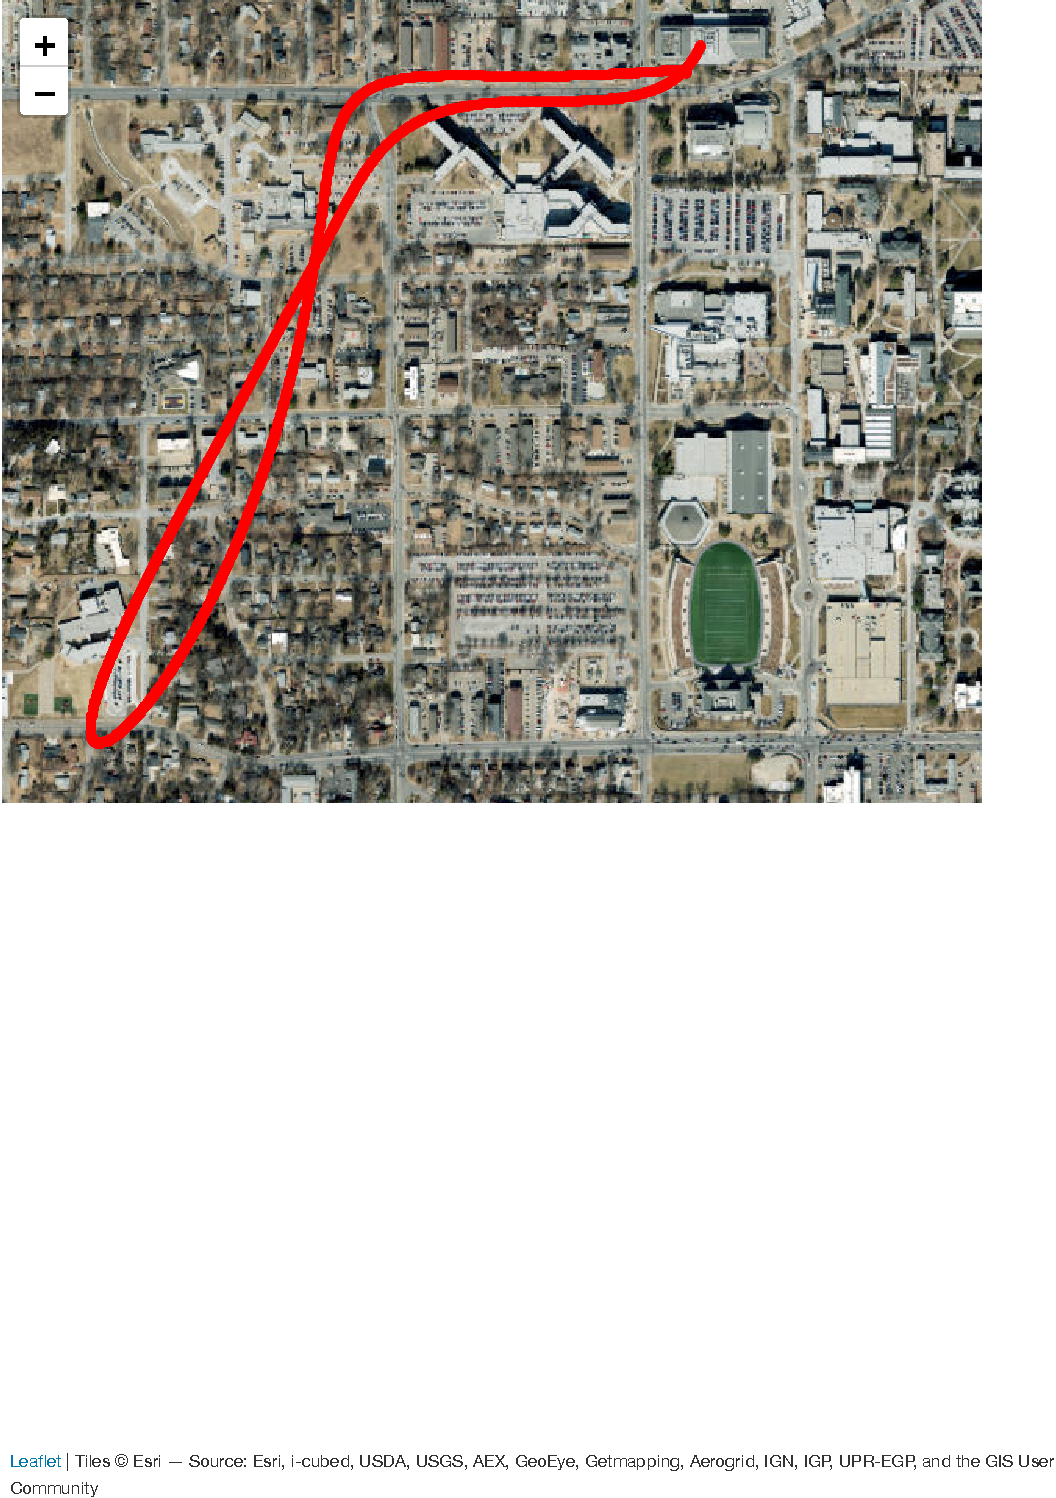
\includegraphics{_main_files/figure-latex/unnamed-chunk-8-2.pdf}

\begin{Shaded}
\begin{Highlighting}[]
\CommentTok{\# Show time series of estimated speed}
\NormalTok{dist.hat }\OtherTok{\textless{}{-}} \FunctionTok{st\_distance}\NormalTok{(df.am\_walk.hat.gam[}\DecValTok{1}\SpecialCharTok{:}\DecValTok{6200}\NormalTok{,],df.am\_walk.hat.gam[}\DecValTok{2}\SpecialCharTok{:}\DecValTok{6201}\NormalTok{,],}\AttributeTok{by\_element=}\ConstantTok{TRUE}\NormalTok{)}
\NormalTok{(}\FunctionTok{sum}\NormalTok{(dist.hat)}\SpecialCharTok{/}\DecValTok{1000}\NormalTok{)}\SpecialCharTok{*}\FloatTok{0.62} \CommentTok{\# Model check. Length of estimated trajectory in miles. Should be \textasciitilde{}26.2}
\end{Highlighting}
\end{Shaded}

\begin{verbatim}
## 1.519816 [m]
\end{verbatim}

\begin{Shaded}
\begin{Highlighting}[]
\NormalTok{speed.hat }\OtherTok{\textless{}{-}}\NormalTok{ (dist.hat}\SpecialCharTok{/}\FloatTok{0.5}\NormalTok{)}\SpecialCharTok{*}\FloatTok{2.24} \CommentTok{\# units are in miles per hour}
\FunctionTok{plot}\NormalTok{(df.pred}\SpecialCharTok{$}\NormalTok{t[}\SpecialCharTok{{-}}\DecValTok{1}\NormalTok{],speed.hat,}\AttributeTok{xlab=}\StringTok{"Time (seconds)"}\NormalTok{,}\AttributeTok{ylab=}\StringTok{"Velocity (miles per hour)"}\NormalTok{)}

\CommentTok{\# Comparison to observed data}
\CommentTok{\# Class discussion about what would happen if we collected more location data?}
\NormalTok{dist }\OtherTok{\textless{}{-}} \FunctionTok{st\_distance}\NormalTok{(am\_walk[}\DecValTok{1}\SpecialCharTok{:}\DecValTok{840}\NormalTok{,],am\_walk[}\DecValTok{2}\SpecialCharTok{:}\DecValTok{841}\NormalTok{,],}\AttributeTok{by\_element=}\ConstantTok{TRUE}\NormalTok{)}
\NormalTok{(}\FunctionTok{sum}\NormalTok{(dist, }\AttributeTok{na.rm =}\NormalTok{ T)}\SpecialCharTok{/}\DecValTok{1000}\NormalTok{)}\SpecialCharTok{*}\FloatTok{0.62}
\end{Highlighting}
\end{Shaded}

\begin{verbatim}
## 0.8918068 [m]
\end{verbatim}

\begin{Shaded}
\begin{Highlighting}[]
\NormalTok{speed }\OtherTok{\textless{}{-}}\NormalTok{ (dist}\SpecialCharTok{/}\FunctionTok{as.numeric}\NormalTok{(}\FunctionTok{diff}\NormalTok{(am\_walk}\SpecialCharTok{$}\NormalTok{time)))}\SpecialCharTok{*}\FloatTok{2.24}
\end{Highlighting}
\end{Shaded}

\begin{verbatim}
## Warning in `/.default`(dist, as.numeric(diff(am_walk$time))): longer object
## length is not a multiple of shorter object length
\end{verbatim}

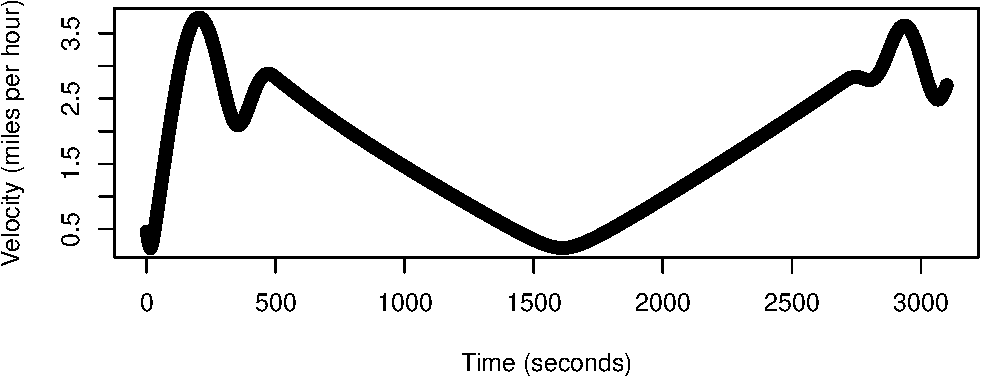
\includegraphics{_main_files/figure-latex/unnamed-chunk-8-3.pdf}

\hypertarget{regression-tree}{%
\subsection{3. Regression tree}\label{regression-tree}}

\begin{Shaded}
\begin{Highlighting}[]
\CommentTok{\# Fit model to longitude (s\_1) using time (t) as a predictor}
\NormalTok{m1 }\OtherTok{\textless{}{-}} \FunctionTok{rpart}\NormalTok{(s1 }\SpecialCharTok{\textasciitilde{}}\NormalTok{ t,}\AttributeTok{data=}\NormalTok{df.am\_walk,}\AttributeTok{control=}\FunctionTok{rpart.control}\NormalTok{(}\AttributeTok{cp =} \FloatTok{0.0001}\NormalTok{))}
\FunctionTok{summary}\NormalTok{(m1)}
\end{Highlighting}
\end{Shaded}

\begin{verbatim}
## Call:
## rpart(formula = s1 ~ t, data = df.am_walk, control = rpart.control(cp = 1e-04))
##   n= 840 
## 
##              CP nsplit   rel error      xerror         xstd
## 1  0.4038325880      0 1.000000000 1.002492526 0.0276603288
## 2  0.0529333038      2 0.192334824 0.197130137 0.0086257627
## 3  0.0382549078      3 0.139401520 0.136601803 0.0063549591
## 4  0.0313627583      4 0.101146612 0.103532021 0.0052777010
## 5  0.0173229189      5 0.069783854 0.070204005 0.0036158948
## 6  0.0098997579      6 0.052460935 0.052551512 0.0026895564
## 7  0.0085011146      7 0.042561177 0.044194161 0.0024759007
## 8  0.0038495110      8 0.034060063 0.035206291 0.0020794139
## 9  0.0035614160      9 0.030210552 0.033289418 0.0020483808
## 10 0.0034149717     10 0.026649136 0.028642049 0.0018541217
## 11 0.0033040808     12 0.019819192 0.028264732 0.0018510619
## 12 0.0027800834     13 0.016515112 0.019144325 0.0015618568
## 13 0.0017319532     14 0.013735028 0.015302724 0.0008741446
## 14 0.0016226090     15 0.012003075 0.014135906 0.0007958051
## 15 0.0010277729     16 0.010380466 0.011844197 0.0006606555
## 16 0.0009213428     17 0.009352693 0.010852983 0.0006047498
## 17 0.0006320311     18 0.008431350 0.009852370 0.0005738556
## 18 0.0005726033     19 0.007799319 0.009245986 0.0005529182
## 19 0.0005239639     20 0.007226716 0.008775950 0.0005402320
## 20 0.0005013861     21 0.006702752 0.008373828 0.0005313339
## 21 0.0004641290     22 0.006201366 0.007546584 0.0005121934
## 22 0.0004338286     23 0.005737237 0.006943036 0.0004949454
## 23 0.0004166754     24 0.005303408 0.006342352 0.0004778446
## 24 0.0003996006     25 0.004886733 0.006143846 0.0004742798
## 25 0.0003684265     26 0.004487132 0.005636062 0.0004602969
## 26 0.0002634018     27 0.004118706 0.005174283 0.0004427461
## 27 0.0002112131     28 0.003855304 0.004715714 0.0004328984
## 28 0.0001966654     29 0.003644091 0.004574930 0.0004280876
## 29 0.0001773506     30 0.003447426 0.004392472 0.0004251736
## 30 0.0001519357     31 0.003270075 0.004082797 0.0004217902
## 31 0.0001454195     32 0.003118139 0.003911566 0.0004194165
## 32 0.0001205736     33 0.002972720 0.003809751 0.0004185487
## 33 0.0001125103     34 0.002852146 0.003696916 0.0004164463
## 34 0.0001122899     35 0.002739636 0.003660828 0.0004164494
## 35 0.0001000000     36 0.002627346 0.003557704 0.0004138635
## 
## Variable importance
##   t 
## 100 
## 
## Node number 1: 840 observations,    complexity param=0.4038326
##   mean=-96.58774, MSE=2.874721e-06 
##   left son=2 (680 obs) right son=3 (160 obs)
##   Primary splits:
##       t < 200.5  to the right, improve=0.3240044, (0 missing)
## 
## Node number 2: 680 observations,    complexity param=0.4038326
##   mean=-96.58821, MSE=2.312706e-06 
##   left son=4 (511 obs) right son=5 (169 obs)
##   Primary splits:
##       t < 2908.5 to the left,  improve=0.7426539, (0 missing)
## 
## Node number 3: 160 observations,    complexity param=0.01732292
##   mean=-96.58575, MSE=3.733175e-07 
##   left son=6 (55 obs) right son=7 (105 obs)
##   Primary splits:
##       t < 145.5  to the right, improve=0.7003219, (0 missing)
## 
## Node number 4: 511 observations,    complexity param=0.0529333
##   mean=-96.58896, MSE=5.985343e-07 
##   left son=8 (441 obs) right son=9 (70 obs)
##   Primary splits:
##       t < 270.5  to the right, improve=0.4179209, (0 missing)
## 
## Node number 5: 169 observations,    complexity param=0.03136276
##   mean=-96.58593, MSE=5.849805e-07 
##   left son=10 (72 obs) right son=11 (97 obs)
##   Primary splits:
##       t < 2980.5 to the left,  improve=0.7660571, (0 missing)
## 
## Node number 6: 55 observations,    complexity param=0.001622609
##   mean=-96.58646, MSE=9.504505e-08 
##   left son=12 (27 obs) right son=13 (28 obs)
##   Primary splits:
##       t < 173.5  to the right, improve=0.7495432, (0 missing)
## 
## Node number 7: 105 observations,    complexity param=0.003561416
##   mean=-96.58538, MSE=1.206908e-07 
##   left son=14 (90 obs) right son=15 (15 obs)
##   Primary splits:
##       t < 55.5   to the right, improve=0.6786316, (0 missing)
## 
## Node number 8: 441 observations,    complexity param=0.03825491
##   mean=-96.58916, MSE=3.754649e-07 
##   left son=16 (298 obs) right son=17 (143 obs)
##   Primary splits:
##       t < 2765.5 to the left,  improve=0.5578973, (0 missing)
## 
## Node number 9: 70 observations,    complexity param=0.003849511
##   mean=-96.58771, MSE=1.778497e-07 
##   left son=18 (34 obs) right son=19 (36 obs)
##   Primary splits:
##       t < 236.5  to the right, improve=0.746671, (0 missing)
## 
## Node number 10: 72 observations,    complexity param=0.003304081
##   mean=-96.5867, MSE=1.489385e-07 
##   left son=20 (34 obs) right son=21 (38 obs)
##   Primary splits:
##       t < 2942.5 to the left,  improve=0.7440225, (0 missing)
## 
## Node number 11: 97 observations,    complexity param=0.002780083
##   mean=-96.58535, MSE=1.278806e-07 
##   left son=22 (89 obs) right son=23 (8 obs)
##   Primary splits:
##       t < 3076   to the left,  improve=0.5411983, (0 missing)
## 
## Node number 12: 27 observations,    complexity param=0.0001966654
##   mean=-96.58673, MSE=2.314742e-08 
##   left son=24 (13 obs) right son=25 (14 obs)
##   Primary splits:
##       t < 187.5  to the right, improve=0.7598653, (0 missing)
## 
## Node number 13: 28 observations,    complexity param=0.0002112131
##   mean=-96.58619, MSE=2.443846e-08 
##   left son=26 (14 obs) right son=27 (14 obs)
##   Primary splits:
##       t < 159.5  to the right, improve=0.7453561, (0 missing)
## 
## Node number 14: 90 observations,    complexity param=0.0005726033
##   mean=-96.5855, MSE=2.260186e-08 
##   left son=28 (17 obs) right son=29 (73 obs)
##   Primary splits:
##       t < 128.5  to the right, improve=0.679739, (0 missing)
## 
## Node number 15: 15 observations
##   mean=-96.58468, MSE=1.358924e-07 
## 
## Node number 16: 298 observations,    complexity param=0.008501115
##   mean=-96.58948, MSE=1.48135e-07 
##   left son=32 (249 obs) right son=33 (49 obs)
##   Primary splits:
##       t < 319.5  to the right, improve=0.4650255, (0 missing)
## 
## Node number 17: 143 observations,    complexity param=0.009899758
##   mean=-96.5885, MSE=2.032107e-07 
##   left son=34 (94 obs) right son=35 (49 obs)
##   Primary splits:
##       t < 2859.5 to the left,  improve=0.8226535, (0 missing)
## 
## Node number 18: 34 observations,    complexity param=0.000464129
##   mean=-96.58808, MSE=4.365118e-08 
##   left son=36 (17 obs) right son=37 (17 obs)
##   Primary splits:
##       t < 253.5  to the right, improve=0.7551595, (0 missing)
## 
## Node number 19: 36 observations,    complexity param=0.0005239639
##   mean=-96.58735, MSE=4.637986e-08 
##   left son=38 (18 obs) right son=39 (18 obs)
##   Primary splits:
##       t < 218.5  to the right, improve=0.7577822, (0 missing)
## 
## Node number 20: 34 observations,    complexity param=0.0004338286
##   mean=-96.58706, MSE=4.089916e-08 
##   left son=40 (16 obs) right son=41 (18 obs)
##   Primary splits:
##       t < 2924.5 to the left,  improve=0.7533552, (0 missing)
## 
## Node number 21: 38 observations,    complexity param=0.0004166754
##   mean=-96.58639, MSE=3.56427e-08 
##   left son=42 (20 obs) right son=43 (18 obs)
##   Primary splits:
##       t < 2962.5 to the left,  improve=0.7428798, (0 missing)
## 
## Node number 22: 89 observations,    complexity param=0.001731953
##   mean=-96.58543, MSE=6.200105e-08 
##   left son=44 (32 obs) right son=45 (57 obs)
##   Primary splits:
##       t < 3012.5 to the left,  improve=0.7579178, (0 missing)
## 
## Node number 23: 8 observations
##   mean=-96.58447, MSE=2.163419e-08 
## 
## Node number 24: 13 observations
##   mean=-96.58687, MSE=4.994154e-09 
## 
## Node number 25: 14 observations
##   mean=-96.5866, MSE=6.082531e-09 
## 
## Node number 26: 14 observations
##   mean=-96.58633, MSE=6.041245e-09 
## 
## Node number 27: 14 observations
##   mean=-96.58606, MSE=6.404964e-09 
## 
## Node number 28: 17 observations
##   mean=-96.58575, MSE=9.083855e-09 
## 
## Node number 29: 73 observations,    complexity param=0.0001519357
##   mean=-96.58544, MSE=6.808752e-09 
##   left son=58 (63 obs) right son=59 (10 obs)
##   Primary splits:
##       t < 65.5   to the right, improve=0.7381497, (0 missing)
## 
## Node number 32: 249 observations,    complexity param=0.003414972
##   mean=-96.58959, MSE=8.334358e-08 
##   left son=64 (136 obs) right son=65 (113 obs)
##   Primary splits:
##       t < 432.5  to the right, improve=0.2947253, (0 missing)
## 
## Node number 33: 49 observations,    complexity param=0.0009213428
##   mean=-96.58889, MSE=5.843859e-08 
##   left son=66 (26 obs) right son=67 (23 obs)
##   Primary splits:
##       t < 293.5  to the right, improve=0.7769632, (0 missing)
## 
## Node number 34: 94 observations,    complexity param=0.0006320311
##   mean=-96.58879, MSE=1.912901e-08 
##   left son=68 (78 obs) right son=69 (16 obs)
##   Primary splits:
##       t < 2843.5 to the left,  improve=0.848776, (0 missing)
## 
## Node number 35: 49 observations,    complexity param=0.001027773
##   mean=-96.58793, MSE=6.847773e-08 
##   left son=70 (28 obs) right son=71 (21 obs)
##   Primary splits:
##       t < 2887.5 to the left,  improve=0.7396508, (0 missing)
## 
## Node number 36: 17 observations
##   mean=-96.58826, MSE=1.047421e-08 
## 
## Node number 37: 17 observations
##   mean=-96.5879, MSE=1.090095e-08 
## 
## Node number 38: 18 observations
##   mean=-96.58754, MSE=1.118114e-08 
## 
## Node number 39: 18 observations
##   mean=-96.58716, MSE=1.128691e-08 
## 
## Node number 40: 16 observations
##   mean=-96.58724, MSE=1.054293e-08 
## 
## Node number 41: 18 observations
##   mean=-96.58689, MSE=9.682793e-09 
## 
## Node number 42: 20 observations
##   mean=-96.58654, MSE=9.784048e-09 
## 
## Node number 43: 18 observations
##   mean=-96.58622, MSE=8.476025e-09 
## 
## Node number 44: 32 observations,    complexity param=0.0002634018
##   mean=-96.58572, MSE=2.486718e-08 
##   left son=88 (12 obs) right son=89 (20 obs)
##   Primary splits:
##       t < 2992.5 to the left,  improve=0.7993136, (0 missing)
## 
## Node number 45: 57 observations,    complexity param=0.0001773506
##   mean=-96.58527, MSE=9.475135e-09 
##   left son=90 (32 obs) right son=91 (25 obs)
##   Primary splits:
##       t < 3044.5 to the left,  improve=0.7929531, (0 missing)
## 
## Node number 58: 63 observations
##   mean=-96.58546, MSE=9.714104e-10 
## 
## Node number 59: 10 observations
##   mean=-96.58526, MSE=6.89509e-09 
## 
## Node number 64: 136 observations,    complexity param=0.003414972
##   mean=-96.58974, MSE=1.047554e-07 
##   left son=128 (101 obs) right son=129 (35 obs)
##   Primary splits:
##       t < 2730.5 to the left,  improve=0.7283357, (0 missing)
## 
## Node number 65: 113 observations,    complexity param=0.0001122899
##   mean=-96.58942, MSE=3.446993e-09 
##   left son=130 (42 obs) right son=131 (71 obs)
##   Primary splits:
##       t < 390.5  to the right, improve=0.6961402, (0 missing)
## 
## Node number 66: 26 observations
##   mean=-96.58909, MSE=1.031009e-08 
## 
## Node number 67: 23 observations,    complexity param=0.0001125103
##   mean=-96.58866, MSE=1.611311e-08 
##   left son=134 (12 obs) right son=135 (11 obs)
##   Primary splits:
##       t < 281.5  to the right, improve=0.7330945, (0 missing)
## 
## Node number 68: 78 observations
##   mean=-96.58885, MSE=1.865192e-09 
## 
## Node number 69: 16 observations
##   mean=-96.58851, MSE=7.902184e-09 
## 
## Node number 70: 28 observations,    complexity param=0.0001454195
##   mean=-96.58813, MSE=1.730372e-08 
##   left son=140 (15 obs) right son=141 (13 obs)
##   Primary splits:
##       t < 2874.5 to the left,  improve=0.7247701, (0 missing)
## 
## Node number 71: 21 observations,    complexity param=0.0001205736
##   mean=-96.58767, MSE=1.852732e-08 
##   left son=142 (10 obs) right son=143 (11 obs)
##   Primary splits:
##       t < 2897.5 to the left,  improve=0.7483332, (0 missing)
## 
## Node number 88: 12 observations
##   mean=-96.5859, MSE=7.178743e-09 
## 
## Node number 89: 20 observations
##   mean=-96.58561, MSE=3.67756e-09 
## 
## Node number 90: 32 observations
##   mean=-96.58534, MSE=2.154327e-09 
## 
## Node number 91: 25 observations
##   mean=-96.58517, MSE=1.71536e-09 
## 
## Node number 128: 101 observations,    complexity param=0.0005013861
##   mean=-96.5899, MSE=2.669917e-08 
##   left son=256 (78 obs) right son=257 (23 obs)
##   Primary splits:
##       t < 455.5  to the right, improve=0.4489811, (0 missing)
## 
## Node number 129: 35 observations,    complexity param=0.0003684265
##   mean=-96.58927, MSE=3.353467e-08 
##   left son=258 (17 obs) right son=259 (18 obs)
##   Primary splits:
##       t < 2747.5 to the left,  improve=0.7579905, (0 missing)
## 
## Node number 130: 42 observations
##   mean=-96.58949, MSE=1.543667e-09 
## 
## Node number 131: 71 observations
##   mean=-96.58938, MSE=7.538377e-10 
## 
## Node number 134: 12 observations
##   mean=-96.58876, MSE=4.447722e-09 
## 
## Node number 135: 11 observations
##   mean=-96.58855, MSE=4.140264e-09 
## 
## Node number 140: 15 observations
##   mean=-96.58823, MSE=5.245929e-09 
## 
## Node number 141: 13 observations
##   mean=-96.58801, MSE=4.204698e-09 
## 
## Node number 142: 10 observations
##   mean=-96.5878, MSE=4.35624e-09 
## 
## Node number 143: 11 observations
##   mean=-96.58756, MSE=4.941322e-09 
## 
## Node number 256: 78 observations,    complexity param=0.0003996006
##   mean=-96.58996, MSE=1.76666e-08 
##   left son=512 (64 obs) right son=513 (14 obs)
##   Primary splits:
##       t < 2716.5 to the left,  improve=0.7002507, (0 missing)
## 
## Node number 257: 23 observations
##   mean=-96.5897, MSE=4.690949e-09 
## 
## Node number 258: 17 observations
##   mean=-96.58943, MSE=8.200761e-09 
## 
## Node number 259: 18 observations
##   mean=-96.58911, MSE=8.035386e-09 
## 
## Node number 512: 64 observations
##   mean=-96.59001, MSE=5.39959e-09 
## 
## Node number 513: 14 observations
##   mean=-96.58972, MSE=4.819944e-09
\end{verbatim}

\begin{Shaded}
\begin{Highlighting}[]
\CommentTok{\# Fit model to latitude (s\_1) using time (t) as a predictor}
\NormalTok{m2 }\OtherTok{\textless{}{-}} \FunctionTok{rpart}\NormalTok{(s2 }\SpecialCharTok{\textasciitilde{}}\NormalTok{ t,}\AttributeTok{data=}\NormalTok{df.am\_walk,}\AttributeTok{control=}\FunctionTok{rpart.control}\NormalTok{(}\AttributeTok{cp =} \FloatTok{0.0001}\NormalTok{))}
\FunctionTok{summary}\NormalTok{(m2)}
\end{Highlighting}
\end{Shaded}

\begin{verbatim}
## Call:
## rpart(formula = s2 ~ t, data = df.am_walk, control = rpart.control(cp = 1e-04))
##   n= 840 
## 
##              CP nsplit   rel error      xerror         xstd
## 1  0.4299405202      0 1.000000000 1.002121898 0.0420921389
## 2  0.0585507778      2 0.140118960 0.144067822 0.0112074270
## 3  0.0281550114      3 0.081568182 0.082323560 0.0062199743
## 4  0.0173905830      4 0.053413170 0.053849538 0.0043326878
## 5  0.0055033022      5 0.036022587 0.037892775 0.0027851076
## 6  0.0050700829      6 0.030519285 0.031502313 0.0023629622
## 7  0.0049201659      7 0.025449202 0.027397568 0.0020155645
## 8  0.0032036778      8 0.020529036 0.020784914 0.0013777021
## 9  0.0019399248      9 0.017325359 0.017966572 0.0011397157
## 10 0.0016310634     10 0.015385434 0.016883265 0.0011213054
## 11 0.0013763293     11 0.013754370 0.014673482 0.0010593301
## 12 0.0013315242     12 0.012378041 0.013803267 0.0010076220
## 13 0.0009946198     13 0.011046517 0.012451056 0.0009332060
## 14 0.0007924663     14 0.010051897 0.011530353 0.0008747316
## 15 0.0007399026     15 0.009259431 0.010746077 0.0008231968
## 16 0.0005983511     16 0.008519528 0.010378502 0.0007994629
## 17 0.0005647122     17 0.007921177 0.010327972 0.0007995321
## 18 0.0005256966     18 0.007356465 0.009741277 0.0007691490
## 19 0.0005069566     20 0.006305072 0.009280255 0.0007549347
## 20 0.0004528138     21 0.005798115 0.009098704 0.0007827303
## 21 0.0004274833     22 0.005345301 0.008665335 0.0007687683
## 22 0.0003757742     23 0.004917818 0.008525596 0.0007403518
## 23 0.0003258422     24 0.004542044 0.008232549 0.0007422985
## 24 0.0001727401     25 0.004216202 0.007459045 0.0006879134
## 25 0.0001496666     26 0.004043462 0.006952651 0.0006822584
## 26 0.0001000000     29 0.003594462 0.007039875 0.0007609263
## 
## Variable importance
##   t 
## 100 
## 
## Node number 1: 840 observations,    complexity param=0.4299405
##   mean=39.19278, MSE=2.489102e-07 
##   left son=2 (502 obs) right son=3 (338 obs)
##   Primary splits:
##       t < 378.5  to the right, improve=0.3948399, (0 missing)
## 
## Node number 2: 502 observations,    complexity param=0.4299405
##   mean=39.19252, MSE=2.487355e-07 
##   left son=4 (234 obs) right son=5 (268 obs)
##   Primary splits:
##       t < 2809.5 to the left,  improve=0.7787031, (0 missing)
## 
## Node number 3: 338 observations,    complexity param=0.003203678
##   mean=39.19316, MSE=4.924353e-09 
##   left son=6 (46 obs) right son=7 (292 obs)
##   Primary splits:
##       t < 332.5  to the right, improve=0.4024436, (0 missing)
## 
## Node number 4: 234 observations,    complexity param=0.05855078
##   mean=39.19205, MSE=8.468301e-08 
##   left son=8 (189 obs) right son=9 (45 obs)
##   Primary splits:
##       t < 423.5  to the right, improve=0.6177923, (0 missing)
## 
## Node number 5: 268 observations,    complexity param=0.02815501
##   mean=39.19293, MSE=2.916589e-08 
##   left son=10 (225 obs) right son=11 (43 obs)
##   Primary splits:
##       t < 3034.5 to the left,  improve=0.7531261, (0 missing)
## 
## Node number 6: 46 observations,    complexity param=0.0009946198
##   mean=39.19305, MSE=5.332057e-09 
##   left son=12 (10 obs) right son=13 (36 obs)
##   Primary splits:
##       t < 368.5  to the right, improve=0.8478646, (0 missing)
## 
## Node number 7: 292 observations,    complexity param=0.001631063
##   mean=39.19318, MSE=2.566154e-09 
##   left son=14 (200 obs) right son=15 (92 obs)
##   Primary splits:
##       t < 132.5  to the right, improve=0.4551214, (0 missing)
## 
## Node number 8: 189 observations,    complexity param=0.01739058
##   mean=39.19194, MSE=3.254216e-08 
##   left son=16 (163 obs) right son=17 (26 obs)
##   Primary splits:
##       t < 2783.5 to the left,  improve=0.5911912, (0 missing)
## 
## Node number 9: 45 observations,    complexity param=0.005070083
##   mean=39.19252, MSE=3.162869e-08 
##   left son=18 (25 obs) right son=19 (20 obs)
##   Primary splits:
##       t < 398.5  to the right, improve=0.7448062, (0 missing)
## 
## Node number 10: 225 observations,    complexity param=0.004920166
##   mean=39.19287, MSE=6.316997e-09 
##   left son=20 (19 obs) right son=21 (206 obs)
##   Primary splits:
##       t < 2828.5 to the left,  improve=0.7237834, (0 missing)
## 
## Node number 11: 43 observations,    complexity param=0.001376329
##   mean=39.19327, MSE=1.182221e-08 
##   left son=22 (15 obs) right son=23 (28 obs)
##   Primary splits:
##       t < 3049.5 to the left,  improve=0.5660792, (0 missing)
## 
## Node number 12: 10 observations
##   mean=39.19292, MSE=2.38384e-09 
## 
## Node number 13: 36 observations
##   mean=39.19308, MSE=3.743488e-10 
## 
## Node number 14: 200 observations,    complexity param=0.0001727401
##   mean=39.19315, MSE=3.127544e-10 
##   left son=28 (154 obs) right son=29 (46 obs)
##   Primary splits:
##       t < 178.5  to the right, improve=0.5774065, (0 missing)
## 
## Node number 15: 92 observations,    complexity param=0.0005256966
##   mean=39.19323, MSE=3.757999e-09 
##   left son=30 (7 obs) right son=31 (85 obs)
##   Primary splits:
##       t < 26.5   to the left,  improve=0.2846087, (0 missing)
## 
## Node number 16: 163 observations,    complexity param=0.005503302
##   mean=39.19188, MSE=1.313494e-08 
##   left son=32 (142 obs) right son=33 (21 obs)
##   Primary splits:
##       t < 444.5  to the right, improve=0.5374397, (0 missing)
## 
## Node number 17: 26 observations,    complexity param=0.001331524
##   mean=39.19228, MSE=1.436043e-08 
##   left son=34 (14 obs) right son=35 (12 obs)
##   Primary splits:
##       t < 2797.5 to the left,  improve=0.745642, (0 missing)
## 
## Node number 18: 25 observations,    complexity param=0.0007924663
##   mean=39.19238, MSE=8.85633e-09 
##   left son=36 (14 obs) right son=37 (11 obs)
##   Primary splits:
##       t < 409.5  to the right, improve=0.7483573, (0 missing)
## 
## Node number 19: 20 observations,    complexity param=0.0005069566
##   mean=39.19269, MSE=7.09034e-09 
##   left son=38 (10 obs) right son=39 (10 obs)
##   Primary splits:
##       t < 388.5  to the right, improve=0.7474733, (0 missing)
## 
## Node number 20: 19 observations
##   mean=39.19264, MSE=5.848133e-09 
## 
## Node number 21: 206 observations,    complexity param=0.0005983511
##   mean=39.19289, MSE=1.366402e-09 
##   left son=42 (198 obs) right son=43 (8 obs)
##   Primary splits:
##       t < 3026.5 to the left,  improve=0.4444596, (0 missing)
## 
## Node number 22: 15 observations
##   mean=39.19316, MSE=2.323582e-09 
## 
## Node number 23: 28 observations,    complexity param=0.0003757742
##   mean=39.19333, MSE=6.63329e-09 
##   left son=46 (7 obs) right son=47 (21 obs)
##   Primary splits:
##       t < 3085   to the right, improve=0.423021, (0 missing)
## 
## Node number 28: 154 observations
##   mean=39.19315, MSE=1.425483e-10 
## 
## Node number 29: 46 observations
##   mean=39.19318, MSE=9.741635e-11 
## 
## Node number 30: 7 observations
##   mean=39.19311, MSE=1.45451e-08 
## 
## Node number 31: 85 observations,    complexity param=0.0005256966
##   mean=39.19324, MSE=1.712009e-09 
##   left son=62 (73 obs) right son=63 (12 obs)
##   Primary splits:
##       t < 59.5   to the right, improve=0.834456, (0 missing)
## 
## Node number 32: 142 observations,    complexity param=0.001939925
##   mean=39.19185, MSE=6.139309e-09 
##   left son=64 (78 obs) right son=65 (64 obs)
##   Primary splits:
##       t < 2719.5 to the left,  improve=0.4652636, (0 missing)
## 
## Node number 33: 21 observations,    complexity param=0.0004274833
##   mean=39.1921, MSE=5.645583e-09 
##   left son=66 (10 obs) right son=67 (11 obs)
##   Primary splits:
##       t < 434.5  to the right, improve=0.7538988, (0 missing)
## 
## Node number 34: 14 observations
##   mean=39.19219, MSE=3.824638e-09 
## 
## Node number 35: 12 observations
##   mean=39.1924, MSE=3.452083e-09 
## 
## Node number 36: 14 observations
##   mean=39.19231, MSE=2.66423e-09 
## 
## Node number 37: 11 observations
##   mean=39.19247, MSE=1.674231e-09 
## 
## Node number 38: 10 observations
##   mean=39.19262, MSE=1.71564e-09 
## 
## Node number 39: 10 observations
##   mean=39.19276, MSE=1.86536e-09 
## 
## Node number 42: 198 observations,    complexity param=0.0001496666
##   mean=39.19288, MSE=7.387526e-10 
##   left son=84 (7 obs) right son=85 (191 obs)
##   Primary splits:
##       t < 2835.5 to the left,  improve=0.1885042, (0 missing)
## 
## Node number 43: 8 observations
##   mean=39.19301, MSE=1.262484e-09 
## 
## Node number 46: 7 observations
##   mean=39.19324, MSE=1.435673e-09 
## 
## Node number 47: 21 observations,    complexity param=0.0003258422
##   mean=39.19336, MSE=4.624467e-09 
##   left son=94 (11 obs) right son=95 (10 obs)
##   Primary splits:
##       t < 3060.5 to the left,  improve=0.7015334, (0 missing)
## 
## Node number 62: 73 observations
##   mean=39.19322, MSE=2.281107e-10 
## 
## Node number 63: 12 observations
##   mean=39.19333, MSE=6.198333e-10 
## 
## Node number 64: 78 observations,    complexity param=0.0007399026
##   mean=39.1918, MSE=4.204782e-09 
##   left son=128 (19 obs) right son=129 (59 obs)
##   Primary splits:
##       t < 1602   to the right, improve=0.471692, (0 missing)
## 
## Node number 65: 64 observations,    complexity param=0.0005647122
##   mean=39.19191, MSE=2.159383e-09 
##   left son=130 (56 obs) right son=131 (8 obs)
##   Primary splits:
##       t < 2775.5 to the left,  improve=0.8543574, (0 missing)
## 
## Node number 66: 10 observations
##   mean=39.19203, MSE=1.32549e-09 
## 
## Node number 67: 11 observations
##   mean=39.19216, MSE=1.447471e-09 
## 
## Node number 84: 7 observations
##   mean=39.19282, MSE=8.908163e-10 
## 
## Node number 85: 191 observations,    complexity param=0.0001496666
##   mean=39.19288, MSE=5.888179e-10 
##   left son=170 (80 obs) right son=171 (111 obs)
##   Primary splits:
##       t < 2946.5 to the right, improve=0.2544231, (0 missing)
## 
## Node number 94: 11 observations
##   mean=39.19331, MSE=1.071521e-09 
## 
## Node number 95: 10 observations
##   mean=39.19342, MSE=1.71985e-09 
## 
## Node number 128: 19 observations
##   mean=39.19172, MSE=3.188238e-09 
## 
## Node number 129: 59 observations,    complexity param=0.0004528138
##   mean=39.19183, MSE=1.910072e-09 
##   left son=258 (48 obs) right son=259 (11 obs)
##   Primary splits:
##       t < 455.5  to the right, improve=0.8401174, (0 missing)
## 
## Node number 130: 56 observations
##   mean=39.19189, MSE=1.787857e-10 
## 
## Node number 131: 8 observations
##   mean=39.19202, MSE=1.264484e-09 
## 
## Node number 170: 80 observations,    complexity param=0.0001496666
##   mean=39.19287, MSE=7.590548e-10 
##   left son=340 (68 obs) right son=341 (12 obs)
##   Primary splits:
##       t < 3014.5 to the left,  improve=0.620712, (0 missing)
## 
## Node number 171: 111 observations
##   mean=39.19289, MSE=2.083454e-10 
## 
## Node number 258: 48 observations
##   mean=39.19181, MSE=1.744931e-10 
## 
## Node number 259: 11 observations
##   mean=39.19191, MSE=8.76562e-10 
## 
## Node number 340: 68 observations
##   mean=39.19286, MSE=2.898106e-10 
## 
## Node number 341: 12 observations
##   mean=39.19292, MSE=2.770764e-10
\end{verbatim}

\begin{Shaded}
\begin{Highlighting}[]
\CommentTok{\# Estimate movement trajectory at a very fine temporal scale (every 1/2th of a second)}
\NormalTok{df.pred }\OtherTok{\textless{}{-}} \FunctionTok{data.frame}\NormalTok{(}\AttributeTok{t =} \FunctionTok{seq}\NormalTok{(}\DecValTok{0}\NormalTok{,}\DecValTok{3100}\NormalTok{,}\AttributeTok{by=}\FloatTok{0.5}\NormalTok{))}
\NormalTok{df.pred}\SpecialCharTok{$}\NormalTok{s1.hat }\OtherTok{\textless{}{-}} \FunctionTok{predict}\NormalTok{(m1,}\AttributeTok{newdata=}\NormalTok{df.pred)}
\NormalTok{df.pred}\SpecialCharTok{$}\NormalTok{s2.hat }\OtherTok{\textless{}{-}} \FunctionTok{predict}\NormalTok{(m2,}\AttributeTok{newdata=}\NormalTok{df.pred)}

\CommentTok{\# Write to kml file to view estimated trajectory in google earth pro}
\NormalTok{df.am\_walk.hat.tree }\OtherTok{\textless{}{-}} \FunctionTok{st\_as\_sf}\NormalTok{(df.pred, }\AttributeTok{coords =} \FunctionTok{c}\NormalTok{(}\StringTok{"s1.hat"}\NormalTok{, }\StringTok{"s2.hat"}\NormalTok{), }
                           \AttributeTok{crs =} \FunctionTok{st\_crs}\NormalTok{(am\_walk))}
\CommentTok{\#st\_write(df.am\_walk.hat,"am\_walk.tree.hat.kml",driver = "kml")}

\CommentTok{\# Visualize}
\NormalTok{map\_leaflet }\SpecialCharTok{\%\textgreater{}\%}
  \FunctionTok{addCircleMarkers}\NormalTok{(}\AttributeTok{data =}\NormalTok{ df.am\_walk.hat.tree,}
                   \AttributeTok{radius =} \DecValTok{3}\NormalTok{, }\AttributeTok{stroke =} \ConstantTok{FALSE}\NormalTok{, }\AttributeTok{fillOpacity =} \FloatTok{0.5}\NormalTok{,}
                   \AttributeTok{color =} \StringTok{"red"}\NormalTok{)}
\end{Highlighting}
\end{Shaded}

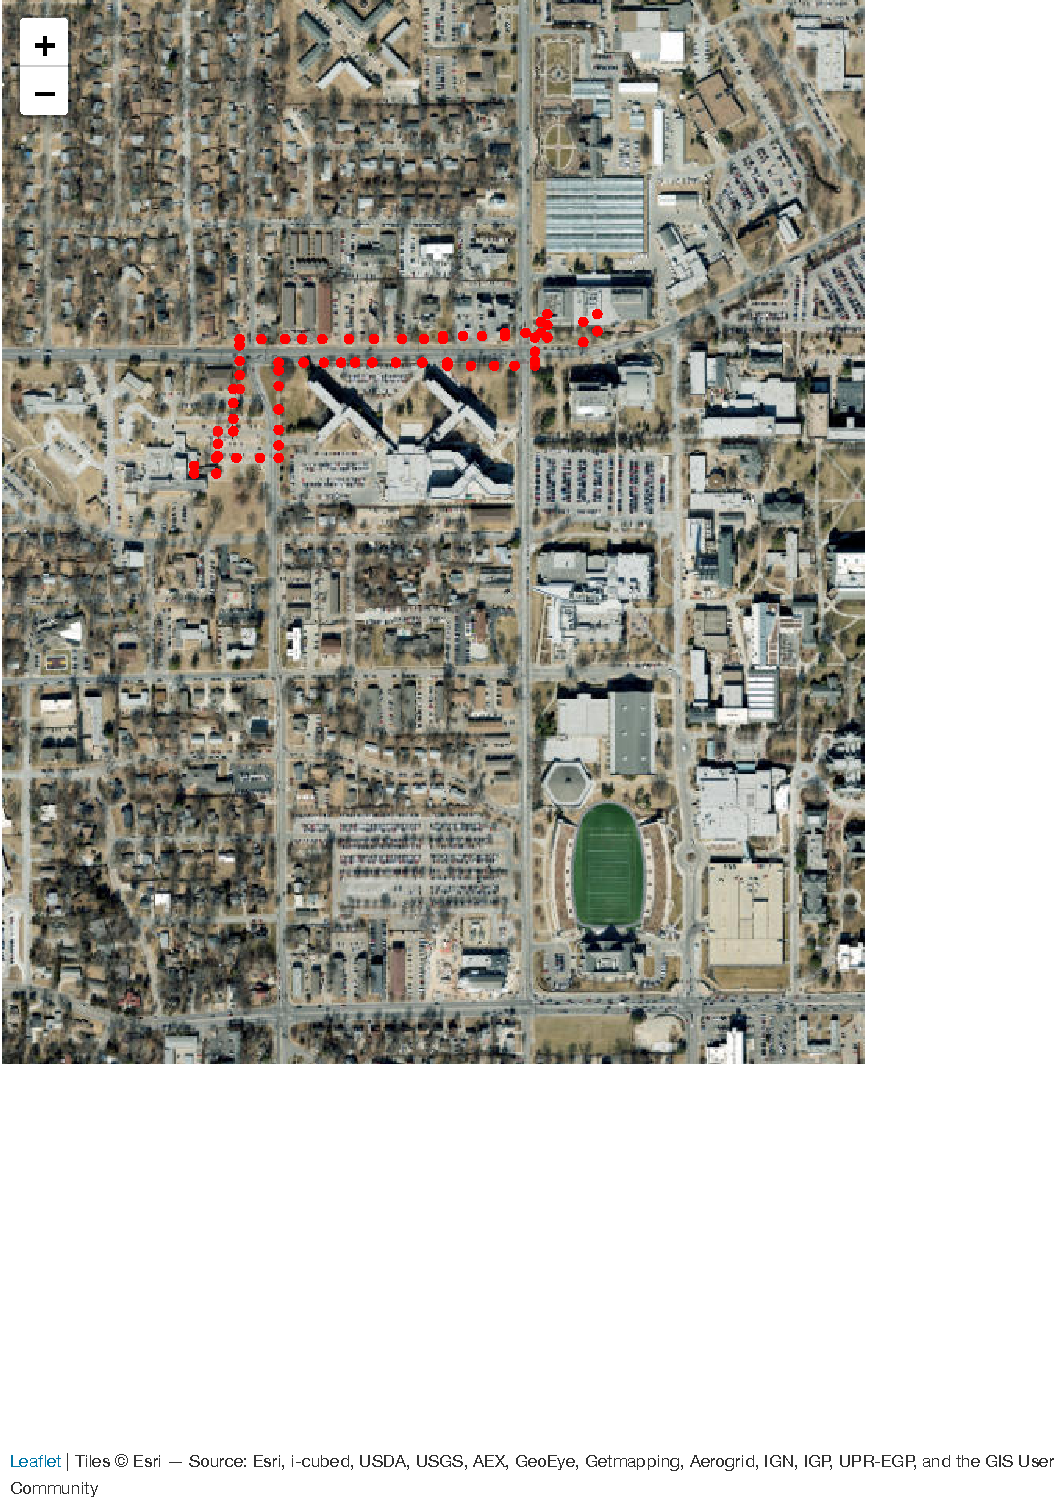
\includegraphics{_main_files/figure-latex/unnamed-chunk-9-1.pdf}

\begin{Shaded}
\begin{Highlighting}[]
\CommentTok{\# Show time series of estimated speed}
\NormalTok{dist.hat }\OtherTok{\textless{}{-}} \FunctionTok{st\_distance}\NormalTok{(df.am\_walk.hat.tree[}\DecValTok{1}\SpecialCharTok{:}\DecValTok{6200}\NormalTok{,],df.am\_walk.hat.tree[}\DecValTok{2}\SpecialCharTok{:}\DecValTok{6201}\NormalTok{,],}\AttributeTok{by\_element=}\ConstantTok{TRUE}\NormalTok{)}
\NormalTok{(}\FunctionTok{sum}\NormalTok{(dist.hat)}\SpecialCharTok{/}\DecValTok{1000}\NormalTok{)}\SpecialCharTok{*}\FloatTok{0.62} \CommentTok{\# Model check. Length of estimated trajectory in miles. Should be \textasciitilde{}26.2}
\end{Highlighting}
\end{Shaded}

\begin{verbatim}
## 0.8350672 [m]
\end{verbatim}

\begin{Shaded}
\begin{Highlighting}[]
\NormalTok{speed.hat }\OtherTok{\textless{}{-}}\NormalTok{ (dist.hat}\SpecialCharTok{/}\FloatTok{0.5}\NormalTok{)}\SpecialCharTok{*}\FloatTok{2.24} \CommentTok{\# units are in miles per hour}
\FunctionTok{plot}\NormalTok{(df.pred}\SpecialCharTok{$}\NormalTok{t[}\SpecialCharTok{{-}}\DecValTok{1}\NormalTok{],speed.hat,}\AttributeTok{xlab=}\StringTok{"Time (seconds)"}\NormalTok{,}\AttributeTok{ylab=}\StringTok{"Velocity (miles per hour)"}\NormalTok{)}
\end{Highlighting}
\end{Shaded}

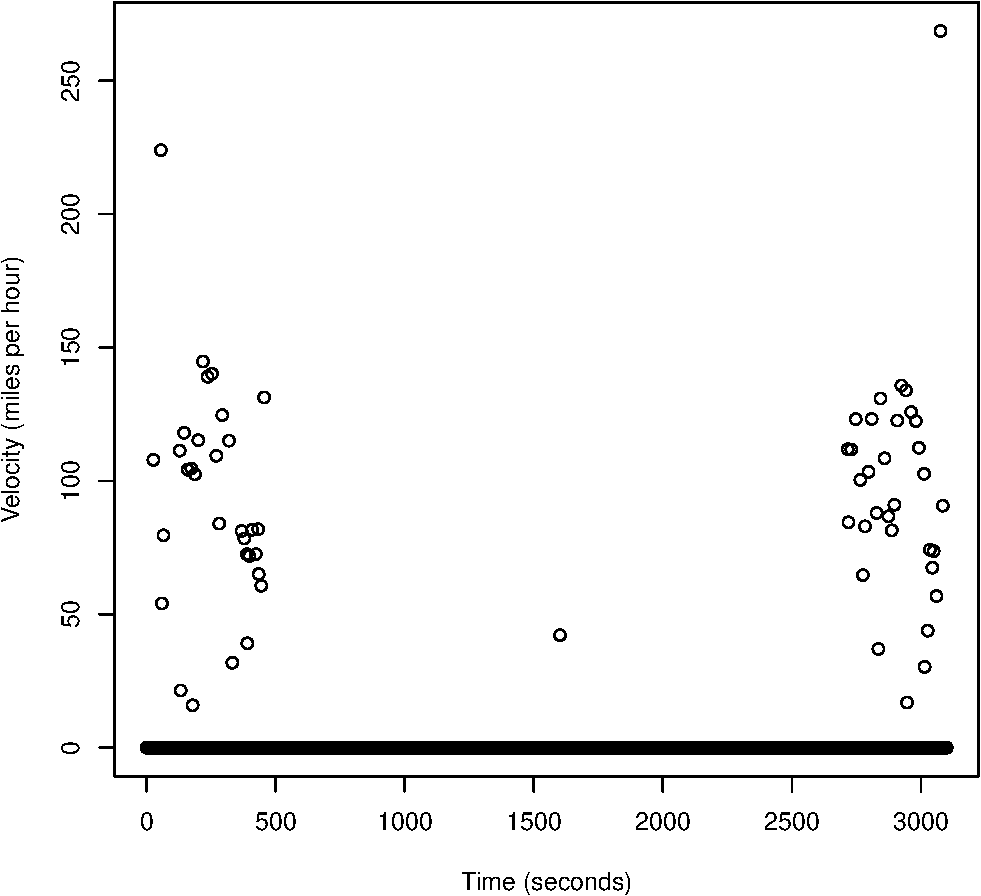
\includegraphics{_main_files/figure-latex/unnamed-chunk-9-2.pdf}

\begin{Shaded}
\begin{Highlighting}[]
\CommentTok{\# Comparison to observed data}
\CommentTok{\# Class discussion about what would happen if we collected more location data?}
\NormalTok{dist }\OtherTok{\textless{}{-}} \FunctionTok{st\_distance}\NormalTok{(am\_walk[}\DecValTok{1}\SpecialCharTok{:}\DecValTok{840}\NormalTok{,],am\_walk[}\DecValTok{2}\SpecialCharTok{:}\DecValTok{841}\NormalTok{,],}\AttributeTok{by\_element=}\ConstantTok{TRUE}\NormalTok{)}
\NormalTok{(}\FunctionTok{sum}\NormalTok{(dist, }\AttributeTok{na.rm =}\NormalTok{ T)}\SpecialCharTok{/}\DecValTok{1000}\NormalTok{)}\SpecialCharTok{*}\FloatTok{0.62}
\end{Highlighting}
\end{Shaded}

\begin{verbatim}
## 0.8918068 [m]
\end{verbatim}

\begin{Shaded}
\begin{Highlighting}[]
\NormalTok{speed }\OtherTok{\textless{}{-}}\NormalTok{ (dist}\SpecialCharTok{/}\FunctionTok{as.numeric}\NormalTok{(}\FunctionTok{diff}\NormalTok{(am\_walk}\SpecialCharTok{$}\NormalTok{time)))}\SpecialCharTok{*}\FloatTok{2.24}
\end{Highlighting}
\end{Shaded}

\begin{verbatim}
## Warning in `/.default`(dist, as.numeric(diff(am_walk$time))): longer object
## length is not a multiple of shorter object length
\end{verbatim}

\hypertarget{visualize-all}{%
\section{Visualize all}\label{visualize-all}}

\begin{Shaded}
\begin{Highlighting}[]
\CommentTok{\# Visualize}
\NormalTok{map\_leaflet }\SpecialCharTok{\%\textgreater{}\%}
  \FunctionTok{addCircleMarkers}\NormalTok{(}\AttributeTok{data =}\NormalTok{ am\_walk, }
                   \AttributeTok{radius =} \DecValTok{3}\NormalTok{, }\AttributeTok{stroke =} \ConstantTok{FALSE}\NormalTok{, }\AttributeTok{fillOpacity =} \FloatTok{0.5}\NormalTok{,}
                   \AttributeTok{color =} \StringTok{"black"}\NormalTok{, }\AttributeTok{label =} \StringTok{"Observed"}\NormalTok{) }\SpecialCharTok{\%\textgreater{}\%} \CommentTok{\# Observed}
  \FunctionTok{addCircleMarkers}\NormalTok{(}\AttributeTok{data =}\NormalTok{ df.am\_walk.hat.lm, }
                   \AttributeTok{radius =} \DecValTok{3}\NormalTok{, }\AttributeTok{stroke =} \ConstantTok{FALSE}\NormalTok{, }\AttributeTok{fillOpacity =} \FloatTok{0.5}\NormalTok{,}
                   \AttributeTok{color =} \StringTok{"red"}\NormalTok{, }\AttributeTok{label =} \StringTok{"Polynomial"}\NormalTok{) }\SpecialCharTok{\%\textgreater{}\%} \CommentTok{\# Polynomial }
  \FunctionTok{addCircleMarkers}\NormalTok{(}\AttributeTok{data =}\NormalTok{ df.am\_walk.hat.gam,}
                   \AttributeTok{radius =} \DecValTok{3}\NormalTok{, }\AttributeTok{stroke =} \ConstantTok{FALSE}\NormalTok{, }\AttributeTok{fillOpacity =} \FloatTok{0.5}\NormalTok{,}
                   \AttributeTok{color =} \StringTok{"green"}\NormalTok{, }\AttributeTok{label =} \StringTok{"GAM"}\NormalTok{) }\SpecialCharTok{\%\textgreater{}\%} \CommentTok{\# GAM}
  \FunctionTok{addCircleMarkers}\NormalTok{(}\AttributeTok{data =}\NormalTok{ df.am\_walk.hat.tree,}
                   \AttributeTok{radius =} \DecValTok{3}\NormalTok{, }\AttributeTok{stroke =} \ConstantTok{FALSE}\NormalTok{, }\AttributeTok{fillOpacity =} \FloatTok{0.5}\NormalTok{,}
                   \AttributeTok{color =} \StringTok{"yellow"}\NormalTok{, }\AttributeTok{label =} \StringTok{"tree"}\NormalTok{) }\CommentTok{\# Regression tree}
\end{Highlighting}
\end{Shaded}

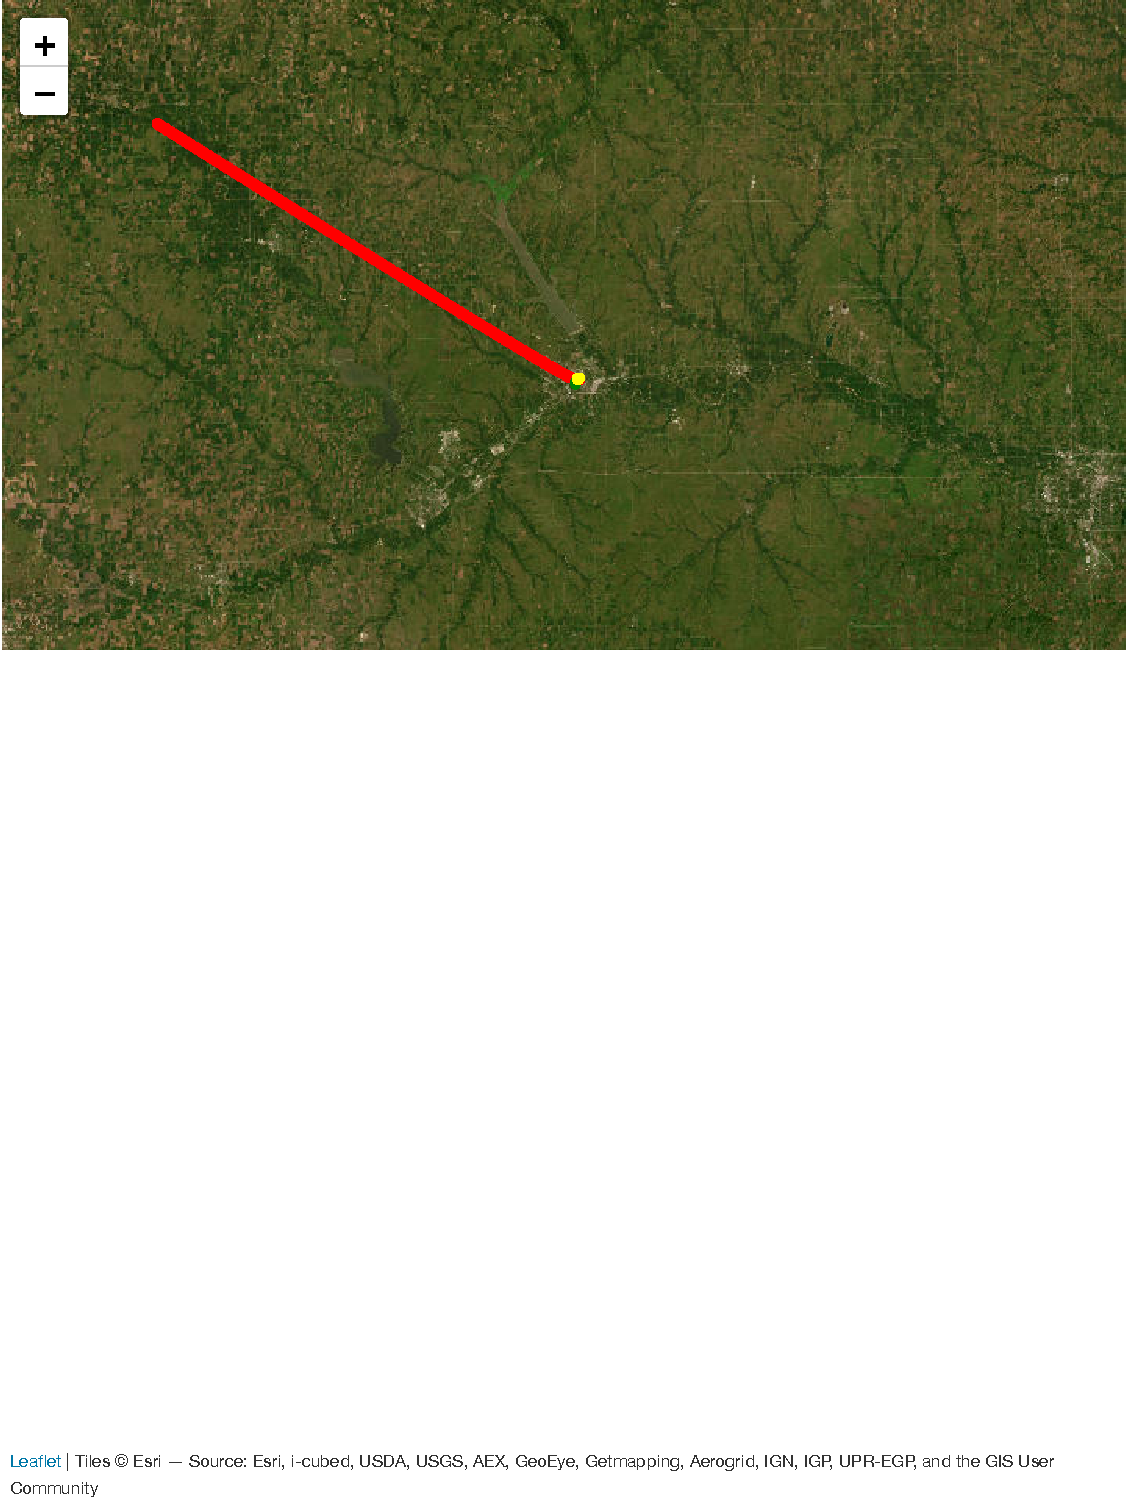
\includegraphics{_main_files/figure-latex/unnamed-chunk-10-1.pdf}
\#\#\# 4. Comments

When I arrived to Laffene I stopped recording and started again from the same point once I was leaving (around 30 min after). The polynomial model is trying to fit a line during the time in between the recordings where there's no data, and went far away from the trajectory. The gam model also tried to estimate the trajectory while there was no recordings and deviated from the real trajectory although not as far away as the polynomial. The regression tree worked really well in following the real trajectory although the way of modeling the data is unrealistic, because it has periods of times with no movement and sudden jumps at high speed.\\
\strut \\
I started and finish the recording inside my office in Throckmorton, so during the time i was inside the building the cellphone was not able to record the location so accurately.

\hypertarget{elevation-data-of-experiment-plot-in-north-agronomy-farm}{%
\chapter{Elevation data of Experiment plot in North Agronomy Farm}\label{elevation-data-of-experiment-plot-in-north-agronomy-farm}}

The goal of this activity is to visualize the elevation data of an experimental site in the North Agronomy Farm at Kansas State University. Also my goal is to predict elevation with different models and infer at what location we observe the lowest and highest elevation point.

\hypertarget{librarires}{%
\section{Librarires}\label{librarires}}

\begin{Shaded}
\begin{Highlighting}[]
\FunctionTok{library}\NormalTok{(sf)}
\FunctionTok{library}\NormalTok{(sp)}
\FunctionTok{library}\NormalTok{(raster)}
\FunctionTok{library}\NormalTok{(tidyverse)}
\end{Highlighting}
\end{Shaded}

\hypertarget{kansas-boundary}{%
\section{Kansas boundary}\label{kansas-boundary}}

\begin{Shaded}
\begin{Highlighting}[]
\CommentTok{\# Download shapefile of Kansas from census.gov}
\FunctionTok{download.file}\NormalTok{(}\StringTok{"http://www2.census.gov/geo/tiger/GENZ2015/shp/cb\_2015\_us\_state\_20m.zip"}\NormalTok{, }\AttributeTok{destfile =} \StringTok{"states.zip"}\NormalTok{)}
\FunctionTok{unzip}\NormalTok{(}\StringTok{"states.zip"}\NormalTok{)}
\NormalTok{sf.us }\OtherTok{\textless{}{-}} \FunctionTok{st\_read}\NormalTok{(}\StringTok{"cb\_2015\_us\_state\_20m.shp"}\NormalTok{)}
\end{Highlighting}
\end{Shaded}

\begin{verbatim}
## Reading layer `cb_2015_us_state_20m' from data source 
##   `/Users/mariavalentinapereyrapicabea/Desktop/Maestria/Spring 2024/STAT 764/R STAT 764/bookdown/cb_2015_us_state_20m.shp' 
##   using driver `ESRI Shapefile'
## Simple feature collection with 52 features and 9 fields
## Geometry type: MULTIPOLYGON
## Dimension:     XY
## Bounding box:  xmin: -179.1743 ymin: 17.91377 xmax: 179.7739 ymax: 71.35256
## Geodetic CRS:  NAD83
\end{verbatim}

\begin{Shaded}
\begin{Highlighting}[]
\NormalTok{sf.kansas }\OtherTok{\textless{}{-}}\NormalTok{ sf.us[}\DecValTok{48}\NormalTok{,}\DecValTok{6}\NormalTok{]}
\NormalTok{sf.kansas }\OtherTok{\textless{}{-}} \FunctionTok{as}\NormalTok{(sf.kansas, }\StringTok{\textquotesingle{}Spatial\textquotesingle{}}\NormalTok{)}
\FunctionTok{plot}\NormalTok{(sf.kansas,}\AttributeTok{main=}\StringTok{""}\NormalTok{,}\AttributeTok{col=}\StringTok{"white"}\NormalTok{)}
\end{Highlighting}
\end{Shaded}


\includegraphics{_main_files/figure-latex/unnamed-chunk-12-1.pdf}

\hypertarget{my-data-north-agronomy-farm}{%
\section{My data: North Agronomy Farm}\label{my-data-north-agronomy-farm}}

\begin{Shaded}
\begin{Highlighting}[]
\CommentTok{\# Make shapefile of study area around Manhattan KS}
\NormalTok{url }\OtherTok{\textless{}{-}} \StringTok{"https://www.dropbox.com/scl/fi/b7d9254b8f26mhu6pc2km/Experiment\_walk.gpx?rlkey=nmph96rzfz8rxmwxsxg3wn4p1\&dl=1"}
\NormalTok{pt.study.area }\OtherTok{\textless{}{-}} \FunctionTok{st\_read}\NormalTok{(}\AttributeTok{dsn=}\NormalTok{url,}\AttributeTok{layer=}\StringTok{"track\_points"}\NormalTok{)}
\end{Highlighting}
\end{Shaded}

\begin{verbatim}
## Reading layer `track_points' from data source 
##   `https://www.dropbox.com/scl/fi/b7d9254b8f26mhu6pc2km/Experiment_walk.gpx?rlkey=nmph96rzfz8rxmwxsxg3wn4p1&dl=1' 
##   using driver `GPX'
## Simple feature collection with 318 features and 26 fields
## Geometry type: POINT
## Dimension:     XY
## Bounding box:  xmin: -96.59412 ymin: 39.20585 xmax: -96.5938 ymax: 39.2064
## Geodetic CRS:  WGS 84
\end{verbatim}

\begin{Shaded}
\begin{Highlighting}[]
\NormalTok{sf.study.area  }\OtherTok{\textless{}{-}} \FunctionTok{st\_polygon}\NormalTok{(}\FunctionTok{list}\NormalTok{(}\FunctionTok{rbind}\NormalTok{(}\FunctionTok{st\_coordinates}\NormalTok{(pt.study.area),}\FunctionTok{st\_coordinates}\NormalTok{(pt.study.area)[}\DecValTok{1}\NormalTok{,])))}
\NormalTok{sf.study.area }\OtherTok{\textless{}{-}} \FunctionTok{st\_buffer}\NormalTok{(sf.study.area, .}\DecValTok{00006}\NormalTok{)}
\NormalTok{sf.study.area }\OtherTok{\textless{}{-}} \FunctionTok{st\_sf}\NormalTok{(}\FunctionTok{st\_sfc}\NormalTok{(sf.study.area), }\AttributeTok{crs =} \FunctionTok{crs}\NormalTok{(sf.kansas))}

\CommentTok{\# Kansas + North farm data}
\NormalTok{\{}\FunctionTok{plot}\NormalTok{(sf.kansas,}\AttributeTok{main=}\StringTok{""}\NormalTok{,}\AttributeTok{col=}\StringTok{"white"}\NormalTok{,}\AttributeTok{xlim=}\FunctionTok{c}\NormalTok{(}\SpecialCharTok{{-}}\FloatTok{102.0517}\NormalTok{,}\SpecialCharTok{{-}}\FloatTok{94.59193}\NormalTok{),}\AttributeTok{ylim=}\FunctionTok{c}\NormalTok{(}\FloatTok{36.99308}\NormalTok{,}\FloatTok{40.00308}\NormalTok{))}
\FunctionTok{plot}\NormalTok{(sf.study.area, }\AttributeTok{add=}\ConstantTok{TRUE}\NormalTok{, }\AttributeTok{col=}\StringTok{"red"}\NormalTok{)\}}
\end{Highlighting}
\end{Shaded}


\includegraphics{_main_files/figure-latex/unnamed-chunk-13-1.pdf}

\hypertarget{extract-elevation}{%
\section{Extract elevation}\label{extract-elevation}}

\begin{Shaded}
\begin{Highlighting}[]
\NormalTok{url }\OtherTok{\textless{}{-}} \StringTok{"https://www.dropbox.com/scl/fi/b7d9254b8f26mhu6pc2km/Experiment\_walk.gpx?rlkey=nmph96rzfz8rxmwxsxg3wn4p1\&dl=1"}

\NormalTok{pt.elev }\OtherTok{\textless{}{-}} \FunctionTok{st\_read}\NormalTok{(}\AttributeTok{dsn=}\NormalTok{url,}\AttributeTok{layer=}\StringTok{"track\_points"}\NormalTok{)}
\end{Highlighting}
\end{Shaded}

\begin{verbatim}
## Reading layer `track_points' from data source 
##   `https://www.dropbox.com/scl/fi/b7d9254b8f26mhu6pc2km/Experiment_walk.gpx?rlkey=nmph96rzfz8rxmwxsxg3wn4p1&dl=1' 
##   using driver `GPX'
## Simple feature collection with 318 features and 26 fields
## Geometry type: POINT
## Dimension:     XY
## Bounding box:  xmin: -96.59412 ymin: 39.20585 xmax: -96.5938 ymax: 39.2064
## Geodetic CRS:  WGS 84
\end{verbatim}

\begin{Shaded}
\begin{Highlighting}[]
\NormalTok{pt.elev }\OtherTok{\textless{}{-}}\NormalTok{ pt.elev[,}\DecValTok{4}\NormalTok{] }\CommentTok{\# Keep only elevation}
\NormalTok{pt.elev }\OtherTok{\textless{}{-}}\NormalTok{ pt.elev[}\SpecialCharTok{{-}}\FunctionTok{c}\NormalTok{(}\DecValTok{1}\SpecialCharTok{:}\DecValTok{15}\NormalTok{),]}
\CommentTok{\#pt.elev \textless{}{-} rbind(pt.elev,pt.study.area[,4])}
\end{Highlighting}
\end{Shaded}

\hypertarget{visualize-boundary-elevation}{%
\section{Visualize boundary + elevation}\label{visualize-boundary-elevation}}

\begin{Shaded}
\begin{Highlighting}[]
\NormalTok{\{}\FunctionTok{plot}\NormalTok{(sf.study.area)}
\FunctionTok{plot}\NormalTok{(pt.elev,}\AttributeTok{add=}\ConstantTok{TRUE}\NormalTok{)\}}
\end{Highlighting}
\end{Shaded}

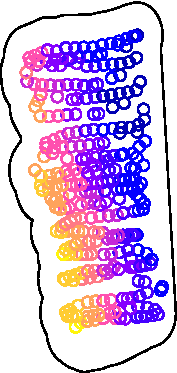
\includegraphics{_main_files/figure-latex/unnamed-chunk-15-1.pdf}

\begin{Shaded}
\begin{Highlighting}[]
\FunctionTok{hist}\NormalTok{(pt.elev}\SpecialCharTok{$}\NormalTok{ele,}\AttributeTok{col=}\StringTok{"grey"}\NormalTok{)}
\end{Highlighting}
\end{Shaded}

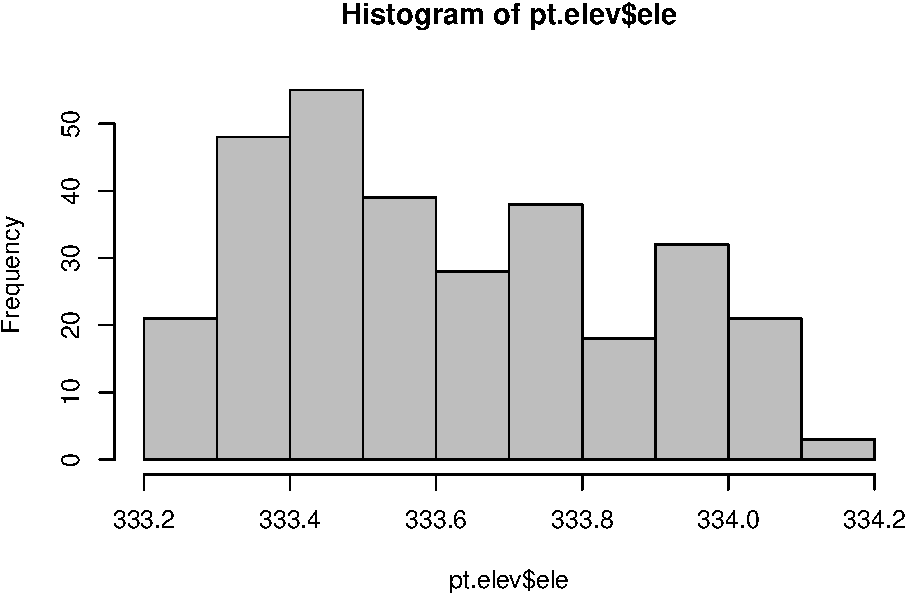
\includegraphics{_main_files/figure-latex/unnamed-chunk-15-2.pdf}

\begin{Shaded}
\begin{Highlighting}[]
\FunctionTok{summary}\NormalTok{(pt.elev}\SpecialCharTok{$}\NormalTok{ele)}
\end{Highlighting}
\end{Shaded}

\begin{verbatim}
##    Min. 1st Qu.  Median    Mean 3rd Qu.    Max. 
##   333.2   333.5   333.6   333.7   333.8   334.2
\end{verbatim}

\begin{Shaded}
\begin{Highlighting}[]
\FunctionTok{ggplot}\NormalTok{() }\SpecialCharTok{+}
  \FunctionTok{geom\_sf}\NormalTok{(}\AttributeTok{data=}\NormalTok{sf.study.area) }\SpecialCharTok{+}
  \FunctionTok{labs}\NormalTok{(}\AttributeTok{subtitle =} \StringTok{"North Agronomy Farm"}\NormalTok{)}\SpecialCharTok{+}
  \FunctionTok{geom\_sf}\NormalTok{(}\AttributeTok{data=}\NormalTok{pt.elev, }\FunctionTok{aes}\NormalTok{(}\AttributeTok{color =}\NormalTok{ ele), }\AttributeTok{size =} \DecValTok{2}\NormalTok{)}\SpecialCharTok{+}
  \FunctionTok{scale\_color\_gradient}\NormalTok{(}\AttributeTok{low=}\StringTok{"blue"}\NormalTok{, }\AttributeTok{high=}\StringTok{"red"}\NormalTok{, }\AttributeTok{name =} \StringTok{"Elevation (m)"}\NormalTok{)}\SpecialCharTok{+}
  \FunctionTok{theme}\NormalTok{(}\AttributeTok{panel.background =} \FunctionTok{element\_blank}\NormalTok{(),}
        \AttributeTok{axis.text =} \FunctionTok{element\_blank}\NormalTok{())}
\end{Highlighting}
\end{Shaded}

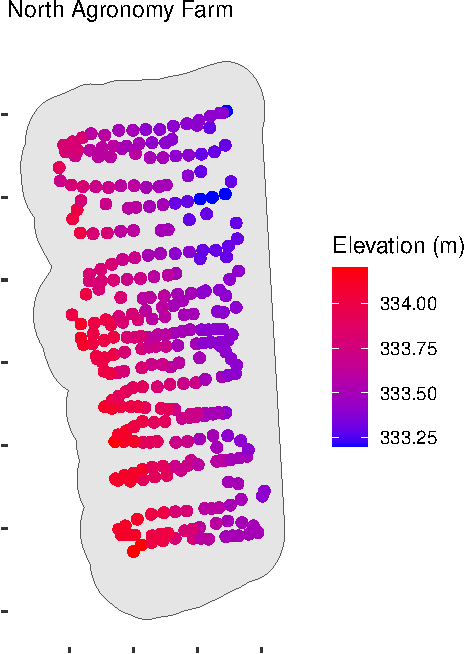
\includegraphics{_main_files/figure-latex/unnamed-chunk-15-3.pdf}

\begin{Shaded}
\begin{Highlighting}[]
\CommentTok{\# Visualize with satelite image }
\NormalTok{mapview}\SpecialCharTok{::}\FunctionTok{mapview}\NormalTok{(sf.study.area)  }
\end{Highlighting}
\end{Shaded}

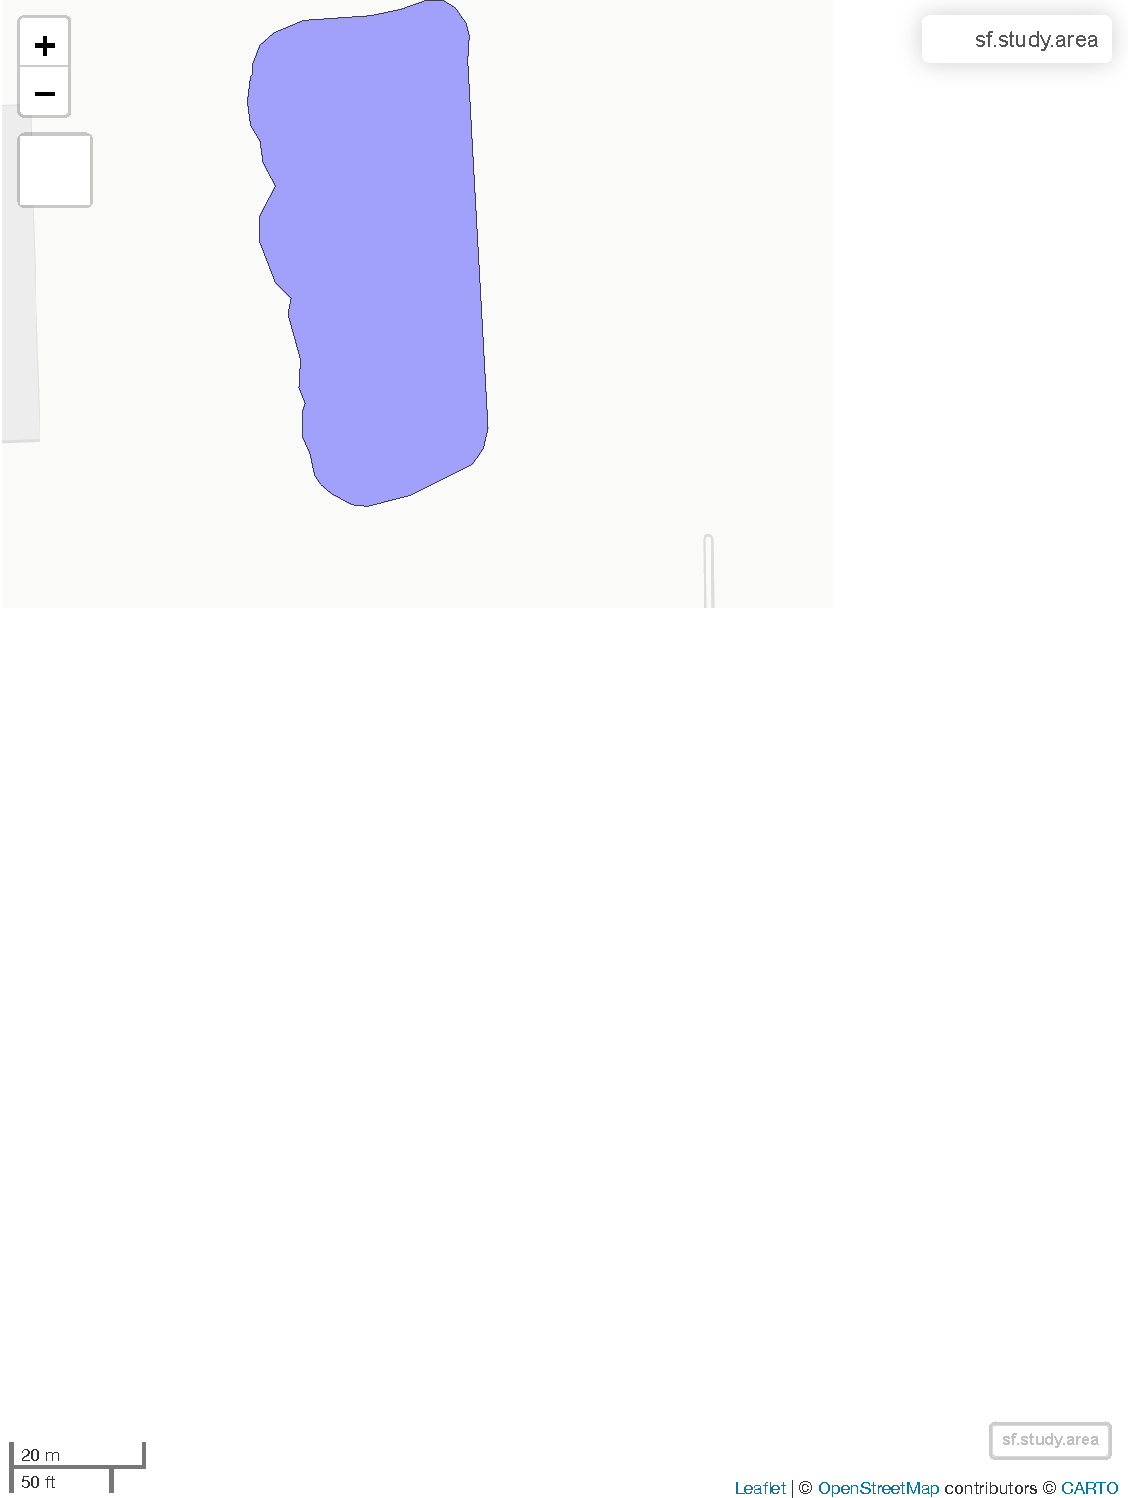
\includegraphics{_main_files/figure-latex/unnamed-chunk-15-4.pdf}

\begin{Shaded}
\begin{Highlighting}[]
\CommentTok{\# Transform pointfiles and shapefiles to utm zone to a planar coordinate reference system}
\NormalTok{pt.elev.utm }\OtherTok{\textless{}{-}} \FunctionTok{st\_transform}\NormalTok{(pt.elev,}\FunctionTok{CRS}\NormalTok{(}\StringTok{"+proj=utm +zone=14 +datum=WGS84  +units=m"}\NormalTok{))}
\NormalTok{sf.study.area.utm }\OtherTok{\textless{}{-}} \FunctionTok{st\_transform}\NormalTok{(sf.study.area,}\FunctionTok{CRS}\NormalTok{(}\StringTok{"+proj=utm +zone=14 +datum=WGS84  +units=m"}\NormalTok{))}
\end{Highlighting}
\end{Shaded}

\begin{Shaded}
\begin{Highlighting}[]
\CommentTok{\# Make data.frame for statistical analysis}
\NormalTok{df.elev }\OtherTok{\textless{}{-}} \FunctionTok{data.frame}\NormalTok{ (}\AttributeTok{elev =}\NormalTok{ pt.elev}\SpecialCharTok{$}\NormalTok{ele,}
                       \AttributeTok{long =} \FunctionTok{st\_coordinates}\NormalTok{(pt.elev)[,}\DecValTok{1}\NormalTok{],}
                       \AttributeTok{lat =} \FunctionTok{st\_coordinates}\NormalTok{(pt.elev)[,}\DecValTok{2}\NormalTok{],}
                       \AttributeTok{s1 =} \FunctionTok{st\_coordinates}\NormalTok{(pt.elev.utm)[,}\DecValTok{1}\NormalTok{],}
                       \AttributeTok{s2 =} \FunctionTok{st\_coordinates}\NormalTok{(pt.elev.utm)[,}\DecValTok{2}\NormalTok{])}
\end{Highlighting}
\end{Shaded}

\hypertarget{models}{%
\section{Models}\label{models}}

\hypertarget{linear-with-iid-errors}{%
\subsection{1. Linear with iid errors}\label{linear-with-iid-errors}}

\begin{Shaded}
\begin{Highlighting}[]
\CommentTok{\# Statistical analysis 1: non{-}hierarchical linear model with iid errors}
\NormalTok{m1 }\OtherTok{\textless{}{-}} \FunctionTok{lm}\NormalTok{(elev}\SpecialCharTok{\textasciitilde{}}\NormalTok{s1}\SpecialCharTok{+}\FunctionTok{I}\NormalTok{(s1}\SpecialCharTok{\^{}}\DecValTok{2}\NormalTok{)}\SpecialCharTok{+}\NormalTok{s2}\SpecialCharTok{+}\FunctionTok{I}\NormalTok{(s2}\SpecialCharTok{\^{}}\DecValTok{2}\NormalTok{),}\AttributeTok{data=}\NormalTok{df.elev)}
\CommentTok{\# Make raster of study area to be able to map predictions from m1}
\NormalTok{rl.E.y\_lin }\OtherTok{\textless{}{-}} \FunctionTok{raster}\NormalTok{(,}\AttributeTok{nrow=}\DecValTok{100}\NormalTok{,}\AttributeTok{ncols=}\DecValTok{100}\NormalTok{,}\AttributeTok{ext=}\FunctionTok{extent}\NormalTok{(sf.study.area.utm),}\AttributeTok{crs=}\FunctionTok{crs}\NormalTok{(sf.study.area.utm))}
\CommentTok{\# Make data.frame to be able to make predictions at each pixel (cell of raster)}
\NormalTok{df.pred }\OtherTok{\textless{}{-}} \FunctionTok{data.frame}\NormalTok{(}\AttributeTok{elev =} \ConstantTok{NA}\NormalTok{,}
                      \AttributeTok{s1 =} \FunctionTok{xyFromCell}\NormalTok{(rl.E.y\_lin,}\AttributeTok{cell=}\DecValTok{1}\SpecialCharTok{:}\FunctionTok{length}\NormalTok{(rl.E.y\_lin[]))[,}\DecValTok{1}\NormalTok{],}
                      \AttributeTok{s2 =} \FunctionTok{xyFromCell}\NormalTok{(rl.E.y\_lin,}\AttributeTok{cell=}\DecValTok{1}\SpecialCharTok{:}\FunctionTok{length}\NormalTok{(rl.E.y\_lin[]))[,}\DecValTok{2}\NormalTok{])}

\CommentTok{\# Make spatial predictions at each pixel}
\NormalTok{df.pred}\SpecialCharTok{$}\NormalTok{elev }\OtherTok{\textless{}{-}} \FunctionTok{predict}\NormalTok{(m1,df.pred[,}\DecValTok{2}\SpecialCharTok{:}\DecValTok{3}\NormalTok{])}

\CommentTok{\# View first 6 rows of predictions}
\FunctionTok{head}\NormalTok{(df.pred) }
\end{Highlighting}
\end{Shaded}

\begin{verbatim}
##       elev       s1      s2
## 1 333.9162 707730.7 4342447
## 2 333.9042 707731.1 4342447
## 3 333.8923 707731.4 4342447
## 4 333.8803 707731.8 4342447
## 5 333.8684 707732.2 4342447
## 6 333.8564 707732.5 4342447
\end{verbatim}

\begin{Shaded}
\begin{Highlighting}[]
\CommentTok{\# Fill raster file with predictions }
\NormalTok{rl.E.y\_lin[] }\OtherTok{\textless{}{-}} \FunctionTok{c}\NormalTok{(df.pred}\SpecialCharTok{$}\NormalTok{elev)}

\NormalTok{rl.E.y\_lin }\OtherTok{\textless{}{-}} \FunctionTok{mask}\NormalTok{(rl.E.y\_lin,sf.study.area.utm)}

\CommentTok{\# Estimate coordinates and amount of maximum elevation}
\FunctionTok{xyFromCell}\NormalTok{(rl.E.y\_lin,}\AttributeTok{cell=}\FunctionTok{which.max}\NormalTok{(rl.E.y\_lin[]))}
\end{Highlighting}
\end{Shaded}

\begin{verbatim}
##             x       y
## [1,] 707740.3 4342381
\end{verbatim}

\begin{Shaded}
\begin{Highlighting}[]
\NormalTok{rl.E.y\_lin[}\FunctionTok{which.max}\NormalTok{(rl.E.y\_lin[])]}
\end{Highlighting}
\end{Shaded}

\begin{verbatim}
## [1] 334.2931
\end{verbatim}

\begin{Shaded}
\begin{Highlighting}[]
\CommentTok{\# Plot estimate coordinates of maximum elevation}
\NormalTok{\{}\FunctionTok{plot}\NormalTok{(rl.E.y\_lin, }\AttributeTok{main =} \StringTok{"Linear with iid errors"}\NormalTok{) }\CommentTok{\# Plot map of predictions}
\FunctionTok{plot}\NormalTok{(sf.study.area.utm,}\AttributeTok{add=}\ConstantTok{TRUE}\NormalTok{)}
\FunctionTok{points}\NormalTok{(}\FunctionTok{xyFromCell}\NormalTok{(rl.E.y\_lin,}\AttributeTok{cell=}\FunctionTok{which.max}\NormalTok{(rl.E.y\_lin[])),}\AttributeTok{col=}\StringTok{"purple"}\NormalTok{,}\AttributeTok{pch=}\StringTok{"*"}\NormalTok{,}\AttributeTok{cex=}\DecValTok{3}\NormalTok{)}
\FunctionTok{points}\NormalTok{(}\FunctionTok{xyFromCell}\NormalTok{(rl.E.y\_lin,}\AttributeTok{cell=}\FunctionTok{which.min}\NormalTok{(rl.E.y\_lin[])),}\AttributeTok{col=}\StringTok{"blue"}\NormalTok{,}\AttributeTok{pch=}\StringTok{"*"}\NormalTok{,}\AttributeTok{cex=}\DecValTok{3}\NormalTok{)\}}
\end{Highlighting}
\end{Shaded}

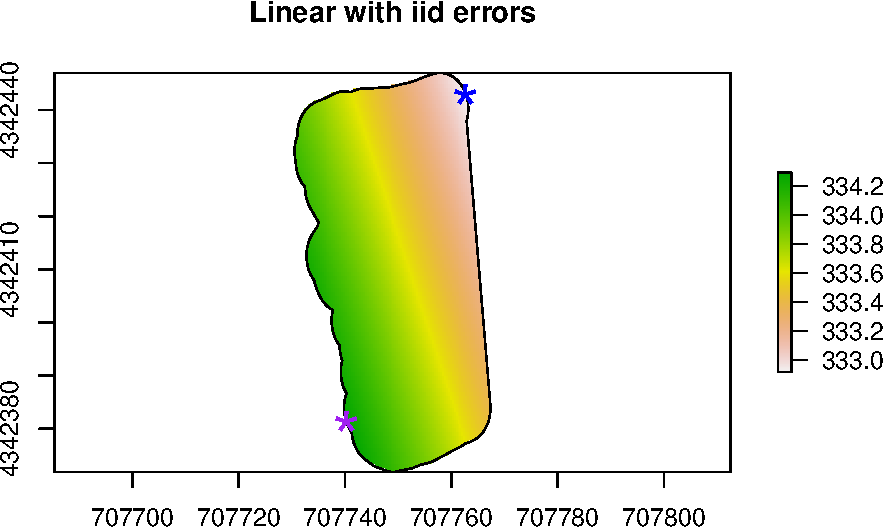
\includegraphics{_main_files/figure-latex/unnamed-chunk-18-1.pdf}

\hypertarget{gam}{%
\subsection{2. GAM}\label{gam}}

\begin{Shaded}
\begin{Highlighting}[]
\CommentTok{\# Try low{-}rank Gaussian process (i.e., modern kriging model)}
\FunctionTok{library}\NormalTok{(mgcv)}
\NormalTok{m1 }\OtherTok{\textless{}{-}} \FunctionTok{gam}\NormalTok{(elev}\SpecialCharTok{\textasciitilde{}}\FunctionTok{s}\NormalTok{(s1,s2,}\AttributeTok{bs=}\StringTok{"gp"}\NormalTok{),}\AttributeTok{data=}\NormalTok{df.elev)}

\CommentTok{\# Make raster of study area to be able to map predictions from m1}
\NormalTok{rl.E.y\_gam }\OtherTok{\textless{}{-}} \FunctionTok{raster}\NormalTok{(,}\AttributeTok{nrow=}\DecValTok{100}\NormalTok{,}\AttributeTok{ncols=}\DecValTok{100}\NormalTok{,}\AttributeTok{ext=}\FunctionTok{extent}\NormalTok{(sf.study.area.utm),}\AttributeTok{crs=}\FunctionTok{crs}\NormalTok{(sf.study.area.utm))}
\CommentTok{\# Make data.frame to be able to make predictions at each pixel (cell of raster)}
\NormalTok{df.pred }\OtherTok{\textless{}{-}} \FunctionTok{data.frame}\NormalTok{(}\AttributeTok{elev =} \ConstantTok{NA}\NormalTok{,}
                      \AttributeTok{s1 =} \FunctionTok{xyFromCell}\NormalTok{(rl.E.y\_gam,}\AttributeTok{cell=}\DecValTok{1}\SpecialCharTok{:}\FunctionTok{length}\NormalTok{(rl.E.y\_gam[]))[,}\DecValTok{1}\NormalTok{],}
                      \AttributeTok{s2 =} \FunctionTok{xyFromCell}\NormalTok{(rl.E.y\_gam,}\AttributeTok{cell=}\DecValTok{1}\SpecialCharTok{:}\FunctionTok{length}\NormalTok{(rl.E.y\_gam[]))[,}\DecValTok{2}\NormalTok{])}

\CommentTok{\# Make spatial predictions at each pixel}
\NormalTok{df.pred}\SpecialCharTok{$}\NormalTok{elev }\OtherTok{\textless{}{-}} \FunctionTok{predict}\NormalTok{(m1,df.pred[,}\DecValTok{2}\SpecialCharTok{:}\DecValTok{3}\NormalTok{])}

\CommentTok{\# View first 6 rows of predictions}
\FunctionTok{head}\NormalTok{(df.pred) }
\end{Highlighting}
\end{Shaded}

\begin{verbatim}
##       elev       s1      s2
## 1 333.8337 707730.7 4342447
## 2 333.8222 707731.1 4342447
## 3 333.8107 707731.4 4342447
## 4 333.7993 707731.8 4342447
## 5 333.7879 707732.2 4342447
## 6 333.7766 707732.5 4342447
\end{verbatim}

\begin{Shaded}
\begin{Highlighting}[]
\CommentTok{\# Fill raster file with predictions }
\NormalTok{rl.E.y\_gam[] }\OtherTok{\textless{}{-}} \FunctionTok{c}\NormalTok{(df.pred}\SpecialCharTok{$}\NormalTok{elev)}

\NormalTok{rl.E.y\_gam }\OtherTok{\textless{}{-}} \FunctionTok{mask}\NormalTok{(rl.E.y\_gam,sf.study.area.utm)}

\CommentTok{\# Estimate coordinates and amount of maximum elevation}
\FunctionTok{xyFromCell}\NormalTok{(rl.E.y\_gam,}\AttributeTok{cell=}\FunctionTok{which.max}\NormalTok{(rl.E.y\_gam[]))}
\end{Highlighting}
\end{Shaded}

\begin{verbatim}
##             x       y
## [1,] 707740.3 4342381
\end{verbatim}

\begin{Shaded}
\begin{Highlighting}[]
\NormalTok{rl.E.y\_gam[}\FunctionTok{which.max}\NormalTok{(rl.E.y\_gam[])]}
\end{Highlighting}
\end{Shaded}

\begin{verbatim}
## [1] 334.3422
\end{verbatim}

\begin{Shaded}
\begin{Highlighting}[]
\CommentTok{\# Plot estimate coordinates of maximum elevation}
\NormalTok{\{}\FunctionTok{plot}\NormalTok{(rl.E.y\_gam, }\AttributeTok{main =} \StringTok{"Generalized additive model"}\NormalTok{) }\CommentTok{\# Plot map of predictions}
\FunctionTok{plot}\NormalTok{(sf.study.area.utm,}\AttributeTok{add=}\ConstantTok{TRUE}\NormalTok{)}
\FunctionTok{points}\NormalTok{(}\FunctionTok{xyFromCell}\NormalTok{(rl.E.y\_gam,}\AttributeTok{cell=}\FunctionTok{which.max}\NormalTok{(rl.E.y\_gam[])),}\AttributeTok{col=}\StringTok{"purple"}\NormalTok{,}\AttributeTok{pch=}\StringTok{"*"}\NormalTok{,}\AttributeTok{cex=}\DecValTok{3}\NormalTok{)}
\FunctionTok{points}\NormalTok{(}\FunctionTok{xyFromCell}\NormalTok{(rl.E.y\_lin,}\AttributeTok{cell=}\FunctionTok{which.min}\NormalTok{(rl.E.y\_lin[])),}\AttributeTok{col=}\StringTok{"blue"}\NormalTok{,}\AttributeTok{pch=}\StringTok{"*"}\NormalTok{,}\AttributeTok{cex=}\DecValTok{3}\NormalTok{)\}}
\end{Highlighting}
\end{Shaded}

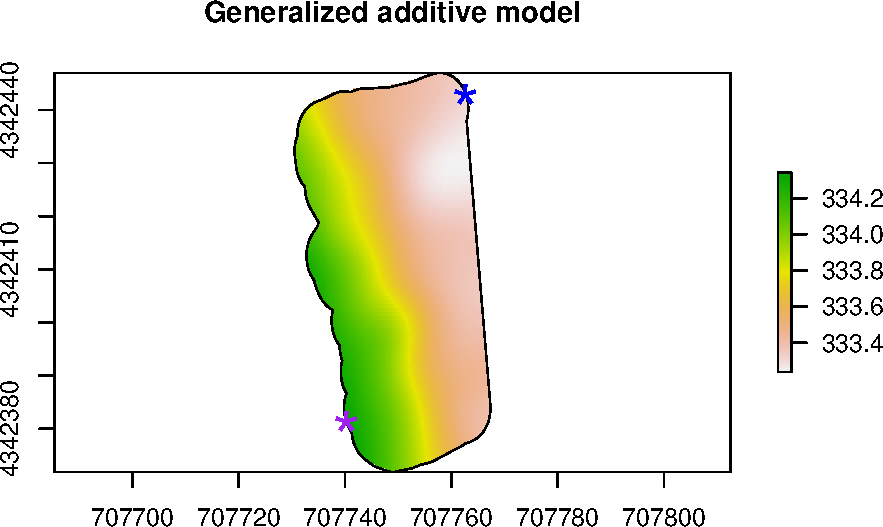
\includegraphics{_main_files/figure-latex/unnamed-chunk-19-1.pdf}

\hypertarget{regression-tree-1}{%
\subsection{3. Regression tree}\label{regression-tree-1}}

\begin{Shaded}
\begin{Highlighting}[]
\CommentTok{\# Try a regression tree instead!}
\FunctionTok{library}\NormalTok{(rpart)}
\NormalTok{m1 }\OtherTok{\textless{}{-}} \FunctionTok{rpart}\NormalTok{(elev}\SpecialCharTok{\textasciitilde{}}\NormalTok{s1}\SpecialCharTok{+}\NormalTok{s2,}\AttributeTok{data=}\NormalTok{df.elev)}

\CommentTok{\# Make raster of study area to be able to map predictions from m1}
\NormalTok{rl.E.y\_rt }\OtherTok{\textless{}{-}} \FunctionTok{raster}\NormalTok{(,}\AttributeTok{nrow=}\DecValTok{100}\NormalTok{,}\AttributeTok{ncols=}\DecValTok{100}\NormalTok{,}\AttributeTok{ext=}\FunctionTok{extent}\NormalTok{(sf.study.area.utm),}\AttributeTok{crs=}\FunctionTok{crs}\NormalTok{(sf.study.area.utm))}
\CommentTok{\# Make data.frame to be able to make predictions at each pixel (cell of raster)}
\NormalTok{df.pred }\OtherTok{\textless{}{-}} \FunctionTok{data.frame}\NormalTok{(}\AttributeTok{elev =} \ConstantTok{NA}\NormalTok{,}
                      \AttributeTok{s1 =} \FunctionTok{xyFromCell}\NormalTok{(rl.E.y\_rt,}\AttributeTok{cell=}\DecValTok{1}\SpecialCharTok{:}\FunctionTok{length}\NormalTok{(rl.E.y\_rt[]))[,}\DecValTok{1}\NormalTok{],}
                      \AttributeTok{s2 =} \FunctionTok{xyFromCell}\NormalTok{(rl.E.y\_rt,}\AttributeTok{cell=}\DecValTok{1}\SpecialCharTok{:}\FunctionTok{length}\NormalTok{(rl.E.y\_rt[]))[,}\DecValTok{2}\NormalTok{])}

\CommentTok{\# Make spatial predictions at each pixel}
\NormalTok{df.pred}\SpecialCharTok{$}\NormalTok{elev }\OtherTok{\textless{}{-}} \FunctionTok{predict}\NormalTok{(m1,df.pred[,}\DecValTok{2}\SpecialCharTok{:}\DecValTok{3}\NormalTok{])}

\CommentTok{\# View first 6 rows of predictions}
\FunctionTok{head}\NormalTok{(df.pred) }
\end{Highlighting}
\end{Shaded}

\begin{verbatim}
##       elev       s1      s2
## 1 333.7143 707730.7 4342447
## 2 333.7143 707731.1 4342447
## 3 333.7143 707731.4 4342447
## 4 333.7143 707731.8 4342447
## 5 333.7143 707732.2 4342447
## 6 333.7143 707732.5 4342447
\end{verbatim}

\begin{Shaded}
\begin{Highlighting}[]
\CommentTok{\# Fill raster file with predictions }
\NormalTok{rl.E.y\_rt[] }\OtherTok{\textless{}{-}} \FunctionTok{c}\NormalTok{(df.pred}\SpecialCharTok{$}\NormalTok{elev)}

\NormalTok{rl.E.y\_rt }\OtherTok{\textless{}{-}} \FunctionTok{mask}\NormalTok{(rl.E.y\_rt,sf.study.area.utm)}

\CommentTok{\# Estimate coordinates and amount of maximum elevation}
\FunctionTok{xyFromCell}\NormalTok{(rl.E.y\_rt,}\AttributeTok{cell=}\FunctionTok{which.max}\NormalTok{(rl.E.y\_rt[]))}
\end{Highlighting}
\end{Shaded}

\begin{verbatim}
##             x       y
## [1,] 707737.7 4342400
\end{verbatim}

\begin{Shaded}
\begin{Highlighting}[]
\NormalTok{rl.E.y\_rt[}\FunctionTok{which.max}\NormalTok{(rl.E.y\_rt[])]}
\end{Highlighting}
\end{Shaded}

\begin{verbatim}
## [1] 334.0958
\end{verbatim}

\begin{Shaded}
\begin{Highlighting}[]
\CommentTok{\# Plot estimate coordinates of maximum elevation}
\NormalTok{\{}\FunctionTok{plot}\NormalTok{(rl.E.y\_rt, }\AttributeTok{main =} \StringTok{"Regression tree"}\NormalTok{) }\CommentTok{\# Plot map of predictions}
\FunctionTok{plot}\NormalTok{(sf.study.area.utm,}\AttributeTok{add=}\ConstantTok{TRUE}\NormalTok{)}
\FunctionTok{points}\NormalTok{(}\FunctionTok{xyFromCell}\NormalTok{(rl.E.y\_rt,}\AttributeTok{cell=}\FunctionTok{which.max}\NormalTok{(rl.E.y\_rt[])),}\AttributeTok{col=}\StringTok{"purple"}\NormalTok{,}\AttributeTok{pch=}\StringTok{"*"}\NormalTok{,}\AttributeTok{cex=}\DecValTok{3}\NormalTok{)}
\FunctionTok{points}\NormalTok{(}\FunctionTok{xyFromCell}\NormalTok{(rl.E.y\_lin,}\AttributeTok{cell=}\FunctionTok{which.min}\NormalTok{(rl.E.y\_lin[])),}\AttributeTok{col=}\StringTok{"blue"}\NormalTok{,}\AttributeTok{pch=}\StringTok{"*"}\NormalTok{,}\AttributeTok{cex=}\DecValTok{3}\NormalTok{)\}}
\end{Highlighting}
\end{Shaded}

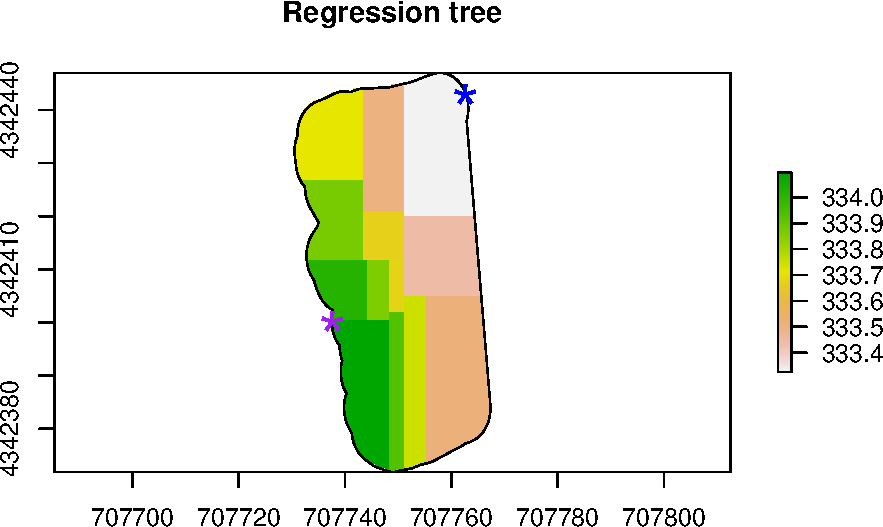
\includegraphics{_main_files/figure-latex/unnamed-chunk-20-1.pdf}

\hypertarget{support-vector-regression}{%
\subsection{4. Support vector regression}\label{support-vector-regression}}

\begin{Shaded}
\begin{Highlighting}[]
\CommentTok{\# Try support vector regression (or machine)!}
\FunctionTok{library}\NormalTok{(e1071)}
\NormalTok{m1 }\OtherTok{\textless{}{-}} \FunctionTok{svm}\NormalTok{(elev}\SpecialCharTok{\textasciitilde{}}\NormalTok{s1}\SpecialCharTok{+}\NormalTok{s2,}\AttributeTok{data=}\NormalTok{df.elev)}

\CommentTok{\# Make raster of study area to be able to map predictions from m1}
\NormalTok{rl.E.y\_svr }\OtherTok{\textless{}{-}} \FunctionTok{raster}\NormalTok{(,}\AttributeTok{nrow=}\DecValTok{100}\NormalTok{,}\AttributeTok{ncols=}\DecValTok{100}\NormalTok{,}\AttributeTok{ext=}\FunctionTok{extent}\NormalTok{(sf.study.area.utm),}\AttributeTok{crs=}\FunctionTok{crs}\NormalTok{(sf.study.area.utm))}
\CommentTok{\# Make data.frame to be able to make predictions at each pixel (cell of raster)}
\NormalTok{df.pred }\OtherTok{\textless{}{-}} \FunctionTok{data.frame}\NormalTok{(}\AttributeTok{elev =} \ConstantTok{NA}\NormalTok{,}
                      \AttributeTok{s1 =} \FunctionTok{xyFromCell}\NormalTok{(rl.E.y\_svr,}\AttributeTok{cell=}\DecValTok{1}\SpecialCharTok{:}\FunctionTok{length}\NormalTok{(rl.E.y\_svr[]))[,}\DecValTok{1}\NormalTok{],}
                      \AttributeTok{s2 =} \FunctionTok{xyFromCell}\NormalTok{(rl.E.y\_svr,}\AttributeTok{cell=}\DecValTok{1}\SpecialCharTok{:}\FunctionTok{length}\NormalTok{(rl.E.y\_svr[]))[,}\DecValTok{2}\NormalTok{])}

\CommentTok{\# Make spatial predictions at each pixel}
\NormalTok{df.pred}\SpecialCharTok{$}\NormalTok{elev }\OtherTok{\textless{}{-}} \FunctionTok{predict}\NormalTok{(m1,df.pred[,}\DecValTok{2}\SpecialCharTok{:}\DecValTok{3}\NormalTok{])}

\CommentTok{\# View first 6 rows of predictions}
\FunctionTok{head}\NormalTok{(df.pred) }
\end{Highlighting}
\end{Shaded}

\begin{verbatim}
##       elev       s1      s2
## 1 333.7520 707730.7 4342447
## 2 333.7524 707731.1 4342447
## 3 333.7522 707731.4 4342447
## 4 333.7515 707731.8 4342447
## 5 333.7500 707732.2 4342447
## 6 333.7479 707732.5 4342447
\end{verbatim}

\begin{Shaded}
\begin{Highlighting}[]
\CommentTok{\# Fill raster file with predictions }
\NormalTok{rl.E.y\_svr[] }\OtherTok{\textless{}{-}} \FunctionTok{c}\NormalTok{(df.pred}\SpecialCharTok{$}\NormalTok{elev)}

\NormalTok{rl.E.y\_svr }\OtherTok{\textless{}{-}} \FunctionTok{mask}\NormalTok{(rl.E.y\_svr,sf.study.area.utm)}

\CommentTok{\# Estimate coordinates and amount of maximum elevation}
\FunctionTok{xyFromCell}\NormalTok{(rl.E.y\_svr,}\AttributeTok{cell=}\FunctionTok{which.max}\NormalTok{(rl.E.y\_svr[]))}
\end{Highlighting}
\end{Shaded}

\begin{verbatim}
##           x       y
## [1,] 707744 4342389
\end{verbatim}

\begin{Shaded}
\begin{Highlighting}[]
\NormalTok{rl.E.y\_svr[}\FunctionTok{which.max}\NormalTok{(rl.E.y\_svr[])]}
\end{Highlighting}
\end{Shaded}

\begin{verbatim}
## [1] 334.1314
\end{verbatim}

\begin{Shaded}
\begin{Highlighting}[]
\CommentTok{\# Plot estimate coordinates of maximum elevation}
\NormalTok{\{}\FunctionTok{plot}\NormalTok{(rl.E.y\_svr, }\AttributeTok{main =} \StringTok{"Support vector regression"}\NormalTok{) }\CommentTok{\# Plot map of predictions}
\FunctionTok{plot}\NormalTok{(sf.study.area.utm,}\AttributeTok{add=}\ConstantTok{TRUE}\NormalTok{)}
\FunctionTok{points}\NormalTok{(}\FunctionTok{xyFromCell}\NormalTok{(rl.E.y\_svr,}\AttributeTok{cell=}\FunctionTok{which.max}\NormalTok{(rl.E.y\_svr[])),}\AttributeTok{col=}\StringTok{"purple"}\NormalTok{,}\AttributeTok{pch=}\StringTok{"*"}\NormalTok{,}\AttributeTok{cex=}\DecValTok{3}\NormalTok{)}
\FunctionTok{points}\NormalTok{(}\FunctionTok{xyFromCell}\NormalTok{(rl.E.y\_lin,}\AttributeTok{cell=}\FunctionTok{which.min}\NormalTok{(rl.E.y\_lin[])),}\AttributeTok{col=}\StringTok{"blue"}\NormalTok{,}\AttributeTok{pch=}\StringTok{"*"}\NormalTok{,}\AttributeTok{cex=}\DecValTok{3}\NormalTok{)\}}
\end{Highlighting}
\end{Shaded}

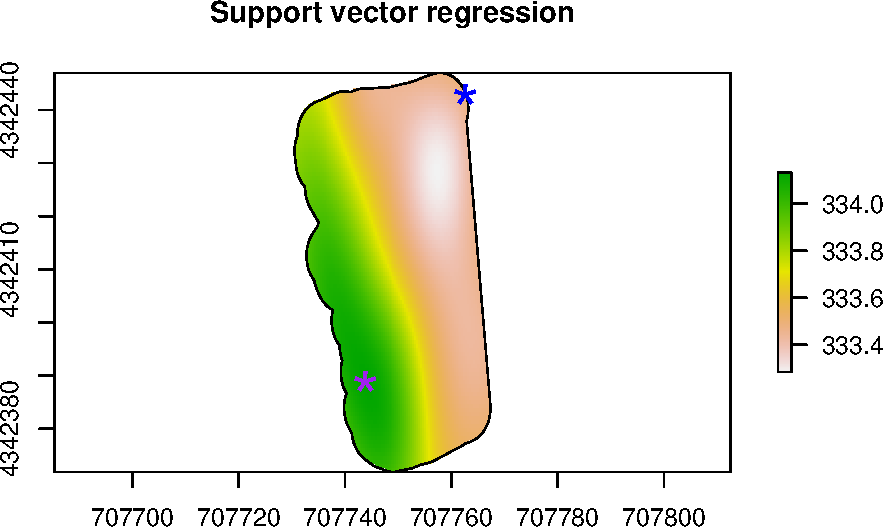
\includegraphics{_main_files/figure-latex/unnamed-chunk-21-1.pdf}

\hypertarget{boosted-regession-tree}{%
\subsection{5. Boosted regession tree}\label{boosted-regession-tree}}

\begin{Shaded}
\begin{Highlighting}[]
\CommentTok{\# Try boosted regression tree!}
\FunctionTok{library}\NormalTok{(gbm)}
\NormalTok{m1 }\OtherTok{\textless{}{-}} \FunctionTok{gbm}\NormalTok{(elev}\SpecialCharTok{\textasciitilde{}}\NormalTok{s1}\SpecialCharTok{+}\NormalTok{s2,}\AttributeTok{data=}\NormalTok{df.elev)}
\end{Highlighting}
\end{Shaded}

\begin{verbatim}
## Distribution not specified, assuming gaussian ...
\end{verbatim}

\begin{Shaded}
\begin{Highlighting}[]
\CommentTok{\# Make raster of study area to be able to map predictions from m1}
\NormalTok{rl.E.y\_gbm }\OtherTok{\textless{}{-}} \FunctionTok{raster}\NormalTok{(,}\AttributeTok{nrow=}\DecValTok{100}\NormalTok{,}\AttributeTok{ncols=}\DecValTok{100}\NormalTok{,}\AttributeTok{ext=}\FunctionTok{extent}\NormalTok{(sf.study.area.utm),}\AttributeTok{crs=}\FunctionTok{crs}\NormalTok{(sf.study.area.utm))}
\CommentTok{\# Make data.frame to be able to make predictions at each pixel (cell of raster)}
\NormalTok{df.pred }\OtherTok{\textless{}{-}} \FunctionTok{data.frame}\NormalTok{(}\AttributeTok{elev =} \ConstantTok{NA}\NormalTok{,}
                      \AttributeTok{s1 =} \FunctionTok{xyFromCell}\NormalTok{(rl.E.y\_gbm,}\AttributeTok{cell=}\DecValTok{1}\SpecialCharTok{:}\FunctionTok{length}\NormalTok{(rl.E.y\_gbm[]))[,}\DecValTok{1}\NormalTok{],}
                      \AttributeTok{s2 =} \FunctionTok{xyFromCell}\NormalTok{(rl.E.y\_gbm,}\AttributeTok{cell=}\DecValTok{1}\SpecialCharTok{:}\FunctionTok{length}\NormalTok{(rl.E.y\_gbm[]))[,}\DecValTok{2}\NormalTok{])}

\CommentTok{\# Make spatial predictions at each pixel}
\NormalTok{df.pred}\SpecialCharTok{$}\NormalTok{elev }\OtherTok{\textless{}{-}} \FunctionTok{predict}\NormalTok{(m1,df.pred[,}\DecValTok{2}\SpecialCharTok{:}\DecValTok{3}\NormalTok{])}

\CommentTok{\# View first 6 rows of predictions}
\FunctionTok{head}\NormalTok{(df.pred) }
\end{Highlighting}
\end{Shaded}

\begin{verbatim}
##       elev       s1      s2
## 1 333.8019 707730.7 4342447
## 2 333.8019 707731.1 4342447
## 3 333.8019 707731.4 4342447
## 4 333.8019 707731.8 4342447
## 5 333.8019 707732.2 4342447
## 6 333.8019 707732.5 4342447
\end{verbatim}

\begin{Shaded}
\begin{Highlighting}[]
\CommentTok{\# Fill raster file with predictions }
\NormalTok{rl.E.y\_gbm[] }\OtherTok{\textless{}{-}} \FunctionTok{c}\NormalTok{(df.pred}\SpecialCharTok{$}\NormalTok{elev)}

\NormalTok{rl.E.y\_gbm }\OtherTok{\textless{}{-}} \FunctionTok{mask}\NormalTok{(rl.E.y\_gbm,sf.study.area.utm)}

\CommentTok{\# Estimate coordinates and amount of maximum elevation}
\FunctionTok{xyFromCell}\NormalTok{(rl.E.y\_gbm,}\AttributeTok{cell=}\FunctionTok{which.max}\NormalTok{(rl.E.y\_gbm[]))}
\end{Highlighting}
\end{Shaded}

\begin{verbatim}
##             x       y
## [1,] 707739.5 4342392
\end{verbatim}

\begin{Shaded}
\begin{Highlighting}[]
\NormalTok{rl.E.y\_gbm[}\FunctionTok{which.max}\NormalTok{(rl.E.y\_gbm[])]}
\end{Highlighting}
\end{Shaded}

\begin{verbatim}
## [1] 334.1898
\end{verbatim}

\begin{Shaded}
\begin{Highlighting}[]
\CommentTok{\# Plot estimate coordinates of maximum elevation}
\NormalTok{\{}\FunctionTok{plot}\NormalTok{(rl.E.y\_gbm, }\AttributeTok{main =} \StringTok{"Boosted regression tree"}\NormalTok{) }\CommentTok{\# Plot map of predictions}
\FunctionTok{plot}\NormalTok{(sf.study.area.utm,}\AttributeTok{add=}\ConstantTok{TRUE}\NormalTok{)}
\FunctionTok{points}\NormalTok{(}\FunctionTok{xyFromCell}\NormalTok{(rl.E.y\_gbm,}\AttributeTok{cell=}\FunctionTok{which.max}\NormalTok{(rl.E.y\_gbm[])),}\AttributeTok{col=}\StringTok{"purple"}\NormalTok{,}\AttributeTok{pch=}\StringTok{"*"}\NormalTok{,}\AttributeTok{cex=}\DecValTok{3}\NormalTok{)}
\FunctionTok{points}\NormalTok{(}\FunctionTok{xyFromCell}\NormalTok{(rl.E.y\_lin,}\AttributeTok{cell=}\FunctionTok{which.min}\NormalTok{(rl.E.y\_lin[])),}\AttributeTok{col=}\StringTok{"blue"}\NormalTok{,}\AttributeTok{pch=}\StringTok{"*"}\NormalTok{,}\AttributeTok{cex=}\DecValTok{3}\NormalTok{)\}}
\end{Highlighting}
\end{Shaded}

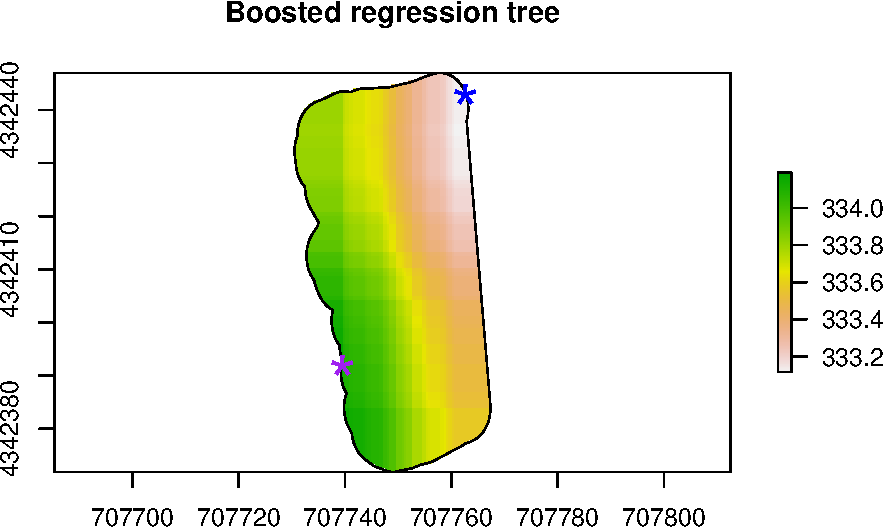
\includegraphics{_main_files/figure-latex/unnamed-chunk-22-1.pdf}

\hypertarget{activity-3}{%
\chapter{Activity 3}\label{activity-3}}

\hypertarget{libraries-1}{%
\section{Libraries}\label{libraries-1}}

\begin{Shaded}
\begin{Highlighting}[]
\FunctionTok{library}\NormalTok{(sf)}
\FunctionTok{library}\NormalTok{(sp)}
\FunctionTok{library}\NormalTok{(raster)}
\FunctionTok{library}\NormalTok{(mgcv)}
\FunctionTok{library}\NormalTok{(plotrix)}
\FunctionTok{library}\NormalTok{(gstat)}
\FunctionTok{library}\NormalTok{(tidyverse)}
\end{Highlighting}
\end{Shaded}

\hypertarget{english-grain-aphid-data}{%
\section{English grain Aphid Data}\label{english-grain-aphid-data}}

\begin{Shaded}
\begin{Highlighting}[]
\NormalTok{url }\OtherTok{\textless{}{-}} \StringTok{"https://www.dropbox.com/scl/fi/9ymxt900s77uq50ca6dgc/Enders{-}et{-}al.{-}2018{-}data.csv?rlkey=0rxjwleenhgu0gvzow5p0x9xf\&dl=1"}
\NormalTok{df1 }\OtherTok{\textless{}{-}} \FunctionTok{read.csv}\NormalTok{(url)}
\NormalTok{df1 }\OtherTok{\textless{}{-}}\NormalTok{ df1[,}\FunctionTok{c}\NormalTok{(}\DecValTok{2}\NormalTok{,}\DecValTok{8}\SpecialCharTok{:}\DecValTok{10}\NormalTok{)] }\CommentTok{\# Keep only the data on English grain aphid}
\FunctionTok{hist}\NormalTok{(df1}\SpecialCharTok{$}\NormalTok{EGA)}
\end{Highlighting}
\end{Shaded}

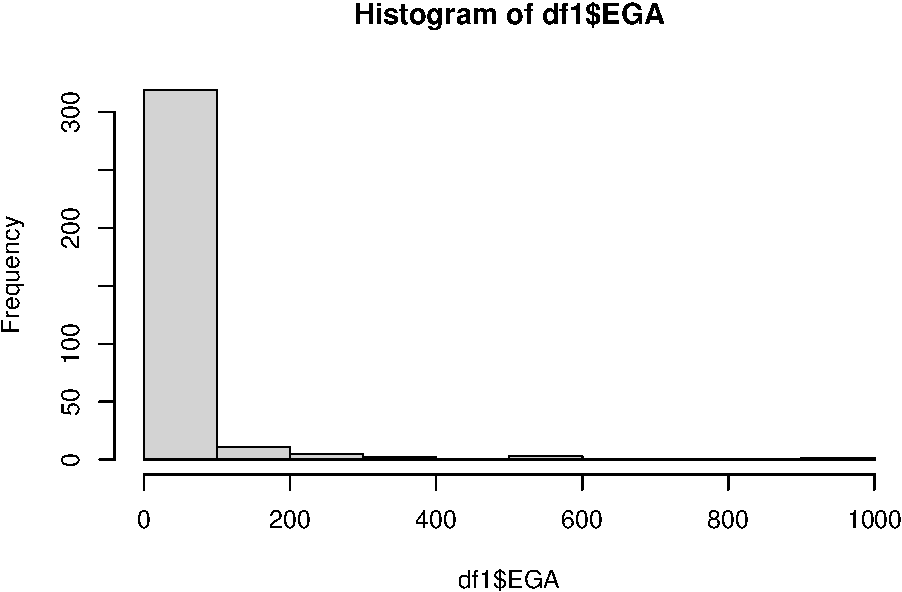
\includegraphics{_main_files/figure-latex/unnamed-chunk-24-1.pdf}

\hypertarget{kansas}{%
\section{Kansas}\label{kansas}}

\begin{Shaded}
\begin{Highlighting}[]
\CommentTok{\# Download shapefile of Kansas from census.gov}
\FunctionTok{download.file}\NormalTok{(}\StringTok{"http://www2.census.gov/geo/tiger/GENZ2015/shp/cb\_2015\_us\_state\_20m.zip"}\NormalTok{, }\AttributeTok{destfile =} \StringTok{"states.zip"}\NormalTok{)}
\FunctionTok{unzip}\NormalTok{(}\StringTok{"states.zip"}\NormalTok{)}
\NormalTok{sf.us }\OtherTok{\textless{}{-}} \FunctionTok{st\_read}\NormalTok{(}\StringTok{"cb\_2015\_us\_state\_20m.shp"}\NormalTok{,}\AttributeTok{quiet =} \ConstantTok{TRUE}\NormalTok{)}
\NormalTok{sf.kansas }\OtherTok{\textless{}{-}}\NormalTok{ sf.us[}\DecValTok{48}\NormalTok{,}\DecValTok{6}\NormalTok{]}
\NormalTok{sf.kansas }\OtherTok{\textless{}{-}} \FunctionTok{as}\NormalTok{(sf.kansas, }\StringTok{\textquotesingle{}Spatial\textquotesingle{}}\NormalTok{)}
\FunctionTok{plot}\NormalTok{(sf.kansas,}\AttributeTok{main=}\StringTok{""}\NormalTok{,}\AttributeTok{col=}\StringTok{"white"}\NormalTok{)}
\end{Highlighting}
\end{Shaded}


\includegraphics{_main_files/figure-latex/unnamed-chunk-25-1.pdf}

\hypertarget{spatial-df}{%
\chapter{Spatial DF}\label{spatial-df}}

\begin{Shaded}
\begin{Highlighting}[]
\CommentTok{\# Make SpatialPoints data frame}
\NormalTok{pts.sample }\OtherTok{\textless{}{-}} \FunctionTok{data.frame}\NormalTok{(}\AttributeTok{long =}\NormalTok{ df1}\SpecialCharTok{$}\NormalTok{long, }\AttributeTok{lat =}\NormalTok{ df1}\SpecialCharTok{$}\NormalTok{lat, }
                         \AttributeTok{count =}\NormalTok{ df1}\SpecialCharTok{$}\NormalTok{EGA)}
\FunctionTok{coordinates}\NormalTok{(pts.sample) }\OtherTok{=}\ErrorTok{\textasciitilde{}}\NormalTok{ long }\SpecialCharTok{+}\NormalTok{ lat}
\FunctionTok{proj4string}\NormalTok{(pts.sample) }\OtherTok{\textless{}{-}} \FunctionTok{CRS}\NormalTok{(}\StringTok{"+proj=longlat +datum=WGS84 +no\_defs +ellps=WGS84 +towgs84=0,0,0"}\NormalTok{)}
\end{Highlighting}
\end{Shaded}

\hypertarget{viz-count}{%
\chapter{Viz count}\label{viz-count}}

\begin{Shaded}
\begin{Highlighting}[]
\CommentTok{\# Plot counts of Bird cherry{-}oat aphid}
\FunctionTok{par}\NormalTok{(}\AttributeTok{mar=}\FunctionTok{c}\NormalTok{(}\FloatTok{5.1}\NormalTok{, }\FloatTok{4.1}\NormalTok{, }\FloatTok{4.1}\NormalTok{, }\FloatTok{8.1}\NormalTok{), }\AttributeTok{xpd=}\ConstantTok{TRUE}\NormalTok{)}
\FunctionTok{plot}\NormalTok{(sf.kansas,}\AttributeTok{main=}\StringTok{"Abundance of English Grain Aphid"}\NormalTok{)}
\FunctionTok{points}\NormalTok{(pts.sample[,}\DecValTok{1}\NormalTok{],}\AttributeTok{col=}\FunctionTok{rgb}\NormalTok{(}\FloatTok{0.4}\NormalTok{,}\FloatTok{0.8}\NormalTok{,}\FloatTok{0.5}\NormalTok{,}\FloatTok{0.9}\NormalTok{),}\AttributeTok{pch=}\FunctionTok{ifelse}\NormalTok{(pts.sample}\SpecialCharTok{$}\NormalTok{count}\SpecialCharTok{\textgreater{}}\DecValTok{0}\NormalTok{,}\DecValTok{20}\NormalTok{,}\DecValTok{4}\NormalTok{),}\AttributeTok{cex=}\NormalTok{pts.sample}\SpecialCharTok{$}\NormalTok{count}\SpecialCharTok{/}\DecValTok{50}\FloatTok{+0.5}\NormalTok{)}
\FunctionTok{legend}\NormalTok{(}\StringTok{"right"}\NormalTok{,}\AttributeTok{inset=}\FunctionTok{c}\NormalTok{(}\SpecialCharTok{{-}}\FloatTok{0.25}\NormalTok{,}\DecValTok{0}\NormalTok{),}\AttributeTok{legend =} \FunctionTok{c}\NormalTok{(}\DecValTok{0}\NormalTok{,}\DecValTok{1}\NormalTok{,}\DecValTok{10}\NormalTok{,}\DecValTok{20}\NormalTok{,}\DecValTok{40}\NormalTok{,}\DecValTok{60}\NormalTok{), }\AttributeTok{bty =} \StringTok{"n"}\NormalTok{, }\AttributeTok{text.col =} \StringTok{"black"}\NormalTok{, }
       \AttributeTok{pch=}\FunctionTok{c}\NormalTok{(}\DecValTok{4}\NormalTok{,}\DecValTok{20}\NormalTok{,}\DecValTok{20}\NormalTok{,}\DecValTok{20}\NormalTok{,}\DecValTok{20}\NormalTok{,}\DecValTok{20}\NormalTok{), }\AttributeTok{cex=}\FloatTok{1.3}\NormalTok{,}\AttributeTok{pt.cex=}\FunctionTok{c}\NormalTok{(}\DecValTok{0}\NormalTok{,}\DecValTok{1}\NormalTok{,}\DecValTok{10}\NormalTok{,}\DecValTok{20}\NormalTok{,}\DecValTok{40}\NormalTok{,}\DecValTok{60}\NormalTok{)}\SpecialCharTok{/}\DecValTok{50}\FloatTok{+0.5}\NormalTok{,}\AttributeTok{col=}\FunctionTok{rgb}\NormalTok{(}\FloatTok{0.4}\NormalTok{,}\FloatTok{0.8}\NormalTok{,}\FloatTok{0.5}\NormalTok{,}\FloatTok{0.9}\NormalTok{))}
\end{Highlighting}
\end{Shaded}

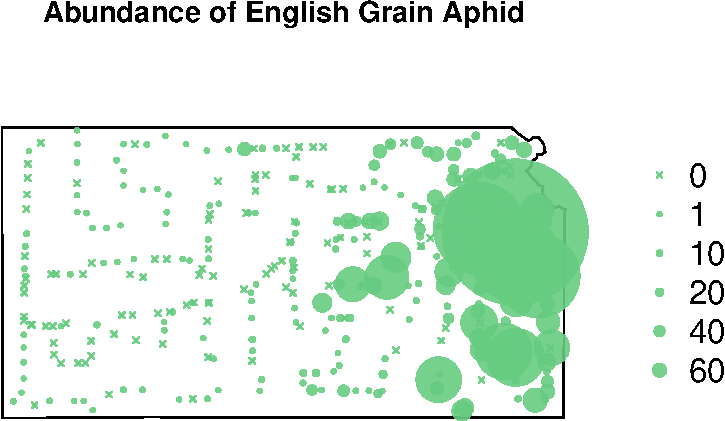
\includegraphics{_main_files/figure-latex/unnamed-chunk-27-1.pdf}

\begin{Shaded}
\begin{Highlighting}[]
\CommentTok{\# Maximum observed: 940 individuals}
\end{Highlighting}
\end{Shaded}

\hypertarget{land-cover-data}{%
\section{Land Cover data}\label{land-cover-data}}

\begin{Shaded}
\begin{Highlighting}[]
\CommentTok{\# Download National Land Cover Database}
\CommentTok{\#url.nlcd \textless{}{-} "https://www.dropbox.com/scl/fi/ew7yzm93aes7l8l37cn65/KS\_2011\_NLCD.img?rlkey=60ahyvxhq18gt0yr47tuq5fig\&dl=1"}
\CommentTok{\#rl.nlcd2011 \textless{}{-} raster(url.nlcd)}
\CommentTok{\#saveRDS(rl.nlcd2011, "rl.nlcd2011.RDS")}

\NormalTok{rl.nlcd2011 }\OtherTok{\textless{}{-}} \FunctionTok{readRDS}\NormalTok{(}\StringTok{"../rl.nlcd2011.RDS"}\NormalTok{)}
\FunctionTok{plot}\NormalTok{(rl.nlcd2011)}
\end{Highlighting}
\end{Shaded}

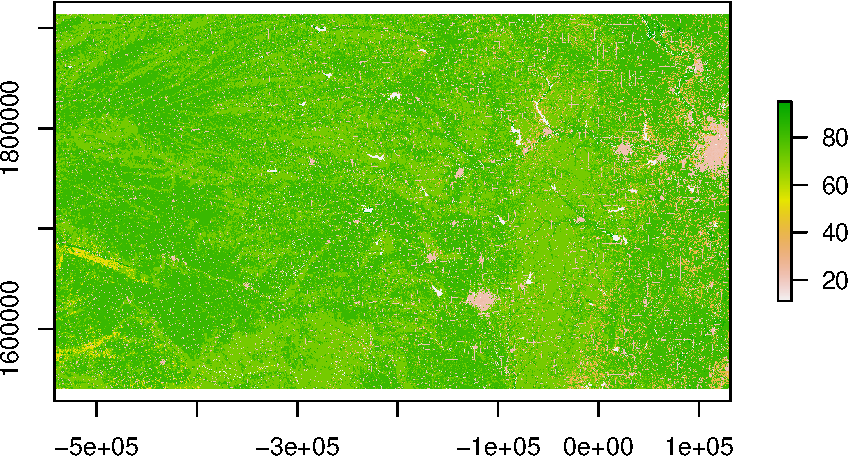
\includegraphics{_main_files/figure-latex/unnamed-chunk-28-1.pdf}

\hypertarget{raster-w-grassland}{%
\section{Raster w grassland}\label{raster-w-grassland}}

\begin{Shaded}
\begin{Highlighting}[]
\CommentTok{\# Make raster file that contains pixels with value of 1 if grassland and }
\CommentTok{\# zero if other type of land cover.}
\CommentTok{\# NLCD legend can be found here: https://www.mrlc.gov/data/legends/national{-}land{-}cover{-}database{-}2011{-}nlcd2011{-}legend}
\CommentTok{\#rl.nlcd.grass \textless{}{-} rl.nlcd2011}
\CommentTok{\#rl.nlcd.grass[] \textless{}{-} ifelse(rl.nlcd.grass[]==71,1,0)}

\CommentTok{\#saveRDS(rl.nlcd.grass, "rl.nlcd.grass.RDS")}

\NormalTok{rl.nlcd.grass }\OtherTok{\textless{}{-}} \FunctionTok{readRDS}\NormalTok{(}\StringTok{"../rl.nlcd.grass.RDS"}\NormalTok{)}

\FunctionTok{plot}\NormalTok{(rl.nlcd.grass)}
\end{Highlighting}
\end{Shaded}

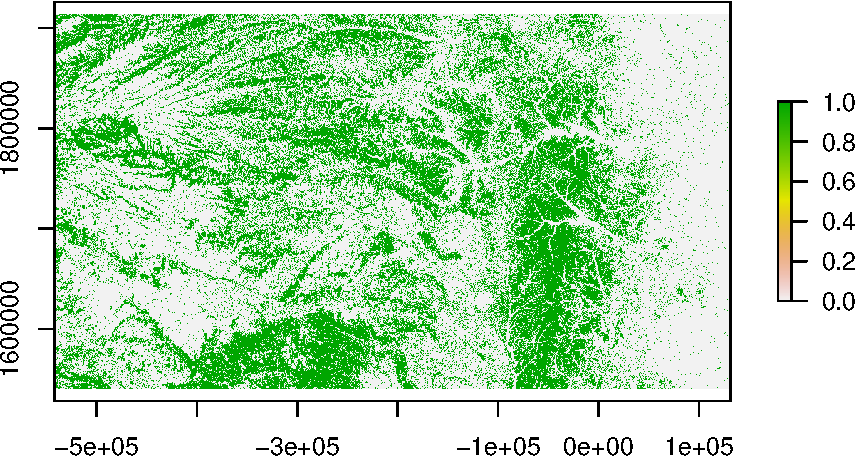
\includegraphics{_main_files/figure-latex/unnamed-chunk-29-1.pdf}

\hypertarget{grassland-within-5-km-of-sampling}{%
\chapter{Grassland within 5 km of sampling}\label{grassland-within-5-km-of-sampling}}

\begin{Shaded}
\begin{Highlighting}[]
\CommentTok{\# Calculate percentage of land area that is grassland withing 5 km of sampled location}
\NormalTok{df1}\SpecialCharTok{$}\NormalTok{grass.perc }\OtherTok{\textless{}{-}} \FunctionTok{unlist}\NormalTok{(}\FunctionTok{lapply}\NormalTok{(raster}\SpecialCharTok{::}\FunctionTok{extract}\NormalTok{(rl.nlcd.grass,pts.sample,}\AttributeTok{buffer=}\DecValTok{5000}\NormalTok{),mean))}\SpecialCharTok{*}\DecValTok{100}

\FunctionTok{hist}\NormalTok{(df1}\SpecialCharTok{$}\NormalTok{grass.perc,}\AttributeTok{col=}\StringTok{"grey"}\NormalTok{,}\AttributeTok{main=}\StringTok{""}\NormalTok{,}\AttributeTok{xlab=}\StringTok{"\% grassland within }\SpecialCharTok{\textbackslash{}n}\StringTok{5 km at sample location"}\NormalTok{)}
\end{Highlighting}
\end{Shaded}

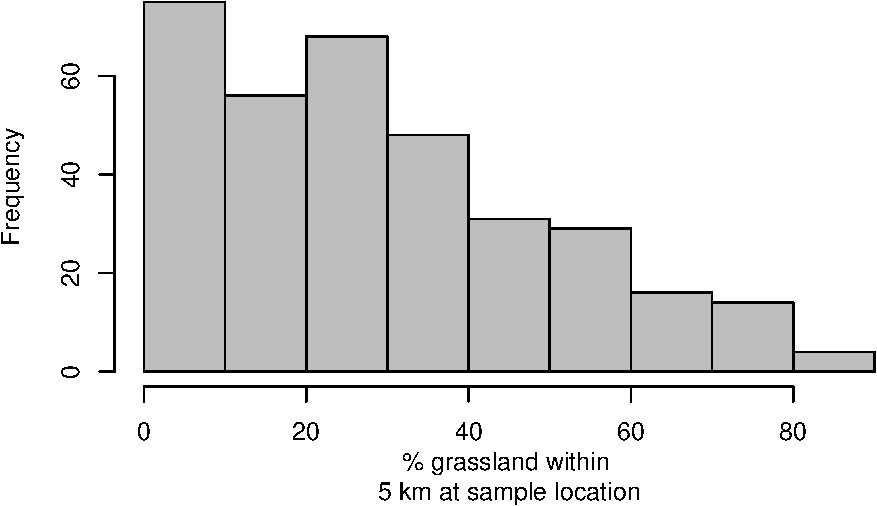
\includegraphics{_main_files/figure-latex/unnamed-chunk-30-1.pdf}

\hypertarget{run-models}{%
\chapter{Run models}\label{run-models}}

\begin{Shaded}
\begin{Highlighting}[]
\NormalTok{sample }\OtherTok{=} \FunctionTok{sample}\NormalTok{(}\FunctionTok{c}\NormalTok{(}\ConstantTok{TRUE}\NormalTok{,}\ConstantTok{FALSE}\NormalTok{), }\FunctionTok{nrow}\NormalTok{(df1), }\AttributeTok{replace=}\ConstantTok{TRUE}\NormalTok{, }\AttributeTok{prob=}\FunctionTok{c}\NormalTok{(}\FloatTok{0.6}\NormalTok{,}\FloatTok{0.4}\NormalTok{)) }
\NormalTok{train }\OtherTok{=}\NormalTok{ df1[sample,]}
\NormalTok{test }\OtherTok{=}\NormalTok{ df1[}\SpecialCharTok{!}\NormalTok{sample,]}

\CommentTok{\# Fit different spatio{-}temporal models to Bird cherry{-}oat aphid abundance data }
\NormalTok{m1 }\OtherTok{\textless{}{-}} \FunctionTok{gam}\NormalTok{(EGA }\SpecialCharTok{\textasciitilde{}}\NormalTok{ grass.perc }\SpecialCharTok{+} \FunctionTok{as.factor}\NormalTok{(year) }\SpecialCharTok{+} \FunctionTok{s}\NormalTok{(long,lat, }\AttributeTok{bs =} \StringTok{"gp"}\NormalTok{), }
          \AttributeTok{family =} \FunctionTok{poisson}\NormalTok{(}\AttributeTok{link =} \StringTok{"log"}\NormalTok{), }\AttributeTok{data =}\NormalTok{ train)}
\FunctionTok{summary}\NormalTok{(m1)}
\end{Highlighting}
\end{Shaded}

\begin{verbatim}
## 
## Family: poisson 
## Link function: log 
## 
## Formula:
## EGA ~ grass.perc + as.factor(year) + s(long, lat, bs = "gp")
## 
## Parametric coefficients:
##                     Estimate Std. Error z value Pr(>|z|)    
## (Intercept)         -3.27808    0.38353  -8.547   <2e-16 ***
## grass.perc          -0.01247    0.00125  -9.975   <2e-16 ***
## as.factor(year)2015  5.65719    0.37834  14.953   <2e-16 ***
## ---
## Signif. codes:  0 '***' 0.001 '**' 0.01 '*' 0.05 '.' 0.1 ' ' 1
## 
## Approximate significance of smooth terms:
##               edf Ref.df Chi.sq p-value    
## s(long,lat) 31.95     32   4805  <2e-16 ***
## ---
## Signif. codes:  0 '***' 0.001 '**' 0.01 '*' 0.05 '.' 0.1 ' ' 1
## 
## R-sq.(adj) =  0.439   Deviance explained = 72.5%
## UBRE =  25.17  Scale est. = 1         n = 206
\end{verbatim}

\begin{Shaded}
\begin{Highlighting}[]
\NormalTok{m2 }\OtherTok{\textless{}{-}} \FunctionTok{gam}\NormalTok{(EGA }\SpecialCharTok{\textasciitilde{}}\NormalTok{ grass.perc }\SpecialCharTok{+} \FunctionTok{as.factor}\NormalTok{(year) }\SpecialCharTok{+} \FunctionTok{s}\NormalTok{(long,lat, }\AttributeTok{bs =} \StringTok{"gp"}\NormalTok{), }
          \AttributeTok{family =} \FunctionTok{nb}\NormalTok{(}\AttributeTok{theta =} \ConstantTok{NULL}\NormalTok{,}\AttributeTok{link =} \StringTok{"log"}\NormalTok{), }\AttributeTok{data =}\NormalTok{ train)}
\FunctionTok{summary}\NormalTok{(m2)}
\end{Highlighting}
\end{Shaded}

\begin{verbatim}
## 
## Family: Negative Binomial(0.6) 
## Link function: log 
## 
## Formula:
## EGA ~ grass.perc + as.factor(year) + s(long, lat, bs = "gp")
## 
## Parametric coefficients:
##                      Estimate Std. Error z value Pr(>|z|)    
## (Intercept)         -2.792454   0.482367  -5.789 7.08e-09 ***
## grass.perc          -0.003721   0.005949  -0.626    0.532    
## as.factor(year)2015  5.442228   0.459096  11.854  < 2e-16 ***
## ---
## Signif. codes:  0 '***' 0.001 '**' 0.01 '*' 0.05 '.' 0.1 ' ' 1
## 
## Approximate significance of smooth terms:
##               edf Ref.df Chi.sq p-value    
## s(long,lat) 6.439  8.532  230.6  <2e-16 ***
## ---
## Signif. codes:  0 '***' 0.001 '**' 0.01 '*' 0.05 '.' 0.1 ' ' 1
## 
## R-sq.(adj) =  0.242   Deviance explained =   68%
## -REML = 597.07  Scale est. = 1         n = 206
\end{verbatim}

\begin{Shaded}
\begin{Highlighting}[]
\NormalTok{m3 }\OtherTok{\textless{}{-}} \FunctionTok{gam}\NormalTok{(}\FunctionTok{list}\NormalTok{(EGA }\SpecialCharTok{\textasciitilde{}}\NormalTok{ grass.perc }\SpecialCharTok{+} \FunctionTok{as.factor}\NormalTok{(year) }\SpecialCharTok{+} \FunctionTok{s}\NormalTok{(long,lat, }\AttributeTok{bs =} \StringTok{"gp"}\NormalTok{), }\SpecialCharTok{\textasciitilde{}}\NormalTok{ grass.perc), }
          \AttributeTok{family =} \FunctionTok{ziplss}\NormalTok{(), }\AttributeTok{data =}\NormalTok{ train)}
\FunctionTok{summary}\NormalTok{(m3)}
\end{Highlighting}
\end{Shaded}

\begin{verbatim}
## 
## Family: ziplss 
## Link function: identity identity 
## 
## Formula:
## EGA ~ grass.perc + as.factor(year) + s(long, lat, bs = "gp")
## ~grass.perc
## 
## Parametric coefficients:
##                      Estimate Std. Error z value Pr(>|z|)    
## (Intercept)         -0.858658   0.538626  -1.594    0.111    
## grass.perc          -0.014579   0.001258 -11.589  < 2e-16 ***
## as.factor(year)2015  3.327181   0.530770   6.269 3.64e-10 ***
## (Intercept).1        0.065371   0.156736   0.417    0.677    
## grass.perc.1        -0.001425   0.004385  -0.325    0.745    
## ---
## Signif. codes:  0 '***' 0.001 '**' 0.01 '*' 0.05 '.' 0.1 ' ' 1
## 
## Approximate significance of smooth terms:
##              edf Ref.df Chi.sq p-value    
## s(long,lat) 31.3  31.67   3776  <2e-16 ***
## ---
## Signif. codes:  0 '***' 0.001 '**' 0.01 '*' 0.05 '.' 0.1 ' ' 1
## 
## Deviance explained = 63.7%
## -REML = 2998.4  Scale est. = 1         n = 206
\end{verbatim}

\begin{Shaded}
\begin{Highlighting}[]
\NormalTok{m4 }\OtherTok{\textless{}{-}} \FunctionTok{gam}\NormalTok{(EGA }\SpecialCharTok{\textasciitilde{}}\NormalTok{ grass.perc }\SpecialCharTok{+} \FunctionTok{as.factor}\NormalTok{(year) }\SpecialCharTok{+} \FunctionTok{s}\NormalTok{(long,lat, }\AttributeTok{bs =} \StringTok{"gp"}\NormalTok{), }
          \AttributeTok{family =} \FunctionTok{gaussian}\NormalTok{(}\AttributeTok{link=}\StringTok{"identity"}\NormalTok{), }\AttributeTok{data =}\NormalTok{ train)}
\FunctionTok{summary}\NormalTok{(m4)}
\end{Highlighting}
\end{Shaded}

\begin{verbatim}
## 
## Family: gaussian 
## Link function: identity 
## 
## Formula:
## EGA ~ grass.perc + as.factor(year) + s(long, lat, bs = "gp")
## 
## Parametric coefficients:
##                     Estimate Std. Error t value Pr(>|t|)    
## (Intercept)           2.5300    13.3708   0.189 0.850114    
## grass.perc           -0.1551     0.2592  -0.598 0.550313    
## as.factor(year)2015  40.8719    11.9772   3.412 0.000779 ***
## ---
## Signif. codes:  0 '***' 0.001 '**' 0.01 '*' 0.05 '.' 0.1 ' ' 1
## 
## Approximate significance of smooth terms:
##             edf Ref.df     F p-value    
## s(long,lat) 3.3  4.196 7.948 4.6e-06 ***
## ---
## Signif. codes:  0 '***' 0.001 '**' 0.01 '*' 0.05 '.' 0.1 ' ' 1
## 
## R-sq.(adj) =  0.182   Deviance explained = 20.3%
## GCV = 5330.1  Scale est. = 5167.1    n = 206
\end{verbatim}

\hypertarget{statistical-model}{%
\chapter{Statistical model}\label{statistical-model}}

\textbf{Model 1:}\\
\(Z=y_i\) where i is the year and goes from 2014 and 2015.\\
\strut \\
\([y_i|\lambda]=Poisson(\lambda)]\)\\
\strut \\
\(E(y_i)=e^{\beta_0+\beta1 \cdot X+\eta_s+\eta_t}\)\\
\strut \\
\(\eta_s \sim MVN(0,\Sigma)\)~\\
\textbf{Model 2:}\\
\(Z=y_i\) where i is the year and goes from 2014 and 2015.\\
\strut \\
\([y_i|r,p]=NB(r,p)]\)\\
\strut \\
\(E(y_i)=e^{\beta_0+\beta1 \cdot X+\eta_s+\eta_t}\)\\
\strut \\
\(\eta_s \sim MVN(0,\Sigma)\)~\\
\textbf{Model 3:}\\
\(Z=y_i\) where i is the year and goes from 2014 and 2015.\\
\strut \\
\([y_i|\pi,\lambda]=ZIP(\pi,\lambda)]\)\\
\strut \\
\(P(Y=0)=\pi+(1-\pi)e^{-\lambda}\)\\
\strut \\
\(P(Y=y_i)=(1-\pi)\cfrac{\lambda^{y_i}e^{-\lambda}}{y_i}\)\\
\strut \\
\(E(y_i)=e^{\beta_0+\beta1 \cdot X+\eta_s+\eta_t}\)\\
\strut \\
\(\eta_s \sim MVN(0,\Sigma)\)~\\
\textbf{Model 3:}\\
\(Z=y_i\) where i is the year and goes from 2014 and 2015.\\
\strut \\
\([y_i|\mu, \sigma^2]=Gaussian(\mu,\sigma^2)]\)\\
\strut \\
\(E(y_i)=e^{\beta_0+\beta1 \cdot X+\eta_s+\eta_t}\)\\
\strut \\
\(\eta_s \sim MVN(0,\Sigma)\)~

\begin{Shaded}
\begin{Highlighting}[]
\CommentTok{\# Examine regression coefficient estimates and 95\% CI}
\NormalTok{beta.}\FloatTok{1.}\NormalTok{hat }\OtherTok{\textless{}{-}} \FunctionTok{c}\NormalTok{(}\FunctionTok{coef}\NormalTok{(m1)[}\DecValTok{2}\NormalTok{],}\FunctionTok{coef}\NormalTok{(m2)[}\DecValTok{2}\NormalTok{],}\FunctionTok{coef}\NormalTok{(m3)[}\DecValTok{2}\NormalTok{],}\FunctionTok{coef}\NormalTok{(m4)[}\DecValTok{2}\NormalTok{])}
\NormalTok{beta.}\FloatTok{1.}\NormalTok{hat }\CommentTok{\# order is m1, m2 and m3}
\end{Highlighting}
\end{Shaded}

\begin{verbatim}
##   grass.perc   grass.perc   grass.perc   grass.perc 
## -0.012465733 -0.003721275 -0.014578533 -0.155076059
\end{verbatim}

\begin{Shaded}
\begin{Highlighting}[]
\FunctionTok{exp}\NormalTok{(beta.}\FloatTok{1.}\NormalTok{hat[}\DecValTok{1}\SpecialCharTok{:}\DecValTok{3}\NormalTok{]}\SpecialCharTok{*}\DecValTok{0}\NormalTok{)}\SpecialCharTok{/}\FunctionTok{exp}\NormalTok{(beta.}\FloatTok{1.}\NormalTok{hat[}\DecValTok{1}\SpecialCharTok{:}\DecValTok{3}\NormalTok{]}\SpecialCharTok{*}\DecValTok{100}\NormalTok{) }\CommentTok{\# Abundance at 0\% grassland/Abundance at 100\% grassland}
\end{Highlighting}
\end{Shaded}

\begin{verbatim}
## grass.perc grass.perc grass.perc 
##   3.478403   1.450818   4.296726
\end{verbatim}

\begin{Shaded}
\begin{Highlighting}[]
\NormalTok{ucl }\OtherTok{\textless{}{-}} \FunctionTok{c}\NormalTok{(}\FunctionTok{confint.default}\NormalTok{(m1,}\AttributeTok{parm=}\StringTok{"grass.perc"}\NormalTok{)[}\DecValTok{2}\NormalTok{],}
         \FunctionTok{confint.default}\NormalTok{(m2,}\AttributeTok{parm=}\StringTok{"grass.perc"}\NormalTok{)[}\DecValTok{2}\NormalTok{],}
         \FunctionTok{confint.default}\NormalTok{(m3,}\AttributeTok{parm=}\StringTok{"grass.perc"}\NormalTok{)[}\DecValTok{2}\NormalTok{],}
         \FunctionTok{confint.default}\NormalTok{(m4,}\AttributeTok{parm=}\StringTok{"grass.perc"}\NormalTok{)[}\DecValTok{2}\NormalTok{])}

\NormalTok{lcl }\OtherTok{\textless{}{-}} \FunctionTok{c}\NormalTok{(}\FunctionTok{confint.default}\NormalTok{(m1,}\AttributeTok{parm=}\StringTok{"grass.perc"}\NormalTok{)[}\DecValTok{1}\NormalTok{],}
         \FunctionTok{confint.default}\NormalTok{(m2,}\AttributeTok{parm=}\StringTok{"grass.perc"}\NormalTok{)[}\DecValTok{1}\NormalTok{],}
         \FunctionTok{confint.default}\NormalTok{(m3,}\AttributeTok{parm=}\StringTok{"grass.perc"}\NormalTok{)[}\DecValTok{1}\NormalTok{],}
         \FunctionTok{confint.default}\NormalTok{(m4,}\AttributeTok{parm=}\StringTok{"grass.perc"}\NormalTok{)[}\DecValTok{1}\NormalTok{])}

\FunctionTok{par}\NormalTok{(}\AttributeTok{mar=}\FunctionTok{c}\NormalTok{(}\DecValTok{4}\NormalTok{,}\DecValTok{7}\NormalTok{,}\DecValTok{1}\NormalTok{,}\DecValTok{1}\NormalTok{))}
\FunctionTok{plotCI}\NormalTok{(}\FunctionTok{c}\NormalTok{(}\DecValTok{1}\SpecialCharTok{:}\DecValTok{4}\NormalTok{), beta.}\FloatTok{1.}\NormalTok{hat, }\AttributeTok{ui=}\NormalTok{ucl, }\AttributeTok{li=}\NormalTok{lcl,}\AttributeTok{pch=}\DecValTok{20}\NormalTok{,}\AttributeTok{xaxt=}\StringTok{"n"}\NormalTok{,}\AttributeTok{xlab=}\StringTok{""}\NormalTok{,}\AttributeTok{ylab=}\StringTok{"Estimated regression coefficient }\SpecialCharTok{\textbackslash{}n}\StringTok{ (\% grass within 5km)"}\NormalTok{)}
\FunctionTok{lines}\NormalTok{(}\FunctionTok{c}\NormalTok{(}\DecValTok{1}\NormalTok{,}\DecValTok{4}\NormalTok{),}\FunctionTok{c}\NormalTok{(}\DecValTok{0}\NormalTok{,}\DecValTok{0}\NormalTok{),}\AttributeTok{col=}\StringTok{"gold"}\NormalTok{,}\AttributeTok{lwd=}\DecValTok{3}\NormalTok{)}
\FunctionTok{axis}\NormalTok{(}\AttributeTok{at=}\FunctionTok{c}\NormalTok{(}\DecValTok{1}\SpecialCharTok{:}\DecValTok{4}\NormalTok{),}\AttributeTok{lab=}\FunctionTok{c}\NormalTok{(}\StringTok{"Pois"}\NormalTok{,}\StringTok{"NB"}\NormalTok{,}\StringTok{"ZIP"}\NormalTok{, }\StringTok{"gauss"}\NormalTok{),}\AttributeTok{side=}\DecValTok{1}\NormalTok{)}
\end{Highlighting}
\end{Shaded}

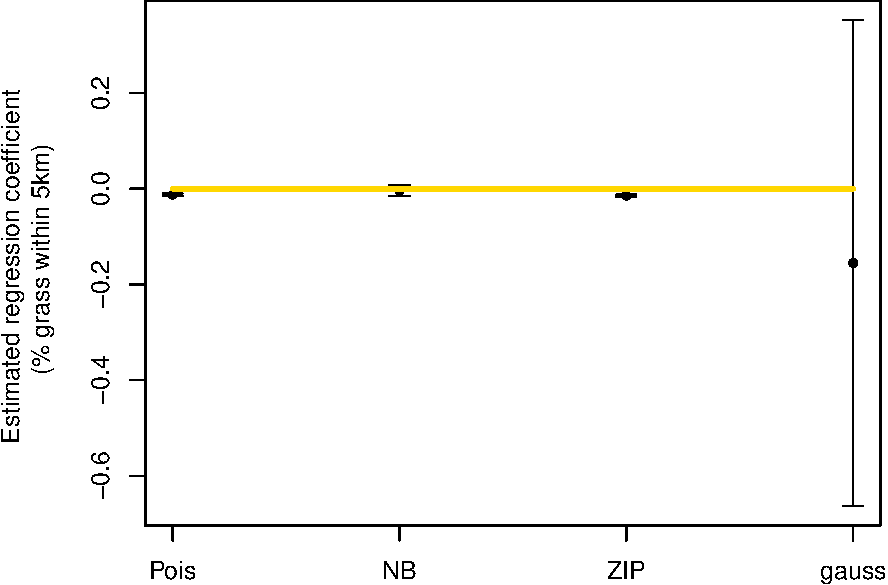
\includegraphics{_main_files/figure-latex/unnamed-chunk-32-1.pdf}

\begin{Shaded}
\begin{Highlighting}[]
\CommentTok{\# NB non{-}significant coefficient}
\CommentTok{\# Pois and ZIP coefficient different from 0}
\end{Highlighting}
\end{Shaded}

\hypertarget{compare-models}{%
\section{Compare models}\label{compare-models}}

\begin{Shaded}
\begin{Highlighting}[]
\CommentTok{\# Compare models using AIC (see pgs. 284{-}286 in Wikle et al. 2019)}
\FunctionTok{AIC}\NormalTok{(m1,m2,m3,m4)}
\end{Highlighting}
\end{Shaded}

\begin{verbatim}
##           df      AIC
## m1 34.948904 5944.996
## m2 11.696284 1188.827
## m3 36.445190 5757.906
## m4  7.300144 2354.119
\end{verbatim}

\hypertarget{concurvity}{%
\subsection{Concurvity}\label{concurvity}}

\begin{Shaded}
\begin{Highlighting}[]
\CommentTok{\# Model checking}
\CommentTok{\# See pg. 164 of Wikle et al. (2019) or }
\CommentTok{\# Hodges and Reich 2010 (https://www4.stat.ncsu.edu/\textasciitilde{}bjreich/papers/FixedEffectsYouLove.pdf)}
\FunctionTok{concurvity}\NormalTok{(m1)}
\end{Highlighting}
\end{Shaded}

\begin{verbatim}
##               para s(long,lat)
## worst    0.9098828  0.58252517
## observed 0.9098828  0.02028449
## estimate 0.9098828  0.03954218
\end{verbatim}

\begin{Shaded}
\begin{Highlighting}[]
\FunctionTok{concurvity}\NormalTok{(m2)}
\end{Highlighting}
\end{Shaded}

\begin{verbatim}
##               para s(long,lat)
## worst    0.9098828  0.58252517
## observed 0.9098828  0.03227996
## estimate 0.9098828  0.03954218
\end{verbatim}

\begin{Shaded}
\begin{Highlighting}[]
\FunctionTok{concurvity}\NormalTok{(m3)}
\end{Highlighting}
\end{Shaded}

\begin{verbatim}
##          para s(long,lat)
## worst       1  0.58653419
## observed    1  0.02024976
## estimate    1  0.04713506
\end{verbatim}

\begin{Shaded}
\begin{Highlighting}[]
\FunctionTok{concurvity}\NormalTok{(m4)}
\end{Highlighting}
\end{Shaded}

\begin{verbatim}
##               para s(long,lat)
## worst    0.9098828  0.58252517
## observed 0.9098828  0.07805267
## estimate 0.9098828  0.03954218
\end{verbatim}

\hypertarget{semivariogram-for-corr-resids}{%
\section{Semivariogram for corr resids}\label{semivariogram-for-corr-resids}}

\begin{Shaded}
\begin{Highlighting}[]
\CommentTok{\# Semivariogram to check for spatial autocorrelation among}
\CommentTok{\# residuals (see pg. 267 in Wikle et al. 2019 or}
\CommentTok{\# Wood 2017 pg. 364 Generalized additive models: an introduction with R)}
\NormalTok{vg1 }\OtherTok{\textless{}{-}} \FunctionTok{variogram}\NormalTok{(}\FunctionTok{residuals.gam}\NormalTok{(m1, }\AttributeTok{type =} \StringTok{"response"}\NormalTok{) }\SpecialCharTok{\textasciitilde{}} \DecValTok{1}\NormalTok{, }\AttributeTok{loc =} \SpecialCharTok{\textasciitilde{}}\NormalTok{long }\SpecialCharTok{+}
\NormalTok{                  lat, }\AttributeTok{data =}\NormalTok{ train)}
\FunctionTok{plot}\NormalTok{(vg1)}
\end{Highlighting}
\end{Shaded}

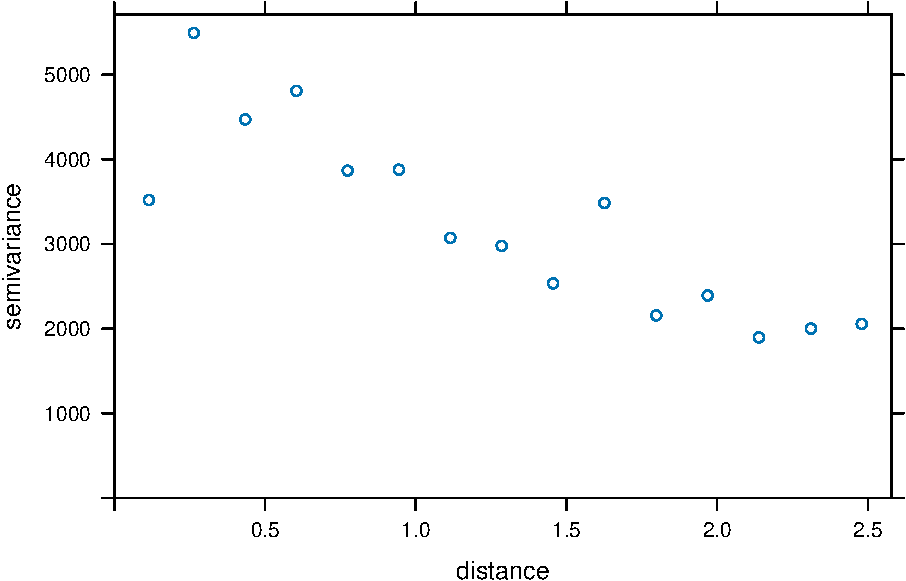
\includegraphics{_main_files/figure-latex/unnamed-chunk-35-1.pdf}

\begin{Shaded}
\begin{Highlighting}[]
\NormalTok{vg2 }\OtherTok{\textless{}{-}} \FunctionTok{variogram}\NormalTok{(}\FunctionTok{residuals.gam}\NormalTok{(m2, }\AttributeTok{type =} \StringTok{"response"}\NormalTok{) }\SpecialCharTok{\textasciitilde{}} \DecValTok{1}\NormalTok{, }\AttributeTok{loc =} \SpecialCharTok{\textasciitilde{}}\NormalTok{long }\SpecialCharTok{+}
\NormalTok{                  lat, }\AttributeTok{data =}\NormalTok{ train)}
\FunctionTok{plot}\NormalTok{(vg2)}
\end{Highlighting}
\end{Shaded}

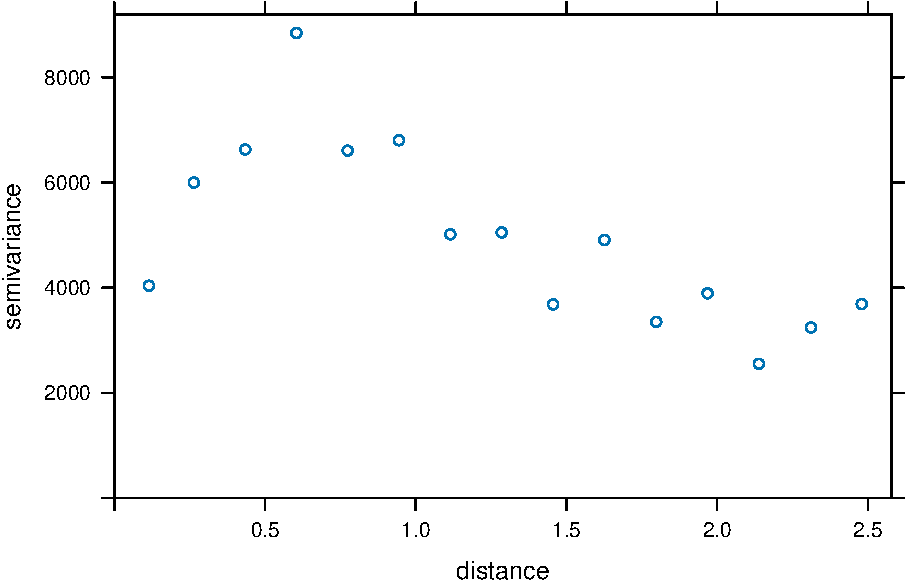
\includegraphics{_main_files/figure-latex/unnamed-chunk-35-2.pdf}

\begin{Shaded}
\begin{Highlighting}[]
\NormalTok{vg3 }\OtherTok{\textless{}{-}} \FunctionTok{variogram}\NormalTok{(}\FunctionTok{residuals.gam}\NormalTok{(m3, }\AttributeTok{type =} \StringTok{"response"}\NormalTok{) }\SpecialCharTok{\textasciitilde{}} \DecValTok{1}\NormalTok{, }\AttributeTok{loc =} \SpecialCharTok{\textasciitilde{}}\NormalTok{long }\SpecialCharTok{+}
\NormalTok{                  lat, }\AttributeTok{data =}\NormalTok{ train)}
\FunctionTok{plot}\NormalTok{(vg3)}
\end{Highlighting}
\end{Shaded}

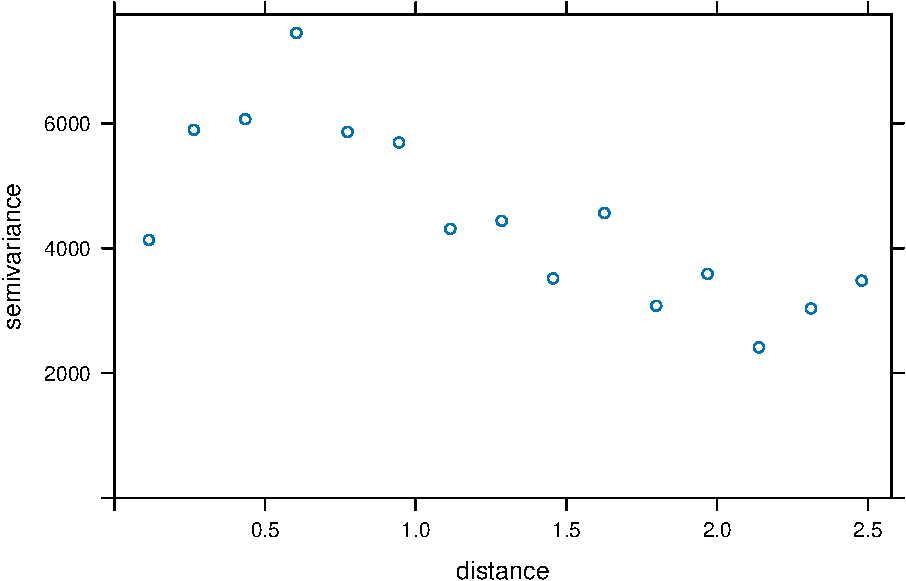
\includegraphics{_main_files/figure-latex/unnamed-chunk-35-3.pdf}

\begin{Shaded}
\begin{Highlighting}[]
\NormalTok{vg4 }\OtherTok{\textless{}{-}} \FunctionTok{variogram}\NormalTok{(}\FunctionTok{residuals.gam}\NormalTok{(m4, }\AttributeTok{type =} \StringTok{"response"}\NormalTok{) }\SpecialCharTok{\textasciitilde{}} \DecValTok{1}\NormalTok{, }\AttributeTok{loc =} \SpecialCharTok{\textasciitilde{}}\NormalTok{long }\SpecialCharTok{+}
\NormalTok{                  lat, }\AttributeTok{data =}\NormalTok{ train)}
\FunctionTok{plot}\NormalTok{(vg4)}
\end{Highlighting}
\end{Shaded}

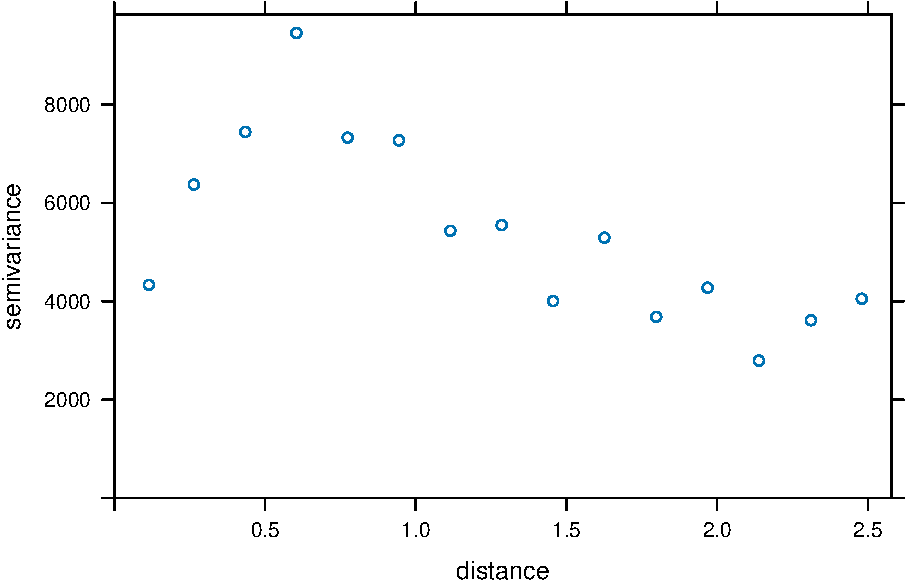
\includegraphics{_main_files/figure-latex/unnamed-chunk-35-4.pdf}

\hypertarget{model-checking-comparison}{%
\chapter{Model checking / comparison}\label{model-checking-comparison}}

\begin{Shaded}
\begin{Highlighting}[]
\NormalTok{E.y.m1 }\OtherTok{\textless{}{-}} \FunctionTok{predict}\NormalTok{(m1,}\AttributeTok{newdata=}\NormalTok{test,}\AttributeTok{type =} \StringTok{\textquotesingle{}response\textquotesingle{}}\NormalTok{)}
\FunctionTok{sum}\NormalTok{(}\FunctionTok{dnorm}\NormalTok{(test}\SpecialCharTok{$}\NormalTok{EGA,E.y.m1,}\AttributeTok{log=}\ConstantTok{TRUE}\NormalTok{))}
\end{Highlighting}
\end{Shaded}

\begin{verbatim}
## [1] -441616.1
\end{verbatim}

\begin{Shaded}
\begin{Highlighting}[]
\FunctionTok{mean}\NormalTok{((test}\SpecialCharTok{$}\NormalTok{EGA }\SpecialCharTok{{-}}\NormalTok{ E.y.m1)}\SpecialCharTok{\^{}}\DecValTok{2}\NormalTok{) }\CommentTok{\# Mean square error}
\end{Highlighting}
\end{Shaded}

\begin{verbatim}
## [1] 6540.623
\end{verbatim}

\begin{Shaded}
\begin{Highlighting}[]
\FunctionTok{mean}\NormalTok{(}\FunctionTok{abs}\NormalTok{(test}\SpecialCharTok{$}\NormalTok{EGA }\SpecialCharTok{{-}}\NormalTok{ E.y.m1)) }\CommentTok{\# Mean absolute error}
\end{Highlighting}
\end{Shaded}

\begin{verbatim}
## [1] 25.03223
\end{verbatim}

\begin{Shaded}
\begin{Highlighting}[]
\FunctionTok{plot}\NormalTok{(E.y.m1,test}\SpecialCharTok{$}\NormalTok{EGA,}\AttributeTok{xlab=}\StringTok{"Predicted expected value"}\NormalTok{,}\AttributeTok{ylab=}\StringTok{"New observed number of aphids"}\NormalTok{)}
\end{Highlighting}
\end{Shaded}

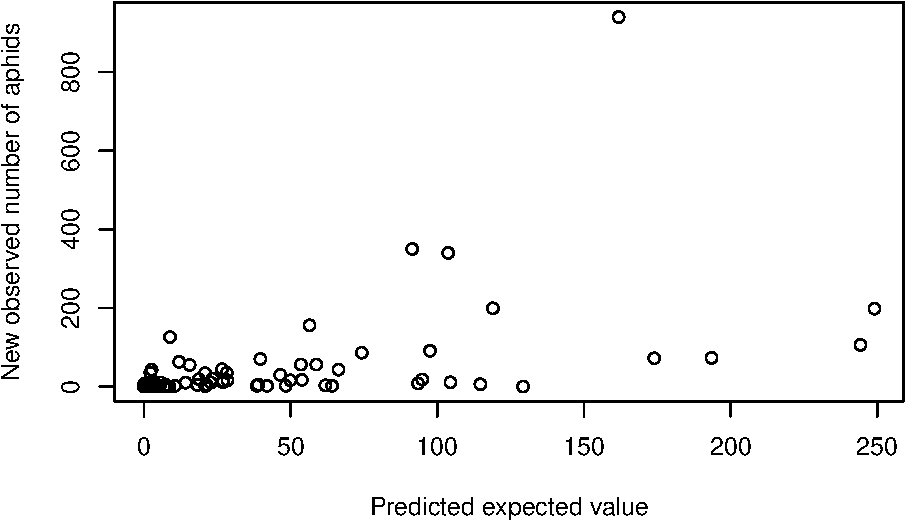
\includegraphics{_main_files/figure-latex/unnamed-chunk-36-1.pdf}

\begin{Shaded}
\begin{Highlighting}[]
\NormalTok{E.y.m2 }\OtherTok{\textless{}{-}} \FunctionTok{predict}\NormalTok{(m2,}\AttributeTok{newdata=}\NormalTok{test,}\AttributeTok{type =} \StringTok{\textquotesingle{}response\textquotesingle{}}\NormalTok{)}
\FunctionTok{sum}\NormalTok{(}\FunctionTok{dnorm}\NormalTok{(test}\SpecialCharTok{$}\NormalTok{EGA,E.y.m1,}\AttributeTok{log=}\ConstantTok{TRUE}\NormalTok{))}
\end{Highlighting}
\end{Shaded}

\begin{verbatim}
## [1] -441616.1
\end{verbatim}

\begin{Shaded}
\begin{Highlighting}[]
\FunctionTok{mean}\NormalTok{((test}\SpecialCharTok{$}\NormalTok{EGA }\SpecialCharTok{{-}}\NormalTok{ E.y.m2)}\SpecialCharTok{\^{}}\DecValTok{2}\NormalTok{) }\CommentTok{\# Mean square error}
\end{Highlighting}
\end{Shaded}

\begin{verbatim}
## [1] 7102.559
\end{verbatim}

\begin{Shaded}
\begin{Highlighting}[]
\FunctionTok{mean}\NormalTok{(}\FunctionTok{abs}\NormalTok{(test}\SpecialCharTok{$}\NormalTok{EGA }\SpecialCharTok{{-}}\NormalTok{ E.y.m2)) }\CommentTok{\# Mean absolute error}
\end{Highlighting}
\end{Shaded}

\begin{verbatim}
## [1] 25.41895
\end{verbatim}

\begin{Shaded}
\begin{Highlighting}[]
\FunctionTok{plot}\NormalTok{(E.y.m2,test}\SpecialCharTok{$}\NormalTok{EGA,}\AttributeTok{xlab=}\StringTok{"Predicted expected value"}\NormalTok{,}\AttributeTok{ylab=}\StringTok{"New observed number of aphids"}\NormalTok{)}
\end{Highlighting}
\end{Shaded}

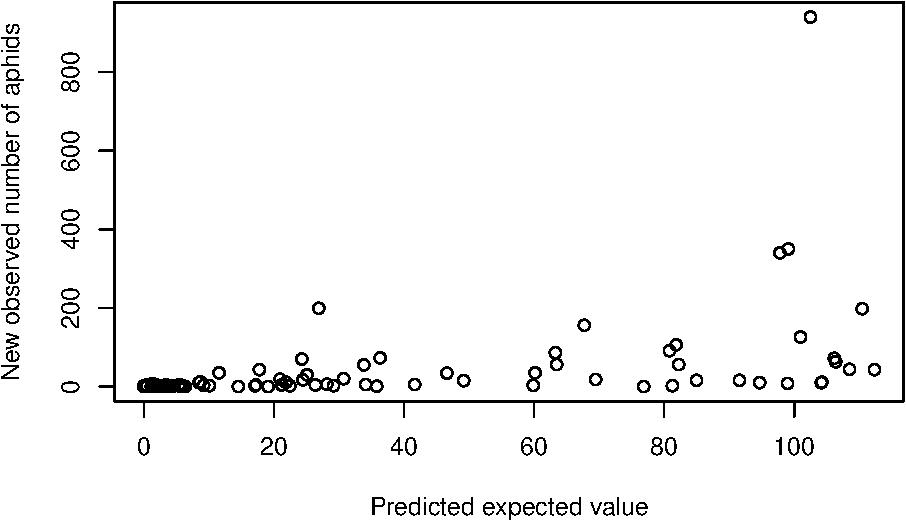
\includegraphics{_main_files/figure-latex/unnamed-chunk-36-2.pdf}

\begin{Shaded}
\begin{Highlighting}[]
\NormalTok{E.y.m3 }\OtherTok{\textless{}{-}} \FunctionTok{predict}\NormalTok{(m3,}\AttributeTok{newdata=}\NormalTok{test,}\AttributeTok{type =} \StringTok{\textquotesingle{}response\textquotesingle{}}\NormalTok{)}
\FunctionTok{sum}\NormalTok{(}\FunctionTok{dnorm}\NormalTok{(test}\SpecialCharTok{$}\NormalTok{EGA,E.y.m1,}\AttributeTok{log=}\ConstantTok{TRUE}\NormalTok{))}
\end{Highlighting}
\end{Shaded}

\begin{verbatim}
## [1] -441616.1
\end{verbatim}

\begin{Shaded}
\begin{Highlighting}[]
\FunctionTok{mean}\NormalTok{((test}\SpecialCharTok{$}\NormalTok{EGA }\SpecialCharTok{{-}}\NormalTok{ E.y.m3)}\SpecialCharTok{\^{}}\DecValTok{2}\NormalTok{) }\CommentTok{\# Mean square error}
\end{Highlighting}
\end{Shaded}

\begin{verbatim}
## [1] 7031.212
\end{verbatim}

\begin{Shaded}
\begin{Highlighting}[]
\FunctionTok{mean}\NormalTok{(}\FunctionTok{abs}\NormalTok{(test}\SpecialCharTok{$}\NormalTok{EGA }\SpecialCharTok{{-}}\NormalTok{ E.y.m3)) }\CommentTok{\# Mean absolute error}
\end{Highlighting}
\end{Shaded}

\begin{verbatim}
## [1] 22.5366
\end{verbatim}

\begin{Shaded}
\begin{Highlighting}[]
\FunctionTok{plot}\NormalTok{(E.y.m3,test}\SpecialCharTok{$}\NormalTok{EGA,}\AttributeTok{xlab=}\StringTok{"Predicted expected value"}\NormalTok{,}\AttributeTok{ylab=}\StringTok{"New observed number of aphids"}\NormalTok{)}
\end{Highlighting}
\end{Shaded}

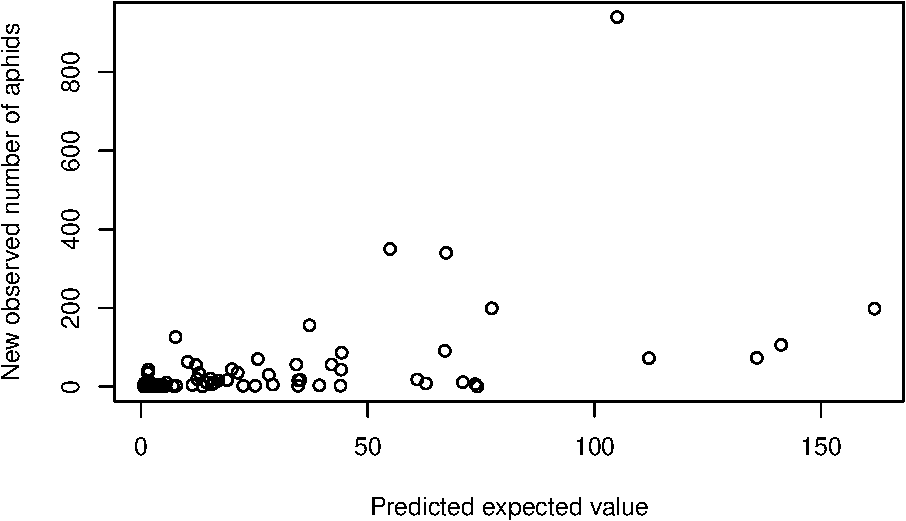
\includegraphics{_main_files/figure-latex/unnamed-chunk-36-3.pdf}

\begin{Shaded}
\begin{Highlighting}[]
\NormalTok{E.y.m4 }\OtherTok{\textless{}{-}} \FunctionTok{predict}\NormalTok{(m4,}\AttributeTok{newdata=}\NormalTok{test,}\AttributeTok{type =} \StringTok{\textquotesingle{}response\textquotesingle{}}\NormalTok{)}
\FunctionTok{sum}\NormalTok{(}\FunctionTok{dnorm}\NormalTok{(test}\SpecialCharTok{$}\NormalTok{EGA,E.y.m4,}\AttributeTok{log=}\ConstantTok{TRUE}\NormalTok{))}
\end{Highlighting}
\end{Shaded}

\begin{verbatim}
## [1] -513293.4
\end{verbatim}

\begin{Shaded}
\begin{Highlighting}[]
\FunctionTok{mean}\NormalTok{((test}\SpecialCharTok{$}\NormalTok{EGA }\SpecialCharTok{{-}}\NormalTok{ E.y.m4)}\SpecialCharTok{\^{}}\DecValTok{2}\NormalTok{) }\CommentTok{\# Mean square error}
\end{Highlighting}
\end{Shaded}

\begin{verbatim}
## [1] 7602.509
\end{verbatim}

\begin{Shaded}
\begin{Highlighting}[]
\FunctionTok{mean}\NormalTok{(}\FunctionTok{abs}\NormalTok{(test}\SpecialCharTok{$}\NormalTok{EGA }\SpecialCharTok{{-}}\NormalTok{ E.y.m4)) }\CommentTok{\# Mean absolute error}
\end{Highlighting}
\end{Shaded}

\begin{verbatim}
## [1] 34.07819
\end{verbatim}

\begin{Shaded}
\begin{Highlighting}[]
\FunctionTok{plot}\NormalTok{(E.y.m4,test}\SpecialCharTok{$}\NormalTok{EGA,}\AttributeTok{xlab=}\StringTok{"Predicted expected value"}\NormalTok{,}\AttributeTok{ylab=}\StringTok{"New observed number of aphids"}\NormalTok{)}
\end{Highlighting}
\end{Shaded}

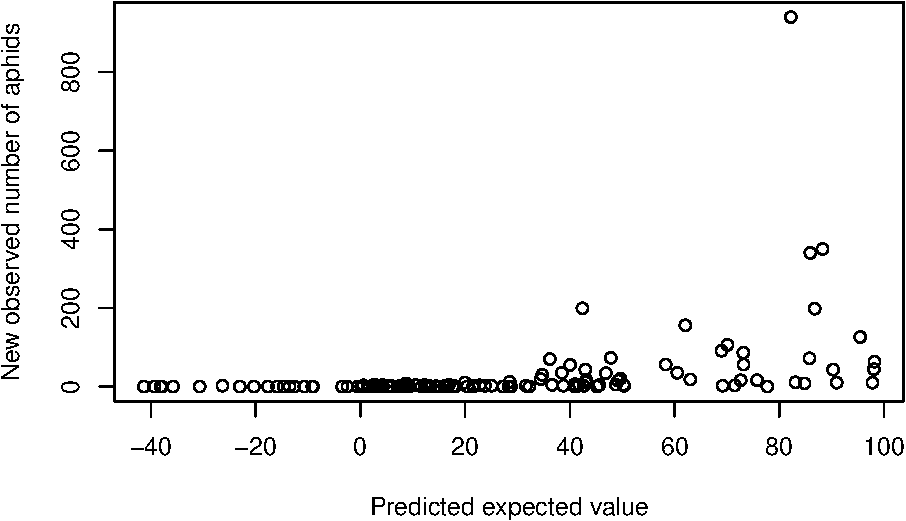
\includegraphics{_main_files/figure-latex/unnamed-chunk-36-4.pdf}

\hypertarget{predictions-in-space}{%
\section{Predictions in space}\label{predictions-in-space}}

\begin{Shaded}
\begin{Highlighting}[]
\NormalTok{newPoints }\OtherTok{\textless{}{-}} \FunctionTok{st\_sample}\NormalTok{(sf.kansas }\SpecialCharTok{\%\textgreater{}\%} \FunctionTok{st\_as\_sf}\NormalTok{(), }\AttributeTok{size =} \DecValTok{1000}\NormalTok{, }\AttributeTok{type =} \StringTok{"regular"}\NormalTok{) }\SpecialCharTok{\%\textgreater{}\%} 
  \FunctionTok{as}\NormalTok{(., }\StringTok{\textquotesingle{}Spatial\textquotesingle{}}\NormalTok{) }\SpecialCharTok{\%\textgreater{}\%} \FunctionTok{as.data.frame}\NormalTok{() }\SpecialCharTok{\%\textgreater{}\%} 
    \FunctionTok{rename}\NormalTok{(}\StringTok{"long"} \OtherTok{=} \StringTok{"coords.x1"}\NormalTok{, }
           \StringTok{"lat"} \OtherTok{=} \StringTok{"coords.x2"}\NormalTok{) }\SpecialCharTok{\%\textgreater{}\%} 
  \FunctionTok{cross\_join}\NormalTok{(}\FunctionTok{data.frame}\NormalTok{(}\AttributeTok{year =} \FunctionTok{as.factor}\NormalTok{(}\FunctionTok{c}\NormalTok{(}\StringTok{\textquotesingle{}2014\textquotesingle{}}\NormalTok{, }\StringTok{\textquotesingle{}2015\textquotesingle{}}\NormalTok{))))}

\NormalTok{pts.sample }\OtherTok{\textless{}{-}}\NormalTok{ newPoints}

\FunctionTok{coordinates}\NormalTok{(pts.sample) }\OtherTok{=}\ErrorTok{\textasciitilde{}}\NormalTok{ long }\SpecialCharTok{+}\NormalTok{ lat}
\FunctionTok{proj4string}\NormalTok{(pts.sample) }\OtherTok{\textless{}{-}} \FunctionTok{CRS}\NormalTok{(}\StringTok{"+proj=longlat +datum=WGS84 +no\_defs +ellps=WGS84 +towgs84=0,0,0"}\NormalTok{)}

\CommentTok{\# Calculate percentage of land area that is grassland withing 5 km of new points location}
\NormalTok{newPoints}\SpecialCharTok{$}\NormalTok{grass.perc }\OtherTok{\textless{}{-}} \FunctionTok{unlist}\NormalTok{(}\FunctionTok{lapply}\NormalTok{(raster}\SpecialCharTok{::}\FunctionTok{extract}\NormalTok{(rl.nlcd.grass,pts.sample,}\AttributeTok{buffer=}\DecValTok{5000}\NormalTok{),mean))}\SpecialCharTok{*}\DecValTok{100}

\CommentTok{\# Step 2: obtain predictions}
\NormalTok{newPoints}\SpecialCharTok{$}\NormalTok{pred.m1 }\OtherTok{\textless{}{-}} \FunctionTok{predict}\NormalTok{(m1, }\AttributeTok{newdata =}\NormalTok{ newPoints, }\AttributeTok{type =} \StringTok{"response"}\NormalTok{)}
\NormalTok{newPoints}\SpecialCharTok{$}\NormalTok{pred.m2 }\OtherTok{\textless{}{-}} \FunctionTok{predict}\NormalTok{(m2, }\AttributeTok{newdata =}\NormalTok{ newPoints, }\AttributeTok{type =} \StringTok{"response"}\NormalTok{)}
\NormalTok{newPoints}\SpecialCharTok{$}\NormalTok{pred.m3 }\OtherTok{\textless{}{-}} \FunctionTok{predict}\NormalTok{(m3, }\AttributeTok{newdata =}\NormalTok{ newPoints, }\AttributeTok{type =} \StringTok{"response"}\NormalTok{)}
\NormalTok{newPoints}\SpecialCharTok{$}\NormalTok{pred.m4 }\OtherTok{\textless{}{-}} \FunctionTok{predict}\NormalTok{(m4, }\AttributeTok{newdata =}\NormalTok{ newPoints, }\AttributeTok{type =} \StringTok{"response"}\NormalTok{)}
\end{Highlighting}
\end{Shaded}

\begin{Shaded}
\begin{Highlighting}[]
\CommentTok{\# Model 1}
\FunctionTok{ggplot}\NormalTok{() }\SpecialCharTok{+}
  \FunctionTok{geom\_tile}\NormalTok{(}\AttributeTok{data =}\NormalTok{ newPoints }\SpecialCharTok{\%\textgreater{}\%} \FunctionTok{filter}\NormalTok{(pred.m1 }\SpecialCharTok{\textless{}} \DecValTok{2000}\NormalTok{), }\FunctionTok{aes}\NormalTok{(}\AttributeTok{x =}\NormalTok{ long, }\AttributeTok{y =}\NormalTok{ lat, }\AttributeTok{fill =}\NormalTok{ pred.m1))}\SpecialCharTok{+}
  \FunctionTok{labs}\NormalTok{(}\AttributeTok{title =} \StringTok{"Model 1: Abundance of English grain aphids"}\NormalTok{, }\AttributeTok{x =} \StringTok{"Longitude"}\NormalTok{, }\AttributeTok{y =} \StringTok{"Latitude"}\NormalTok{)}\SpecialCharTok{+}
  \FunctionTok{scale\_fill\_viridis\_c}\NormalTok{(}\AttributeTok{option =} \StringTok{"D"}\NormalTok{, }\AttributeTok{alpha =} \FloatTok{0.95}\NormalTok{)}\SpecialCharTok{+}
  \FunctionTok{theme}\NormalTok{(}\AttributeTok{legend.background =} \FunctionTok{element\_rect}\NormalTok{(}\AttributeTok{fill =} \StringTok{"transparent"}\NormalTok{, }\AttributeTok{colour =} \ConstantTok{NA}\NormalTok{),}
        \AttributeTok{panel.grid =} \FunctionTok{element\_blank}\NormalTok{(),}
        \AttributeTok{plot.margin =} \FunctionTok{unit}\NormalTok{(}\FunctionTok{c}\NormalTok{(}\FloatTok{0.5}\NormalTok{, }\FloatTok{0.5}\NormalTok{, }\FloatTok{0.5}\NormalTok{, }\FloatTok{0.5}\NormalTok{), }\StringTok{"lines"}\NormalTok{),}
        \AttributeTok{panel.background =} \FunctionTok{element\_rect}\NormalTok{(}\AttributeTok{fill =} \StringTok{"grey90"}\NormalTok{),}
        \AttributeTok{axis.text =} \FunctionTok{element\_text}\NormalTok{(}\AttributeTok{size =} \DecValTok{12}\NormalTok{), }
        \AttributeTok{axis.text.x =} \FunctionTok{element\_text}\NormalTok{(}\AttributeTok{angle =} \DecValTok{90}\NormalTok{, }\AttributeTok{vjust =} \FloatTok{0.5}\NormalTok{, }\AttributeTok{hjust =} \DecValTok{1}\NormalTok{),}
        \AttributeTok{strip.text =} \FunctionTok{element\_text}\NormalTok{(}\AttributeTok{size =} \DecValTok{11}\NormalTok{, }\AttributeTok{face =} \StringTok{"bold"}\NormalTok{),}
        \AttributeTok{title =} \FunctionTok{element\_text}\NormalTok{(}\AttributeTok{size =} \DecValTok{12}\NormalTok{, }\AttributeTok{face =} \StringTok{"bold"}\NormalTok{),}
        \AttributeTok{axis.title =} \FunctionTok{element\_text}\NormalTok{(}\AttributeTok{size =} \DecValTok{14}\NormalTok{))}\SpecialCharTok{+}
  \FunctionTok{facet\_wrap}\NormalTok{(}\SpecialCharTok{\textasciitilde{}}\NormalTok{year) }\SpecialCharTok{+}
  \FunctionTok{geom\_point}\NormalTok{(}\AttributeTok{data =}\NormalTok{ df1, }\FunctionTok{aes}\NormalTok{(}\AttributeTok{x =}\NormalTok{ long, }\AttributeTok{y =}\NormalTok{ lat, }\AttributeTok{size =}\NormalTok{ EGA), }\AttributeTok{color =} \StringTok{"white"}\NormalTok{, }\AttributeTok{shape =} \DecValTok{21}\NormalTok{) }
\end{Highlighting}
\end{Shaded}

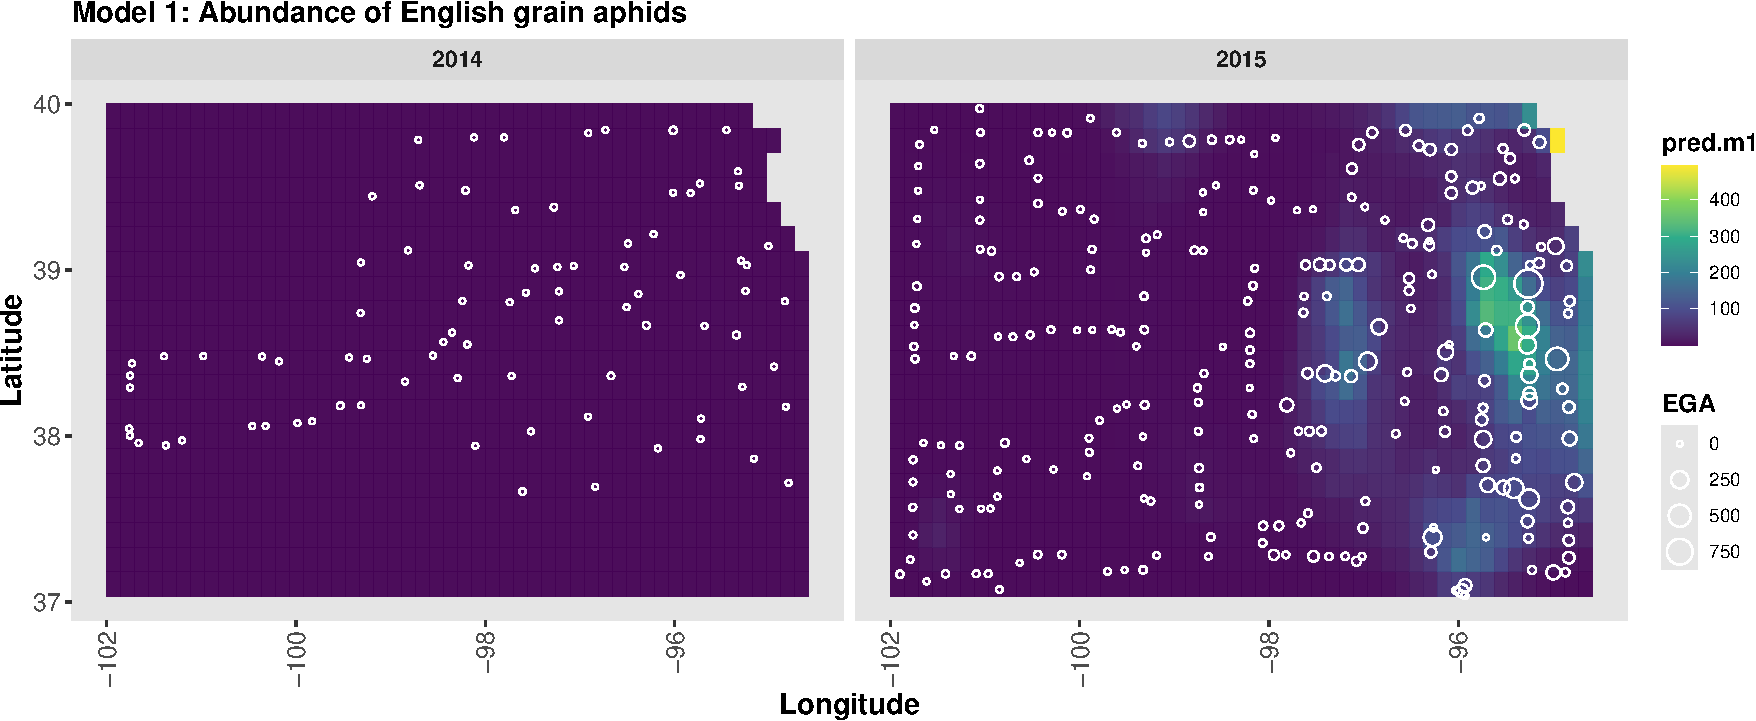
\includegraphics{_main_files/figure-latex/unnamed-chunk-38-1.pdf}

\begin{Shaded}
\begin{Highlighting}[]
\CommentTok{\# Model 2}
\FunctionTok{ggplot}\NormalTok{() }\SpecialCharTok{+}
  \FunctionTok{geom\_tile}\NormalTok{(}\AttributeTok{data =}\NormalTok{ newPoints, }\FunctionTok{aes}\NormalTok{(}\AttributeTok{x =}\NormalTok{ long, }\AttributeTok{y =}\NormalTok{ lat, }\AttributeTok{fill =}\NormalTok{ pred.m2))}\SpecialCharTok{+}
  \FunctionTok{labs}\NormalTok{(}\AttributeTok{title =} \StringTok{"Model 2: Abundance of English grain aphids"}\NormalTok{, }\AttributeTok{x =} \StringTok{"Longitude"}\NormalTok{, }\AttributeTok{y =} \StringTok{"Latitude"}\NormalTok{)}\SpecialCharTok{+}
  \FunctionTok{scale\_fill\_viridis\_c}\NormalTok{(}\AttributeTok{option =} \StringTok{"D"}\NormalTok{, }\AttributeTok{alpha =} \FloatTok{0.95}\NormalTok{)}\SpecialCharTok{+}
  \FunctionTok{theme}\NormalTok{(}\AttributeTok{legend.background =} \FunctionTok{element\_rect}\NormalTok{(}\AttributeTok{fill =} \StringTok{"transparent"}\NormalTok{, }\AttributeTok{colour =} \ConstantTok{NA}\NormalTok{),}
        \AttributeTok{panel.grid =} \FunctionTok{element\_blank}\NormalTok{(),}
        \AttributeTok{plot.margin =} \FunctionTok{unit}\NormalTok{(}\FunctionTok{c}\NormalTok{(}\FloatTok{0.5}\NormalTok{, }\FloatTok{0.5}\NormalTok{, }\FloatTok{0.5}\NormalTok{, }\FloatTok{0.5}\NormalTok{), }\StringTok{"lines"}\NormalTok{),}
        \AttributeTok{panel.background =} \FunctionTok{element\_rect}\NormalTok{(}\AttributeTok{fill =} \StringTok{"grey90"}\NormalTok{),}
        \AttributeTok{axis.text =} \FunctionTok{element\_text}\NormalTok{(}\AttributeTok{size =} \DecValTok{12}\NormalTok{), }
        \AttributeTok{axis.text.x =} \FunctionTok{element\_text}\NormalTok{(}\AttributeTok{angle =} \DecValTok{90}\NormalTok{, }\AttributeTok{vjust =} \FloatTok{0.5}\NormalTok{, }\AttributeTok{hjust =} \DecValTok{1}\NormalTok{),}
        \AttributeTok{strip.text =} \FunctionTok{element\_text}\NormalTok{(}\AttributeTok{size =} \DecValTok{11}\NormalTok{, }\AttributeTok{face =} \StringTok{"bold"}\NormalTok{),}
        \AttributeTok{title =} \FunctionTok{element\_text}\NormalTok{(}\AttributeTok{size =} \DecValTok{12}\NormalTok{, }\AttributeTok{face =} \StringTok{"bold"}\NormalTok{),}
        \AttributeTok{axis.title =} \FunctionTok{element\_text}\NormalTok{(}\AttributeTok{size =} \DecValTok{14}\NormalTok{))}\SpecialCharTok{+}
  \FunctionTok{facet\_wrap}\NormalTok{(}\SpecialCharTok{\textasciitilde{}}\NormalTok{year) }\SpecialCharTok{+}
  \FunctionTok{geom\_point}\NormalTok{(}\AttributeTok{data =}\NormalTok{ df1, }\FunctionTok{aes}\NormalTok{(}\AttributeTok{x =}\NormalTok{ long, }\AttributeTok{y =}\NormalTok{ lat, }\AttributeTok{size =}\NormalTok{ EGA), }\AttributeTok{color =} \StringTok{"white"}\NormalTok{, }\AttributeTok{shape =} \DecValTok{21}\NormalTok{) }
\end{Highlighting}
\end{Shaded}

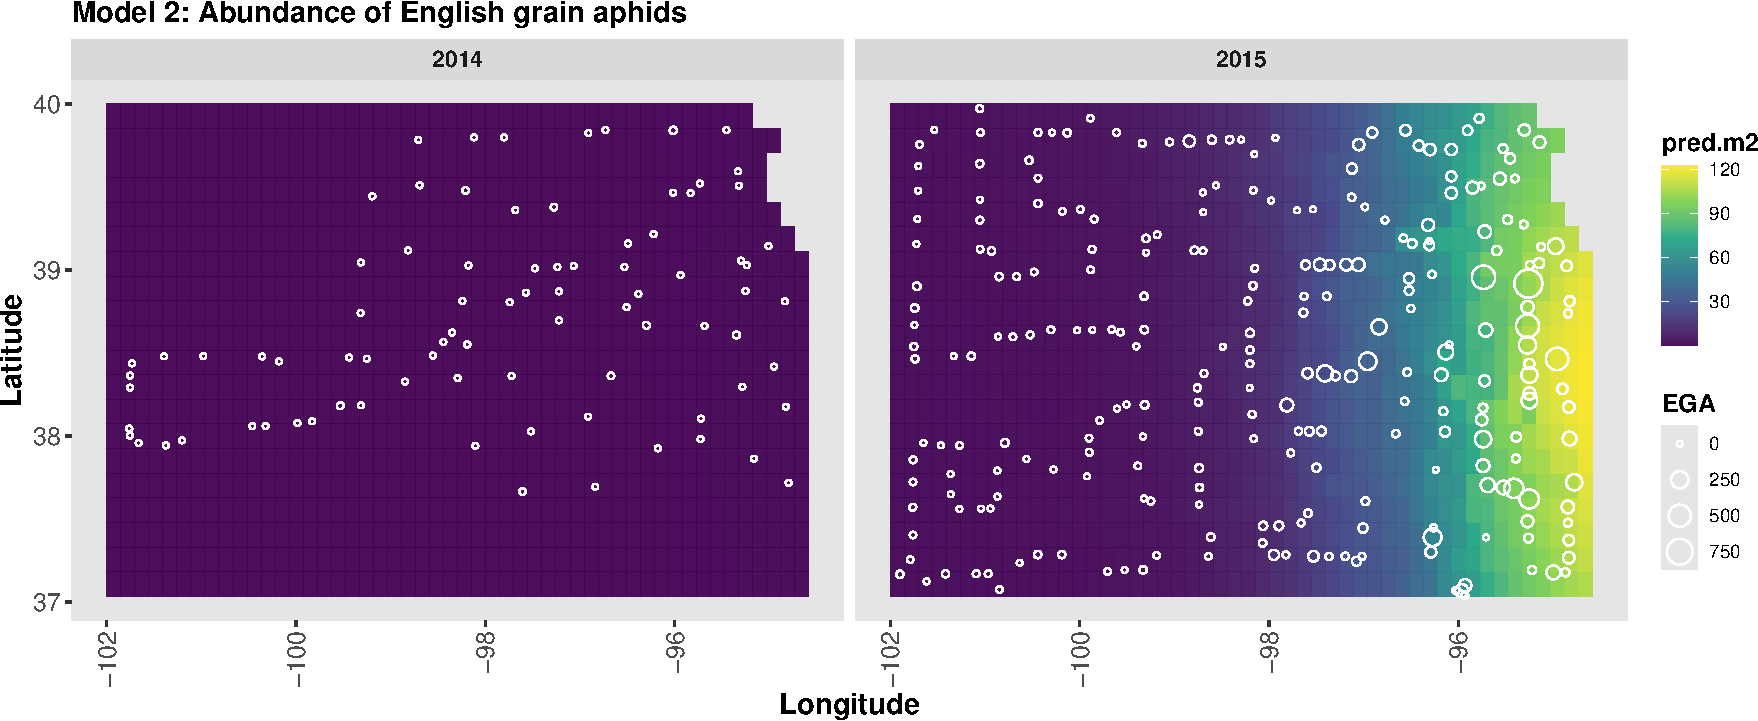
\includegraphics{_main_files/figure-latex/unnamed-chunk-39-1.pdf}

\begin{Shaded}
\begin{Highlighting}[]
\CommentTok{\# Model 3}
\FunctionTok{ggplot}\NormalTok{() }\SpecialCharTok{+}
  \FunctionTok{geom\_tile}\NormalTok{(}\AttributeTok{data =}\NormalTok{ newPoints }\SpecialCharTok{\%\textgreater{}\%} \FunctionTok{filter}\NormalTok{(pred.m3 }\SpecialCharTok{\textless{}} \DecValTok{1000}\NormalTok{), }\FunctionTok{aes}\NormalTok{(}\AttributeTok{x =}\NormalTok{ long, }\AttributeTok{y =}\NormalTok{ lat, }\AttributeTok{fill =}\NormalTok{ pred.m3))}\SpecialCharTok{+}
  \FunctionTok{labs}\NormalTok{(}\AttributeTok{title =} \StringTok{"Model 3: Abundance of English grain aphids"}\NormalTok{, }\AttributeTok{x =} \StringTok{"Longitude"}\NormalTok{, }\AttributeTok{y =} \StringTok{"Latitude"}\NormalTok{)}\SpecialCharTok{+}
  \FunctionTok{scale\_fill\_viridis\_c}\NormalTok{(}\AttributeTok{option =} \StringTok{"D"}\NormalTok{, }\AttributeTok{alpha =} \FloatTok{0.95}\NormalTok{)}\SpecialCharTok{+}
  \FunctionTok{theme}\NormalTok{(}\AttributeTok{legend.background =} \FunctionTok{element\_rect}\NormalTok{(}\AttributeTok{fill =} \StringTok{"transparent"}\NormalTok{, }\AttributeTok{colour =} \ConstantTok{NA}\NormalTok{),}
        \AttributeTok{panel.grid =} \FunctionTok{element\_blank}\NormalTok{(),}
        \AttributeTok{plot.margin =} \FunctionTok{unit}\NormalTok{(}\FunctionTok{c}\NormalTok{(}\FloatTok{0.5}\NormalTok{, }\FloatTok{0.5}\NormalTok{, }\FloatTok{0.5}\NormalTok{, }\FloatTok{0.5}\NormalTok{), }\StringTok{"lines"}\NormalTok{),}
        \AttributeTok{panel.background =} \FunctionTok{element\_rect}\NormalTok{(}\AttributeTok{fill =} \StringTok{"grey90"}\NormalTok{),}
        \AttributeTok{axis.text =} \FunctionTok{element\_text}\NormalTok{(}\AttributeTok{size =} \DecValTok{12}\NormalTok{), }
        \AttributeTok{axis.text.x =} \FunctionTok{element\_text}\NormalTok{(}\AttributeTok{angle =} \DecValTok{90}\NormalTok{, }\AttributeTok{vjust =} \FloatTok{0.5}\NormalTok{, }\AttributeTok{hjust =} \DecValTok{1}\NormalTok{),}
        \AttributeTok{strip.text =} \FunctionTok{element\_text}\NormalTok{(}\AttributeTok{size =} \DecValTok{11}\NormalTok{, }\AttributeTok{face =} \StringTok{"bold"}\NormalTok{),}
        \AttributeTok{title =} \FunctionTok{element\_text}\NormalTok{(}\AttributeTok{size =} \DecValTok{12}\NormalTok{, }\AttributeTok{face =} \StringTok{"bold"}\NormalTok{),}
        \AttributeTok{axis.title =} \FunctionTok{element\_text}\NormalTok{(}\AttributeTok{size =} \DecValTok{14}\NormalTok{))}\SpecialCharTok{+}
  \FunctionTok{facet\_wrap}\NormalTok{(}\SpecialCharTok{\textasciitilde{}}\NormalTok{year) }\SpecialCharTok{+}
  \FunctionTok{geom\_point}\NormalTok{(}\AttributeTok{data =}\NormalTok{ df1, }\FunctionTok{aes}\NormalTok{(}\AttributeTok{x =}\NormalTok{ long, }\AttributeTok{y =}\NormalTok{ lat, }\AttributeTok{size =}\NormalTok{ EGA), }\AttributeTok{color =} \StringTok{"white"}\NormalTok{, }\AttributeTok{shape =} \DecValTok{21}\NormalTok{) }
\end{Highlighting}
\end{Shaded}

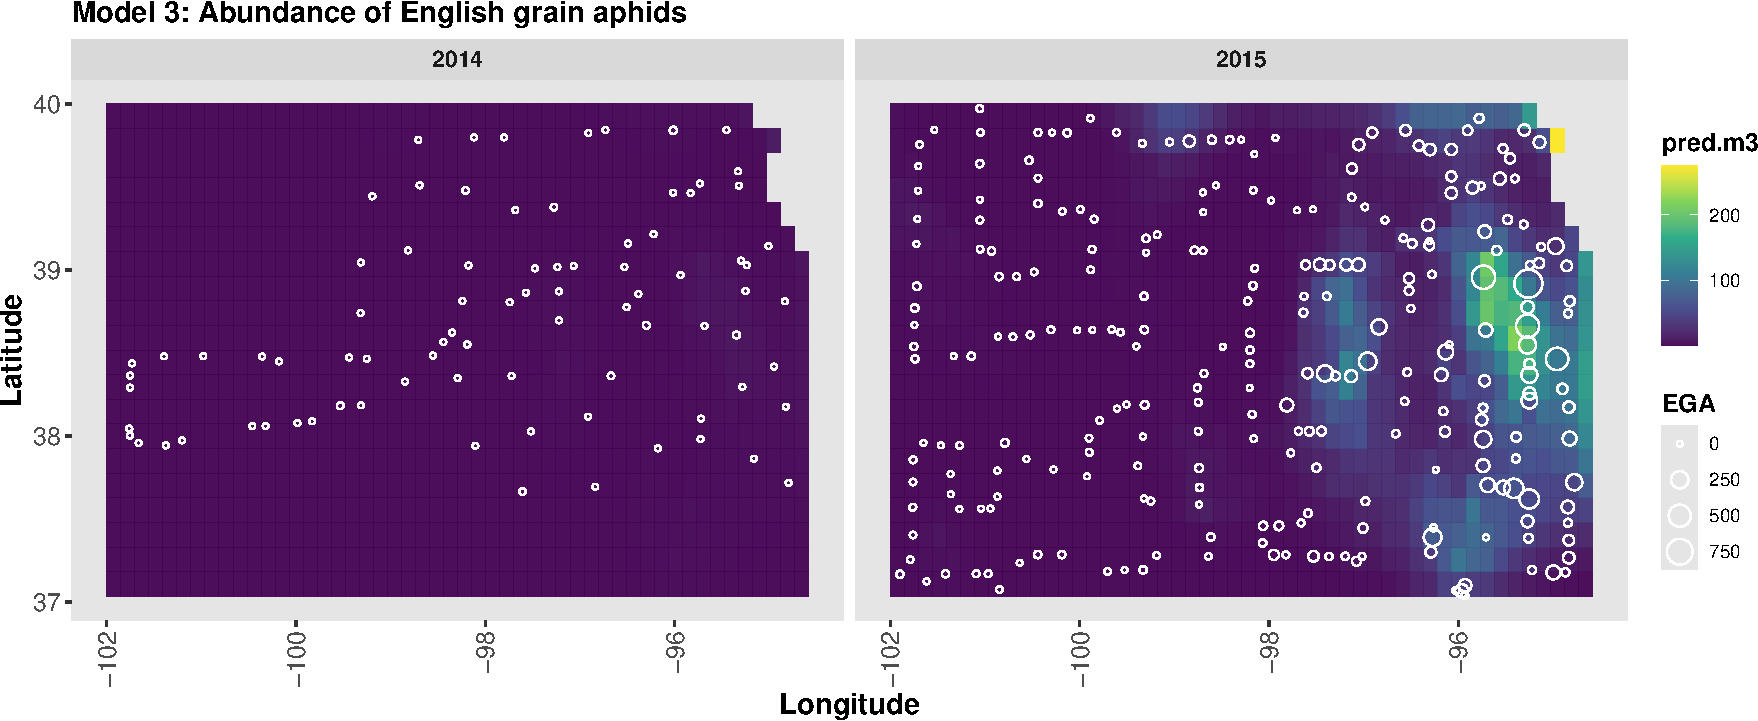
\includegraphics{_main_files/figure-latex/unnamed-chunk-40-1.pdf}

\begin{Shaded}
\begin{Highlighting}[]
\CommentTok{\# Model 4}
\FunctionTok{ggplot}\NormalTok{() }\SpecialCharTok{+}
  \FunctionTok{geom\_tile}\NormalTok{(}\AttributeTok{data =}\NormalTok{ newPoints, }\FunctionTok{aes}\NormalTok{(}\AttributeTok{x =}\NormalTok{ long, }\AttributeTok{y =}\NormalTok{ lat, }\AttributeTok{fill =}\NormalTok{ pred.m4))}\SpecialCharTok{+}
  \FunctionTok{labs}\NormalTok{(}\AttributeTok{title =} \StringTok{"Model 4: Abundance of English grain aphids"}\NormalTok{, }\AttributeTok{x =} \StringTok{"Longitude"}\NormalTok{, }\AttributeTok{y =} \StringTok{"Latitude"}\NormalTok{)}\SpecialCharTok{+}
  \FunctionTok{scale\_fill\_viridis\_c}\NormalTok{(}\AttributeTok{option =} \StringTok{"D"}\NormalTok{, }\AttributeTok{alpha =} \FloatTok{0.95}\NormalTok{)}\SpecialCharTok{+}
  \FunctionTok{theme}\NormalTok{(}\AttributeTok{legend.background =} \FunctionTok{element\_rect}\NormalTok{(}\AttributeTok{fill =} \StringTok{"transparent"}\NormalTok{, }\AttributeTok{colour =} \ConstantTok{NA}\NormalTok{),}
        \AttributeTok{panel.grid =} \FunctionTok{element\_blank}\NormalTok{(),}
        \AttributeTok{plot.margin =} \FunctionTok{unit}\NormalTok{(}\FunctionTok{c}\NormalTok{(}\FloatTok{0.5}\NormalTok{, }\FloatTok{0.5}\NormalTok{, }\FloatTok{0.5}\NormalTok{, }\FloatTok{0.5}\NormalTok{), }\StringTok{"lines"}\NormalTok{),}
        \AttributeTok{panel.background =} \FunctionTok{element\_rect}\NormalTok{(}\AttributeTok{fill =} \StringTok{"grey90"}\NormalTok{),}
        \AttributeTok{axis.text =} \FunctionTok{element\_text}\NormalTok{(}\AttributeTok{size =} \DecValTok{12}\NormalTok{), }
        \AttributeTok{axis.text.x =} \FunctionTok{element\_text}\NormalTok{(}\AttributeTok{angle =} \DecValTok{90}\NormalTok{, }\AttributeTok{vjust =} \FloatTok{0.5}\NormalTok{, }\AttributeTok{hjust =} \DecValTok{1}\NormalTok{),}
        \AttributeTok{strip.text =} \FunctionTok{element\_text}\NormalTok{(}\AttributeTok{size =} \DecValTok{11}\NormalTok{, }\AttributeTok{face =} \StringTok{"bold"}\NormalTok{),}
        \AttributeTok{title =} \FunctionTok{element\_text}\NormalTok{(}\AttributeTok{size =} \DecValTok{12}\NormalTok{, }\AttributeTok{face =} \StringTok{"bold"}\NormalTok{),}
        \AttributeTok{axis.title =} \FunctionTok{element\_text}\NormalTok{(}\AttributeTok{size =} \DecValTok{14}\NormalTok{))}\SpecialCharTok{+}
  \FunctionTok{facet\_wrap}\NormalTok{(}\SpecialCharTok{\textasciitilde{}}\NormalTok{year) }\SpecialCharTok{+}
  \FunctionTok{geom\_point}\NormalTok{(}\AttributeTok{data =}\NormalTok{ df1, }\FunctionTok{aes}\NormalTok{(}\AttributeTok{x =}\NormalTok{ long, }\AttributeTok{y =}\NormalTok{ lat, }\AttributeTok{size =}\NormalTok{ EGA), }\AttributeTok{color =} \StringTok{"white"}\NormalTok{, }\AttributeTok{shape =} \DecValTok{21}\NormalTok{) }
\end{Highlighting}
\end{Shaded}

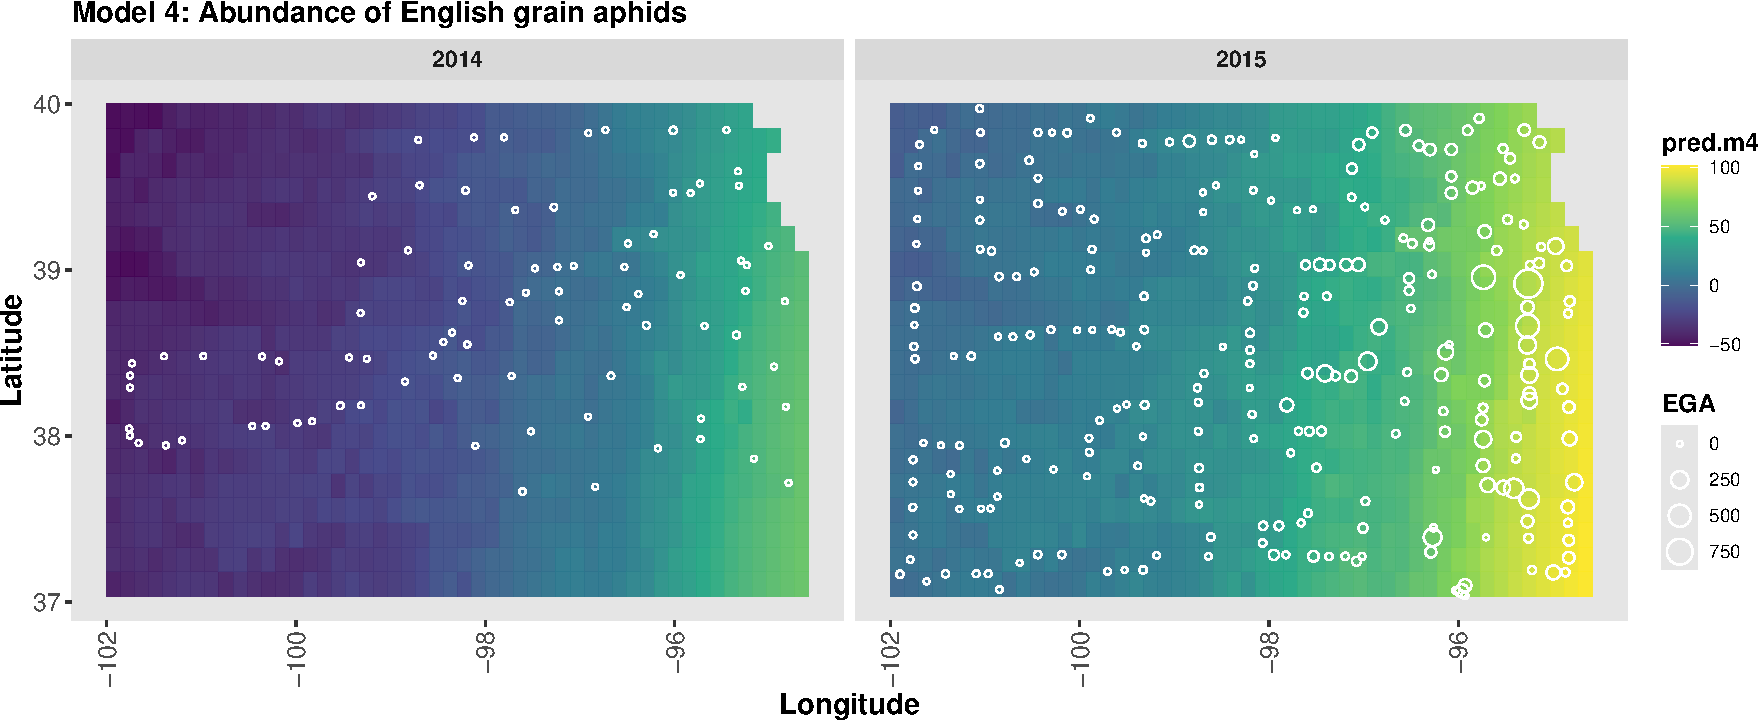
\includegraphics{_main_files/figure-latex/unnamed-chunk-41-1.pdf}

\hypertarget{summary}{%
\subsection{Summary}\label{summary}}

The model with the most accurate prediction is the negative binomial in the 1st place (MAE = 23 English Grain Aphid), and the gaussian in the 2nd place(MAE = 37 English Grain Aphid). In real world terms, however, the gaussian distribution assumes continuous observations in all the range of numbers (\(\overset{+}{\_} \infty\)) which does not correlate with count data (positive integers). In addition, when we predict the number of aphids for Kansas, the poisson and the zero inflated poisson estimate extreme high values in the north west region.

  \bibliography{book.bib,packages.bib}

\end{document}
